%% Run LaTeX on this file several times to get Table of Contents,
%% cross-references, and citations.

\documentclass[11pt]{book}
\usepackage{gvv}
\usepackage{gvv-book-bkup}
%\usepackage{Wiley-AuthoringTemplate}
\usepackage[sectionbib,authoryear]{natbib}% for name-date citation comment the below line
%\usepackage[sectionbib,numbers]{natbib}% for numbered citation comment the above line

%%********************************************************************%%
%%       How many levels of section head would you like numbered?     %%
%% 0= no section numbers, 1= section, 2= subsection, 3= subsubsection %%
\setcounter{secnumdepth}{3}
%%********************************************************************%%
%%**********************************************************************%%
%%     How many levels of section head would you like to appear in the  %%
%%				Table of Contents?			%%
%% 0= chapter, 1= section, 2= subsection, 3= subsubsection titles.	%%
\setcounter{tocdepth}{2}
%%**********************************************************************%%

%\includeonly{ch01}
\makeindex

\begin{document}

\frontmatter
%%%%%%%%%%%%%%%%%%%%%%%%%%%%%%%%%%%%%%%%%%%%%%%%%%%%%%%%%%%%%%%%
%% Title Pages
%% Wiley will provide title and copyright page, but you can make
%% your own titlepages if you'd like anyway
%% Setting up title pages, type in the appropriate names here:

\booktitle{Matrix Analysis}

\subtitle{Through JEE}

\AuAff{G. V. V. Sharma}


%% \\ will start a new line.
%% You may add \affil{} for affiliation, ie,
%\authors{Robert M. Groves\\
%\affil{Universitat de les Illes Balears}
%Floyd J. Fowler, Jr.\\
%\affil{University of New Mexico}
%}

%% Print Half Title and Title Page:
%\halftitlepage
\titlepage

%%%%%%%%%%%%%%%%%%%%%%%%%%%%%%%%%%%%%%%%%%%%%%%%%%%%%%%%%%%%%%%%
%% Copyright Page

\begin{copyrightpage}{2022}
%Title, etc
\end{copyrightpage}

% Note, you must use \ to start indented lines, ie,
% 
% \begin{copyrightpage}{2004}
% Survey Methodology / Robert M. Groves . . . [et al.].
% \       p. cm.---(Wiley series in survey methodology)
% \    ``Wiley-Interscience."
% \    Includes bibliographical references and index.
% \    ISBN 0-471-48348-6 (pbk.)
% \    1. Surveys---Methodology.  2. Social 
% \  sciences---Research---Statistical methods.  I. Groves, Robert M.  II. %
% Series.\\

% HA31.2.S873 2004
% 001.4'33---dc22                                             2004044064
% \end{copyrightpage}

%%%%%%%%%%%%%%%%%%%%%%%%%%%%%%%%%%%%%%%%%%%%%%%%%%%%%%%%%%%%%%%%
%% Only Dedication (optional) 

%\dedication{To my parents}

\tableofcontents

%\listoffigures %optional
%\listoftables  %optional

%% or Contributor Page for edited books
%% before \tableofcontents

%%%%%%%%%%%%%%%%%%%%%%%%%%%%%%%%%%%%%%%%%%%%%%%%%%%%%%%%%%%%%%%%
%  Contributors Page for Edited Book
%%%%%%%%%%%%%%%%%%%%%%%%%%%%%%%%%%%%%%%%%%%%%%%%%%%%%%%%%%%%%%%%

% If your book has chapters written by different authors,
% you'll need a Contributors page.

% Use \begin{contributors}...\end{contributors} and
% then enter each author with the \name{} command, followed
% by the affiliation information.

% \begin{contributors}
% \name{Masayki Abe,} Fujitsu Laboratories Ltd., Fujitsu Limited, Atsugi, Japan
%
% \name{L. A. Akers,} Center for Solid State Electronics Research, Arizona State University, Tempe, Arizona
%
% \name{G. H. Bernstein,} Department of Electrical and Computer Engineering, University of Notre Dame, Notre Dame, South Bend, Indiana; formerly of
% Center for Solid State Electronics Research, Arizona
% State University, Tempe, Arizona 
% \end{contributors}

%%%%%%%%%%%%%%%%%%%%%%%%%%%%%%%%%%%%%%%%%%%%%%%%%%%%%%%%%%%%%%%%
% Optional Foreword:

%\begin{foreword}
%\lipsum[1-2]
%\end{foreword}

%%%%%%%%%%%%%%%%%%%%%%%%%%%%%%%%%%%%%%%%%%%%%%%%%%%%%%%%%%%%%%%%
% Optional Preface:

%\begin{preface}
%\lipsum[1-1]
%\prefaceauthor{}
%\where{place\\
% date}
%\end{preface}

% ie,
% \begin{preface}
% This is an example preface.
% \prefaceauthor{R. K. Watts}
% \where{Durham, North Carolina\\
% September, 2004}

%%%%%%%%%%%%%%%%%%%%%%%%%%%%%%%%%%%%%%%%%%%%%%%%%%%%%%%%%%%%%%%%
% Optional Acknowledgments:

%\acknowledgments
%\lipsum[1-2]
%\authorinitials{I. R. S.}  

%%%%%%%%%%%%%%%%%%%%%%%%%%%%%%%%
%% Glossary Type of Environment:

% \begin{glossary}
% \term{<term>}{<description>}
% \end{glossary}

%%%%%%%%%%%%%%%%%%%%%%%%%%%%%%%%
%\begin{acronyms}
%\acro{ASTA}{Arrivals See Time Averages}
%\acro{BHCA}{Busy Hour Call Attempts}
%\acro{BR}{Bandwidth Reservation}
%\acro{b.u.}{bandwidth unit(s)}
%\acro{CAC}{Call / Connection Admission Control}
%\acro{CBP}{Call Blocking Probability(-ies)}
%\acro{CCS}{Centum Call Seconds}
%\acro{CDTM}{Connection Dependent Threshold Model}
%\acro{CS}{Complete Sharing}
%\acro{DiffServ}{Differentiated Services}
%\acro{EMLM}{Erlang Multirate Loss Model}
%\acro{erl}{The Erlang unit of traffic-load}
%\acro{FIFO}{First in - First out}
%\acro{GB}{Global balance}
%\acro{GoS}{Grade of Service}
%\acro{ICT}{Information and Communication Technology}
%\acro{IntServ}{Integrated Services}
%\acro{IP}{Internet Protocol}
%\acro{ITU-T}{International Telecommunication Unit -- Standardization sector}
%\acro{LB}{Local balance}
%\acro{LHS}{Left hand side}
%\acro{LIFO}{Last in - First out}
%\acro{MMPP}{Markov Modulated Poisson Process}
%\acro{MPLS}{Multiple Protocol Labeling Switching}
%\acro{MRM}{Multi-Retry Model}
%\acro{MTM}{Multi-Threshold Model}
%\acro{PASTA}{Poisson Arrivals See Time Averages}
%\acro{PDF}{Probability Distribution Function}
%\acro{pdf}{probability density function}
%\acro{PFS}{Product Form Solution}
%\acro{QoS}{Quality of Service}
%\acro{r.v.}{random variable(s)}
%\acro{RED}{random early detection}
%\acro{RHS}{Right hand side}
%\acro{RLA}{Reduced Load Approximation}
%\acro{SIRO}{service in random order}
%\acro{SRM}{Single-Retry Model}
%\acro{STM}{Single-Threshold Model}
%\acro{TCP}{Transport Control Protocol}
%\acro{TH}{Threshold(s)}
%\acro{UDP}{User Datagram Protocol}
%\end{acronyms}

\setcounter{page}{1}

\begin{introduction}
This book links high school coordinate geometry to linear algebra and matrix analysis through solved problems.

\end{introduction}

\mainmatter

\chapter{Straight Line and Pair of Straight Lines}
\documentclass[12pt]{article}
\usepackage{graphicx}
\usepackage{enumerate}
\usepackage{amsmath}
\usepackage{ragged2e}
\newcommand{\myvec}[1]{\ensuremath{\begin{pmatrix}#1\end{pmatrix}}}
\newcommand{\mydet}[1]{\ensuremath{\begin{vmatrix}#1\end{vmatrix}}}
\providecommand{\brak}[1]{\ensuremath{\left(#1\right)}}
\providecommand{\lbrak}[1]{\ensuremath{\left(#1\right.}}
\providecommand{\rbrak}[1]{\ensuremath{\left(#1\right)}}
\providecommand{\sbrak}[1]{\ensuremath{{}\left[#1\right]}}
\let\vec\mathbf

\begin{document}
\begin{center}
\textbf\large{CHAPTER-7 \\ Straight Line and Pair of Straight Lines}

\end{center}


\section*{Section-A    [JEE Advanced/IIT-JEE]}
\section*{A    :  Fill in the Blanks}
\begin{enumerate}

\item  The area enclosed with in the curves $|x|+|y|$ is.........  (1981) \\
\item  $y=10^x$ is the reflection of $y=\log_10^x $ in the line whose equation is.........(1982)\\
\item The set of lines $ax+by+c=0$ where $3a+2b+4c=0$ is concurrent at the point..........(1982)\\
\item  Given the points $\vec{A}(0,4)$ and $\vec{B}(0,-4)$, the equation of the locus of the point P(x,y) such that$|\vec{AP}-\vec{BP}|=6$ is.............(1983)\\
\item  If $a,b and c$ are in A.P.. then the straight line $ax+by+c=0$ will always pass through a fixed point whose coordinates are........(1984)\\
\item  The orthocenter of the triangle formed by the lines $x+y=1, 2x+3y=6  and  4x-y+4=0$ lies in quadrant number............(1985)\\
\item Let the algebraic sum of the perpendicular distances from the points (2,0), (0,2) and (1,1)to a variable straight line be zero; then the line passes through a fixed point whose cordinates are.........(1991)\\
\item The vertices of a triangle are $\vec{A}(-1,-7)$, $\vec{B}(5,1)$and $\vec{C}(1,4)$. The equation of the bisector of the angle $\angle{ABC}$ is........(1993)

\end{enumerate}

\section*{B    :    True/False}

\begin{enumerate}


\item  The sraight line $5x+4y=0$ passes through the point of intersection of the straight lines $x+2y-10=0$ and $2x+5+6=0$.(1983)\\
\item The lines $2x+3y=19=0$ $9x+6y-17=0$ cut the coordinate axes in concyclic points.(1988)\\
\end{enumerate}

\section*{C  :   MCQ'S with One Correct Answer}

\begin{enumerate}
\item The points$(a,b),(0,0)(a,b)$ and $(a^2,ab)$ are: (1979)
\begin{enumerate}
\item Collinear
\item Vertices of a parallelogram
\item Vertices of a rectangle
\item None of the above
\end{enumerate}
\item The point $(4,1)$ undergose the following three transformations successively.
\begin{enumerate}[i]
\item Reflection about the line y=x\\
\item Translation through a distance 2 unit along the positivedirection of x-axis.\\
\item Rotation through an angle $p/4$ about the origin the counter clockwise direction.\\
\end{enumerate}

then the final position of the point is given by the coordinates. (1980)
\begin{enumerate}
\item  $\sbrak{\frac{1}{\sqrt{2}},\frac{7}{\sqrt{2}}}$
\item  $\brak{-\sqrt{2}, \sqrt[7]{2}}$  
\item  $\sbrak{\frac{-1}{\sqrt{2}},\frac{7}{\sqrt{2}}}$
\item  $\brak{\sqrt{2}, \sqrt[7]{2}}$
\end{enumerate}

\item The straight lines $x+y=0$,$3x+y-4=0$,$x+3y-4=0$ form a triangle which is (1932)
\begin{enumerate}
\item isosceles
\item equilateral
\item rightangled
\item none of these
\end{enumerate}
\item If $\vec{P}=(1,0),\vec{Q}=(-1,0) and \vec{R}=(2,0)$ are three given points,then the locus of the point S satisfying the relation $SQ^2+SR^2=SP^2$, is (1988)
\begin{enumerate}
\item a straight line parllel to x-axis  
\item a circie passing hrough the origin 
\item a circle with the center at the origin 
\item a straight line parllel to y-axis
\end{enumerate}
\item Line L has intercepts a and b on the coordinate axes. When the axes are rotate through a given angle, keeping up the origin fixed, the same line L has intercepts  p and q then (1990)\\
\begin{enumerate}
\item $a^2+b^2=p^2+q^2$ 
\item $\frac{1}{a^2} +\frac{1}{b^2}=\frac{1}{p^2}+\frac{1}{q^2}$ 
\item $a^2+p^2=b^2+q^2$ 
\item $\frac{1}{a^2}+\frac{1}{p^2}=\frac{1}{b^2}+\frac{1}{q^2}$
\end{enumerate}
\item If the sum of the distance of point from two perpendicular lines in a plane is 1,then its locus is (1992)\\
\begin{enumerate}
\item square 
\item circle 
\item straight line  
\item two intersecting lines
\end{enumerate}
\item The locus of the variable point whose distance from from $(-2,0)$ is $2/3$ times it's distance from the line $x= \frac{-9}{2}$ is (1994)
\begin{enumerate}
\item ellipse 
\item parabola  
\item hyperbola  
\item none of the above
\end{enumerate}
\item The equation to a pair of  opposite sides of parallelogram are $x^2-5x+6=0$ and $y^2-6y+5=0$ the equations to it's diagonals are (1994)
\begin{enumerate}
\item $x+4y=13, y=4x-7$  
\item $4x+y=13, 4y=x-7$ 
\item $4x+y=13, y=4x-7$
\item $y-4x=13,y+4x=7$ 
\end{enumerate}
\item The orthocenter of the lines formed by $xy=0$ and $x+y=1$ is (1995'S)
\begin{enumerate}
\item $\brak{\frac{1}{2},\frac{1}{2}}$
\item $\brak{\frac{1}{3},\frac{1}{3}}$
\item (0,0)
\item $\brak{\frac{1}{4},\frac{1}{4}}$
\end{enumerate}
\item Let PQR be a rightangled isoscales triangle, right angled at $\vec{P}(2,1)$ if the equation of the line QR is $2x+y=3$, then the equation representing the pair of line PQ and PR is (1999)\\
\begin{enumerate}
\item $3x^2-3y^2+8xy+20x+10y+25=0$
\item $3x^2-3y^2+8xy-20x-10y+25=0$
\item $3x^2-3y^2+8xy+10x+15y+20=0$
\item $3x^2-3y^2-8xy-10x-15y-20=0$
\end{enumerate}
\item If $x_1,x_2,x_3$ as well as $y_1,y_2,y_3 $are in GP with the same common ratio, then the points $(x_1,y_1),(x_2,y_2)$ and $(x_3,y_3)$ (1999 - 2 marks)\\
\begin{enumerate}
\item lie on a straight line 
\item lie on a ellipse 
\item lie on a circle  
\item are vertices of triangle 
\end{enumerate}
\item Let PS median of the tringle with vertices $\vec{P}(2,2), \vec{Q}(6,1) and \vec{R}(7,3)$. The equation of the line passing through (1,-1) and parllel to PS is. (2000'S)
\begin{enumerate}
\item $2x-9y-7=0$ 
\item $2x-9y-11=0$ 
\item $2x+9y-11=0$
\item $2x+9y+7=0$
\end{enumerate}
\item The incenter of the triangle with vertices $(1,\sqrt{3})$,$(0,0)$ and $(2,0)$ is (2000'S)
\begin{enumerate}
\item $\sbrak{1,\frac{\sqrt{3}}{2}}$ 
\item $\sbrak{\frac{2}{3},\frac{\sqrt{3}}{2}}$ 
\item $\sbrak{\frac{2}{3},\frac{\sqrt{3}}{2}}$ 
\item $\sbrak{1,\frac{1}{{\sqrt{3}}}}$
\end{enumerate}
\item The number of integer values of m, for which the x-coordinate of the of intersection of line $3x+4y=9$ and $y=mx+1$ is also an integer, is (2001'S)
\begin{enumerate}
\item 2 
\item 0 
\item 4   
\item 1
\end{enumerate}
\item Area of parllelogram formed by the lines $y=mx$, $y=mx+1$, $y=nx$ and $y=nx+1$ equals (2001'S)
\begin{enumerate}
\item $\frac{\mid m+n\mid}{(m-n)^2}$
\item $\frac{2}{\mid m+n \mid}$
\item $\frac{1}{(\mid m+n \mid)}$
\item $\frac{1}{(\mid m-n\mid)}$
\end{enumerate}
\item Let $0<a<\frac{\pi}{2}$ be fixed angle. If $\vec{P}=(\cos\theta,\sin\theta)$, $\vec{Q}=(\cos\alpha-\theta),(\sin\alpha-\theta)$, then Q is obtained from P by (2002S)
\begin{enumerate}
\item clockwise wise rotation around origin through an angle $\alpha$
\item anticlockwise wise rotation around origin through an angle $\alpha$
\item reflection in the line through origin with slope $\tan\alpha$
\item reflection in the line through origin with slope $\tan\alpha/2$
\end{enumerate}
\item Let $\vec{P}=(-1,0)$,$\vec{Q}=(0,0)$ and $\vec{R}=(3,\sqrt[3]{3})$ be three points.\\
Then the equation of the bisector of the angle PQR is (2002'S)
\begin{enumerate}
\item $\frac{\sqrt{3}}{2x}+y=0$ 
\item $x+\sqrt{3}y=0$
\item $\sqrt{3}x+y=0$ 
\item $x+\frac{\sqrt{3}}{2y}=0$
\end{enumerate}
\item A straight line through the origin O meets the parallel lines $4x+2y=9$ and $2x+y+6=0$ at points P and Q respectively. Then the point O divides the segment PQ in the ratio (2002)
\begin{enumerate}
\item $1:2$   
\item $3:4$
\item $2:1$ 
\item $4:3$ 
\end{enumerate}
\item The number of integral points(integral points means both the coordinates should be integer) exactly in the interior of the triangle with vertices is $(0,0)(0,21)$ and $(21,0)$ is (2003)
\begin{enumerate}
\item 133  
\item 190  
\item 233 
\item 105
\end{enumerate}
\item Orthocenter of triangle with vertices $(0,0)(3,4)$ and $(4,0)$ is  (2003)
\begin{enumerate}
\item $\sbrak{3,\frac{5}{4}}$ 
\item $\sbrak{3,12}$   
\item $\sbrak{3,\frac{3}{4}}$ 
\item $\sbrak{3,9}$
\end{enumerate}
\item Aear of the triangle formed by the line $x+y=3$ and angle bisectors of the pair of straight lines $x^2-y^2+2y=1$ (2004)
\begin{enumerate}
\item 2 sq. units  
\item 4 sq. units 
\item 6 sq. units    
\item 8 sq. units
\end{enumerate}
\item Let $\vec{O}(0,0)$,$\vec{P}(3,4)$,$\vec{Q}(6,0)$ be the vertices of the tiangles OPQ. The point R inside the triangle OPQ is such that the triangles OPR,PQR,OQR are of equal area. The coordinates of R are   (2007)
\begin{enumerate}
\item $\sbrak{\frac{4}{3}, 3}$   
\item $\sbrak{3,\frac{2}{3}}$  
\item $\sbrak{3,\frac{4}{3}}$  
\item $\sbrak{\frac{4}{3},\frac{2}{3}}$
\end{enumerate}
\item A straight line through the point $(3,2)$ inclined at an angle $60^\circ$  to the line $\sqrt{3}x+y=1$. If L also intersects the x-axis, then the equation of L is   (2011)
\begin{enumerate}
\item $y+\sqrt{3}x+2+\sqrt[3]{3}=0$
\item $y-\sqrt{3}x+2+\sqrt[3]{3}=0$ 
\item $\sqrt{3}y-x+3+\sqrt[2]{3}=0$  
\item $\sqrt{3}y+x-3+\sqrt[2]{3}=0$
\end{enumerate}
\end{enumerate}
\section*{D  :  MCQ'S with One or More Than One Correct Answer}

\begin{enumerate}
\item Three lines $px+qy+r=0$, $qx+ry+p=0$ and $rx+py+q=0$ are concurrent if  (1985)\\
\begin{enumerate}
\item $p+q+r=0$
\item $p^2+q^2+r^2=qr+rp+pq$
\item $p^3+q^3+r^3=3pqr$
\item none of these
\end{enumerate}
\item The points $\sbrak{0,\frac{8}{3}}$,$\sbrak{1,3}$ and $\sbrak{82,30}$ are vertices of (1986)\\
\begin{enumerate}
\item an obtuse angle triangle
\item an acute angle triangle 
\item a  right angled triangle
\item an isoscales triangle
\item none of these
\end{enumerate}
\item All points lying inside the triangle are formed by the points$\brak{1,3}$,$(5,0)$ and $(-1,2)$ satisfy (1986)\\
\begin{enumerate}
\item $3x+2y\ge=0$
\item $2x+3y-13\ge=0$
\item $2x-3y-12\le=0$
\item $-2x+y\ge=0$
\item none of these
\end{enumerate}
\item A vector $\bar{a}$ has components of 2p and 1 with respect to a rectangular cartesian system. This system is rotted through a certain angle about origin in the counter clockwise sense. If,with respect the new system,$\bar{a}$ has components $p+1$ and 1, then (1986)\\
\begin{enumerate}
\item $p=0$  
\item $p=1$ or  $p=-1/3$  
\item $p=-1$ or $p=1/3$ 
\item $p=1$ or  $p=-1$
\item none of these.
\end{enumerate}
\item  If $\vec{P}(1,2),\vec{Q}(4,6),vec{R}(5,7)$ and $\vec{S}(a,b)$ are the vertices of a parallelogram PQRS, /then (1998)\\
\begin{enumerate}
\item $a=2,b=4$
\item $a=3,b=4$ 
\item $a=2,b=3$
\item $a=3,b=5$
\item none of these
\end{enumerate}
\item The diagonals of a parallelogram PQRS are along the lines $x+3y=4$ and $6x-2y=7$ then PQRS must be a. (1998)\\
\begin{enumerate}
\item rectangle
\item square
\item cyclic quadrilateral
\item rhombus
\end{enumerate}
\item If the vertices P,Q,R of a triangle PQR are rational points, which of the following points of the triangle PQR is (are) always rational point(s)? (1998)\\
\begin{enumerate}
\item centroid 
\item incenter
\item circumcenter 
\item orthocenter
(A rational point is a point both of whose coordinates are rational numbers.)
\end{enumerate}
\item  Let $\vec{L_1}$ be a straight line passing through the origin and $L_2$ be the straight line $x+y=1$. If the intercepts made by the circle $x^2+y^2-x+3y=0$ on $\vec{L_1}$ and $\vec{L_2}$ are equal, then which of the equation can represents $\vec{L_1}$? (1999)\\
\begin{enumerate}
\item $x+y=0$   
\item $x-y=0$ 
\item $x+7y=0$  
\item $x-7y=0$
\end{enumerate}
\item For $a>b>c>0$,the distance between (1,1)and the point of intersection of the lines $ax+by+c=0$ and $ay+c=0$ is less than $\sqrt[2]{2}$. Then (JEE Adv. 2013)\\
\begin{enumerate}
\item $a+b-c>0$ 
\item $a-b+c<0$
\item $a+b-c>0$
\item $a+b-c<0$
\end{enumerate}

\end{enumerate}

\section*{E  :  Subjective Problems}

\begin{enumerate}
\item  A straight line segment of length l moves with it's ends on two mutually perpendicular lines. Find the locus of the point which divides the line segment in the ratio $1:2$. (1978)
\item The area of triangle is 5. Two of it's vertices are $\vec{A}(2,1)$ and $\vec{B}(3-2)$. The third vertex C lies on $y=x+3$. Finf C.(1978)
\item One side of the rectangle lies along the line $4x+7y+5=0$. Two of it's vertices are (-3,1) and (1,1). Find the equation of the other two sides.(1978)
\item(a) Two vertices of a triangle are (5,-1) and (-2,3) If the orthocenter of the triangle is the origin,find the coordinates of the third point. (1978)
(b) Find the equation of the line which bisects the obtuse angle between the lines $x-2y+4=0$ and $4x-3y+2=0$\\ (1979)
\item  A straight line L is perpendicular to the line $5x-y=1$. The area of the triangle formed by the line L and the coordinate axes is 5. Find the equation of the line.\\ (1980)
\item The end A,B of a straight line segment of constant length c slide upon he fixed rectangular axes $(X,Y)$ respectively. If a rectanle OAPB are completed, then show that the locus of the foot of the perpendicular drawn from P to AB is $x^\frac{2}{3}+y^\frac{2}{3}=c^\frac{2}{3}$.(1983)\\
\item The vertices of the triangle are $[at_1t_2,a(t_1+t_2)]$,$[at_1t_3,a(t_1+t_3)]$ and $[at_3t_4,a(t_3+t_4)]$. Find the orthocenter of the triangle.\\ (1983 - 2 marks)
\item The coordinates of A,B,C are  (6,3),(3,5),(4,2) respectively, and P is any point (x,y). Show that the ratio of the area of the triangle $\triangle PBC$ and $\triangle ABC $ is $\mid\frac{(x+y-2)}{7}\mid$ (1983)\\
\item Two equal sides of a isoscales triangle are given by the equations $7x-y+3=0$ and $x+y-3=0$ and it's third side passes through the point $(1,10)$. Determaine the equation of the third side.(1984)\\
\item One of the diametes of the circle circumscribing the rectangle ABCD is $4y=x+7$. If A and B are the ponts $(-3,4)$ and $(5,4)$ respetively then find the area of the rectangle.(1985)\\
\item Two sides of a rhombus ABCD are parallel to the lines $y=x+2$ and $y=7x+3$. If the diagonals of the rhombus intersects at the point $(1,2)$ and the vertex A on the y axis, find the possible coordinates of A.(1985)\\
\item Lines $L_1=ax+by+c=0$ and $L_2=lx+my+n=0$ intersects at the point P and make an angle $\theta$ with each other. Find the equation of a line L different from $\vec{L_2}$ which passes through P and makes the same angle $\theta$ with $\vec{L_1}$.(1989)\\
\item Let ABC be a triangle with $\vec{AB}-\vec{AC}$. If D is the pont of BC, E is the foot of the perpendicular drawn from D to AC and F the mid point of DE, prove that AF is perpendicular to BE.(1989)\\
\item Sraight lines $3x+4y-5$ and $4x+3y-5$ intersects at the point A. Points B and C 
are choosen on these two lines such that $\vec{AB}=\vec{AC}$. Determine the possible equaton of the line BC passing through the point (1,2).(1990)\\
\item A line cuts the x-axis at $\vec{A}(7,0)$ and the y-axis at $\vec{B}(0,5)$. A variable line PQ drawn perpendicular to AB cutting the x-axis  in P and y-axis in Q. If $\vec{AQ}$ and $\vec{BP}$ intersets at R, find the locus of R.(1990)\\
\item Find the equation of the line passing through the point (2,3)and intersects of length 2 units between the lines $y+2x=3$ and $y+2x=5$.(1991)\\

\begin{figure}[!h]
\centering
  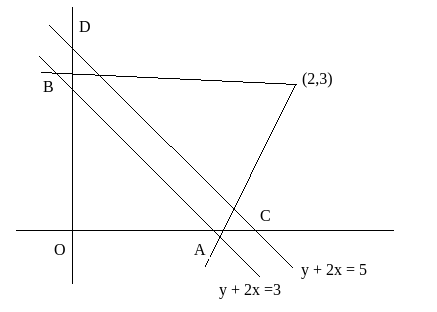
\includegraphics[width=\columnwidth]{fig.png}
 \caption{}
 \label{}
 \end{figure}

\newpage
\item Show that all chords of the curve  $2x^2-y^2-2x+4y=0$. Which subtend a right angle at the origin. Passes through a fixed point. Find the coordinates of the point.(1991)\\
\item Determine all values of a for which the point $(a, a^2)$ lies inside the triangle formed by the lines\\
\begin{align}
 &2x+3y-1 =0 \\
 &x+2y-1 =0 \ \: (1992)\\
 &5x-6y-1 =0 
\end{align}

\item Tangent at a point $\vec{P_1}$ [other than (0,0)] on the curve $y-x^3$ meets the curve again at $\vec{P_2}$. The tangent at $\vec{P_1}$ meets the curve at $\vec{P_2}$ and so on. Show that the abscissae of $\vec{p_1+p_2+p_3+.....+p_n}$ form a G.P. Also find the ratio.(1993)\\
\item A line through $\vec{A}(5,4)$ meets the line $x+3y+2=0$ $2x+y+4=0$ and $x-y-5=0$ at points B,C and D respectively. If    $\frac{15}{AB}^2+\frac{10}{AC}^2-\frac{6}{AD}^2$, find the equation of the line.(1993)\\
\item A triangle PQRS has it's side PQ parallel to the line $y-mx$ and vertices P,Q and S on the lines $y-a$,$ x-b$ and $x--b$, respectively find the locus of the vertex R. (1996)\\
\item Using co-ordinate geometry prove that the three altitudes of any triangle are concurrent (1998)\\
\item For points $P=(x_1,Y_1)$ and $Q=(x_2,y_2)$ of the coordinate palne, a new distance $d(P,Q)$ is defined by $d(P,Q)=\mid x_1-x_2\mid + \mid y_1-y_2\mid$. Let $\vec{O}=(0,0)$  and $\vec{A}=(3,2)$. Prove that the set of points in the first quadrant which are equidistance (with to line new distance) from O and A consists of the union of line segment of finite length and an infinite ray. Sketch this set in a labelled diagram. (2000)\\
\item Let ABC and PQR be any two triangles in the same plane. Assume that the perpendicular from the points A,B,C to the sides QR, RP, PQ respectively are concurrent. Using vector methods or otherwise, prove that the perpendiculars from P,Q,R to BC, CA, AB  respectively are also concurrent. (2000)\\
\item Let a,b,c are real numbers with $a^2+b^2+c^2=1$. Show that the equation\\ 
$\begin{vmatrix}
 ax-by-c & bx+ay   & cx+a\\
 bx+ay   & ax+by-c & cy+b\\
 cx+a    & cy+b    & ax-by+c
\end{vmatrix}$ \\
represents a straight line.    (2001)
\item A straight line L through the origin meets the lines $x+y+1$ and $x+y=3$ at P and Q respectively. Through  P and Q two straight lines $\vec{L_1} and \vec{L_2}$ intersects at R . Show that the locus of R, as L varies, is a staight line. (2002)\\
\item A straight line negative slope passes through the points $(8,2)$ cuts the positive 
coordnate axes at points P and Q. Find the absolute minimum value of $\vec{OP}+\vec{OQ}$, as L varies . Where O is the origin. (2002)\\
\item The area of the triangle formed by the intersection of a line parallel to x-axis and passing through $\vec{p}(h,k)$ with the lines $y-x$ and $x+y-2$ is $4h^2$. Find the locus of the point. (2002)\\
\end{enumerate}

\section*{H   : Assertion and Reason Type Questions}

\begin{enumerate}
\item Lines $L_1: Y-X=0$ and $L_2 :2x+y=0$ intersects the line $L_3:y+2=0$ at P and Q, respectively. The bisector of the acute angle between $L_1 and L_2$ intersects $L_3$ at R.\\
STATEMENT-1 : The ratio $PR:RQ$equals $\sqrt[2]{2}:\sqrt{5}$. because \\
STATEMENT-2 :In any triangle, bisector of an angle divides the triangle into two triangles. (2007)
\begin{enumerate}
\item Statement-1 is True, Statement-2 is True;Satement-2 is not a correct explaination for Statement-1
\item Statement-1 is True, Statement-2 is True;Satement-2 is NOT a correct explaination for Statement-1
\item Statement-1 is True, Statement-2 is False
\item Statement-1 is False, Statement-2 is True
\end{enumerate}
\end{enumerate}

\section*{I    :     Integer Value Correct Type }
\begin{enumerate}
\item For a point P in the plane, let $\vec{d_1}(p)$ and $\vec{d_2}(p)$ be the distance of a point P
from the lines $x-y=0$ and $x=y=0$ respectively. The area of the region R consistes of all points P lying in the first quadrant of the plane and satisfying $2\leq \vec{d_1}(p)+\vec{d_2}(p)\leq$, is (JEE Adv. 2014)
\end{enumerate}

\section*{Section-B   [JEE Main/AIEE]}
\begin{enumerate}
\item A triangle with vertices $(4,0),(-1,-1 ),(3,5)$ is (2002)
\begin{enumerate}
\item isoscales and right angled
\item isoscales  but not right angled
\item right angled but not isoscales 
\item neither right angled nor isoscales 
\end{enumerate}
\item Locus of mid point of the portion between the axes of $x\cos\alpha+y\sin\alpha=p$. Where p is constant is. (2002)
\begin{enumerate}
\item $x^2+y^2=\frac{4}{p^2}$ 
\item $x^2+y^2=4p^2$
\item$\frac{1}{x^2}+\frac{1}{y^2}=\frac{2}{p^2}$ 
\item $\frac{1}{x^2}+\frac{1}{y^2}=\frac{4}{p^2}$ 
\end{enumerate}
\item If the pair of lines $ax^2+2hxy+by^2+2gx+2fy+c=0$ intersects on the y-axis then (2002)
\begin{enumerate}
\item $2fgh=bg^2+ch^2$ 
\item $bg^2\neq ch^2$
\item $abc=2fgh$
\item none of these
\end{enumerate}
\item The pair of lines represented by $3ax^2+5xy+(a^2-2)y^2=0$ are perpendicular to each other for (2002)
\begin{enumerate}
\item two values of a 
\item $\forall a$
\item for one value of a 
\item for no values of a
\end{enumerate}
\item A square of side a lies above the x-axis and has one vertex at the origin. The side passing through the origin makes an angle $\alpha \left[ 0<a<\frac{\Pi}{4}]\right]$ with the positive direction of x-axis. The equation of it's diagonal passing through the origin is (2003)
\begin{enumerate}
\item $y\brak{\cos\alpha+\sin\alpha}+x\brak{\cos\alpha-\sin\alpha}$=a
\item $y\brak{\cos\alpha-\sin\alpha)-x(\sin\alpha-\cos\alpha}$=a
\item $y\brak{\cos\alpha+\sin\alpha)+x(\sin\alpha-\cos\alpha}$=a
\item $y\brak{\cos\alpha+\sin\alpha)+x(\sin\alpha+\cos\alpha}$=a
\end{enumerate}
\item If the pair of straight lines $x^2-2pxy-y^2=0$ and $x^2-2qxy-y^2=0$ be such that each pair bisects the angle between the other pair, then (2003)
\begin{enumerate}
\item $pq=-1$  
\item $p=q$ 
\item $p=-q$  
\item $pq=1$
\end{enumerate}
\item Locus of centroid of the triangle whose vertices are $(a\cos t, a\sin t)$, $(a\sin t,-b\cos t)$ and (1,0) where t is a parameter, is (2003)
\begin{enumerate}
\item $(3x+1)^2+(3y)^2=a^2-b^2$
\item $(3x-1)^2+(3y)^2=a^2-b^2$
\item $(3x-1)^2+(3y)^2=a^2+b^2$
\item $(3x+1)^2+(3y)^2=a^2+b^2$
\end{enumerate}
\item If $x_1,x_2,x_3$ and $y_1,y_2,y_3$ are both in G.P with the same common ratio then the points $(x_1,y_1),(x_2,y_2)$ and $(x_3,y_3)$ (2003)
\begin{enumerate}
\item are vertices of a triangle
\item lies on a straight line
\item lies on ellipse
\item lies on circle
\end{enumerate}
\item If the equation of the locus of a equidistance from the point $(a_1,b_1)$ and $(a_2,b_2)$ is $(a_1-b_2)x+(a_1-b_2)y+c=0$, then the value of 'c' is (2003)
\begin{enumerate}
\item $\sqrt{a_1^2+b_1^2-a_2^2-b_2^2}$
\item $\frac{1}{2}(a_2^2+b_2^2-a_1^2-b_1^2)$
\item $a+1^2-a_2^2+b_1^2-b_2^2$
\item $\frac{1}{2}(a_1^2+a_2^2+b_1^2+b_2^2)$
\end{enumerate}
\item Let $\vec{A}(2,-3)$ and $\vec{B}(-2,3)$ be vertices of a triangle ABC. If the centroid of this triangle moves on the line $2x+3y=1$, then the locus of the vertex C is in the line  (2004)
\begin{enumerate}
\item $3x-2y=0$
\item $2x-3y=7$ 
\item $3x+2y=5$ 
\item $2x+=3y=9$
\end{enumerate}
\item The equation of the straight line passing through the point $(4,3)$ and making intercepts on the coordinate axes whose sum is -1 is (2004)
t\begin{enumerate}
\item $\frac{x}{2}-\frac{y}{3}=1$ and $\frac{x}{-2}+\frac{y}{1}=1$
\item $\frac{x}{2}-\frac{y}{3}=-1$ and $\frac{x}{-2}+\frac{y}{1}=-1$
\item $\frac{x}{2}+\frac{y}{3}=1$ and $\frac{x}{2}+\frac{y}{1}=1$
\item $\frac{x}{2}+\frac{y}{3}=1$ and $\frac{x}{-2}+\frac{y}{1}=-1$
\end{enumerate}
\item If the sum of the slopes of the lines given by $x^2-2cxy-7y^2=0$ is four times the product c has the value (2004)
\begin{enumerate}
\item -2 
\item -1 
\item  2 
\item  1
\end{enumerate}
\item If one of the lines given by $6x^2-xy+4cy^2=0$ is $3x+4y=0$, then c equals (2004)
\begin{enumerate}
\item -3 
\item -1 
\item  3 
\item  1
\end{enumerate}
\item The line parallel to the x-axis and passing through the intersection of the lines $ax+2by+3b=0$ and $bx-2ay-3a=0$, where $(a,b) \neq (0,0)$ (2005)
\begin{enumerate}
\item below the x-axis at a distance of $\frac{3}{2}$ from it
\item below the x-axis at a distance of $\frac{2}{3}$ from it
\item above the x-axis at a distance of $\frac{3}{2}$ from it
\item above the x-axis at a distance of $\frac{2}{3}$ from it
\end{enumerate}
\item If a vertex of a triangle is (1,1) and the mid point of two sides of this vertex are (-1,2) and (3,2) then the centroid of the triangle is (2005)
\begin{enumerate}
\item $\sbrak{-1,\frac{7}{3}}$ 
\item $\sbrak{\frac{-1}{3},\frac{7}{3}}$ 
\item $\sbrak{1,\frac{7}{3}}$  
\item $\sbrak{\frac{1}{3},\frac{7}{3}}$ 
\end{enumerate}
\item A straigjt line through point $A(3,4)$ is such that it's intercept between the axes is bisected at A. It's equation is (2006)
\begin{enumerate}
\item $x+y=7$ 
\item $3x-4y+7=0$  
\item $4x+3y=24$ 
\item $3x+4y=25$
\end{enumerate}
\item If $(a,a^2)$ falls inside the angle made by the lines $y= \frac{x}{2}, x>0$ and $y=3x, x>0$, then a belong to (2006)
\begin{enumerate}
\item $\sbrak{0,\frac{1}{2}}$ 
\item $(3,\infty)$ 
\item $\sbrak{\frac{1}{2},3}$ 
\item $\sbrak{-3,\frac{1}{2}}$
\end{enumerate}
\item Let $\vec{A}(h,k)$ and $\vec{B}(1,1)$ and $\vec{C}(2,1)$ be the vertices of a right angle triangle with AC as it's hypotenuse. If the area of the triangle is 1 square unit, then the set of values which 'k' can taken is given by (2007)
\begin{enumerate}
\item $(-1,3)$ 
\item $(-3,-2)$
\item $(1,3)$ 
\item $(0,2)$
\end{enumerate}
\item Let $\vec{P}=(-1,0),\vec{Q}=(0,0) and \vec{R}=(3,\sqrt[3]{3})$ be three points. The equation of the bisector of the angle PQR is (2007)
\begin{enumerate}
\item $\frac{\sqrt{3}}{2}x+y=0$ 
\item $x+\sqrt{3}y=0$ 
\item $\sqrt{3}x+y=0$ 
\item $x+\frac{\sqrt{3}}{2}y=0$.
\end{enumerate}
\item If one of the lines of $my^2+(1-m^2)xy-mx^2=0$ is a bisector of the angle between the lines $xy=0$, then m is (2007)
\begin{enumerate}
\item 1  
\item 2 
\item $\frac{-1}{2}$ 
\item -2
\end{enumerate}
\item The perpendicular bisector of the line segment joining $P(1,4)$ and $Q(k,3)$ has y-intercept -4. Then a possible value of k is (2008)
\begin{enumerate}
\item  1 
\item  2 
\item -2 
\item -4
\end{enumerate}
\item The shortest distance between the line $y-x=1$ and the curve $x=y^2$ is (2009)
\begin{enumerate}
\item $\frac{\sqrt{2}{3}}{8}$ 
\item $\frac{\sqrt{3}{2}}{5}$ 
\item $\frac{\sqrt{3}}{4}$ 
\item $\frac{\sqrt{3}{2}}{8}$.
\end{enumerate}
\item The lines $p(p^2+1)x-y+q=0$ and $(p^2+1)^2x+(p^2+1)y+2q=0$ are perpendicular to a common line for (2009)
\begin{enumerate}
\item exactly one value of p
\item exactly two values of p
\item more than two values of p
\item no value of p
\end{enumerate}
\item Three distinct points A,B and C are given i the 2-dimentional coordinates plane such that the ratio of the  distance of any one of them from the point (1,0) to the distance from the point (-1,0) is equal to $\frac{1}{3}$. Then the circumcenter of the triangle ABC is at the point; (2009)
\begin{enumerate}
\item $\sbrak{\frac{5}{4} ,0}$ 
\item $\sbrak{\frac{5}{2} ,0}$ 
\item $\sbrak{\frac{5}{3} ,0}$
\item (0,0)
\end{enumerate}
\item The line L given by $\frac{x}{5}+\frac{y}{b}=1$ passes through the point (13,32). The line K is parallel L and has the equation $\frac{x}{c}+\frac{y}{3}=1$. Then the distance between L and K is. (2010)
\begin{enumerate}
\item $\sqrt{17}$  
\item $\frac{17}{\sqrt{15}}$ 
\item $\frac{23}{\sqrt{17}}$ 
\item $\frac{23}{\sqrt{15}}$
\end{enumerate}
\item The line $L_1:y-x=0$ and $L_2: 2x+=y=0$ intersects the line $L_3: y+2=0$ at P and Q respectively. The bisector of the acute angle between $L_1 and L_2$ intersects $L_3$ at R 
STATEMENT-1: The ratio PR:RQ equals $\sqrt[2]{2}:\sqrt{5}$\\
STATEMENT-2: In any triangle,bisector of an angle divides the triangle into two similar triangles.(2011)
\begin{enumerate}
\item Statement-1 is True, Statement-2 is True,Statement-2 is not a correct explaination for the Statement-1.
\item Statement-1 is True, Statement-2 is False
\item Statement-1 is False, Statement-2 is True
\item Statement-1 is True, Statement-2 is True, tatement-2 is correct explaination for the Statement-1.
\end{enumerate}
\item If the line $2x +y=k$ passes through the point which divides the line segment joining the points $(1,1)$ and (2,4) in the ratio $3:2$,then k equals: (2012)
\begin{enumerate}
\item $\frac{29}{5}$ 
\item 5 
\item 6 
\item $\frac{11}{5}$
\end{enumerate}
\item A ray of light along $x+\sqrt{3}y=\sqrt{3}$ get reflected upon reaching x-axis, the equation of the reflected ray is (JEE M 2013)
\begin{enumerate}
\item $y=x+\sqrt{3}$ 
\item $\sqrt{3}y=x-\sqrt{3}$ 
\item $y=\sqrt{3}x-\sqrt{3}$ 
\item $\sqrt{3}y=x-1$ 
\end{enumerate}
\item The coordinate of the incenter of the triangle that has the coordinates of mid points of it's sides as (0,1) (1,1) and (1,0) is; (JEE M 2013)
\begin{enumerate}
\item $2+\sqrt{2}$
\item $2-\sqrt{2}$ 
\item $1+\sqrt{2}$ 
\item $1-\sqrt{2}$
\end{enumerate}
\item Let PS e the median of the triangle with vertices $\vec{P}(2,2)$,$\vec{Q}(6,-1)$ and $\vec{R}(7,3)$. The equation of the line passing through (1,-1)and parallel to PS is: (JEE M 2014)
\begin{enumerate}
\item $4x+7y+3=0$ 
\item $2x-9y+11=0$ 
\item $4x-7y+11=0$ 
\item $2x+7y+9=0$ 
\end{enumerate}
\item Let a,b,c and d be non-zero numbers. If the point of intersection of the lines $4ax+2ay+c=0$ and $5bx+2by+d=0$ lies in the fourth quadrant and eqidistance from the two axes then (JEE M 2014)
\begin{enumerate}
\item $3bc_2ad=0$  
\item $3bc+2ad=0$
\item $2b-3ad=0$ 
\item $2bc+3ad=0$
\end{enumerate}
\item The number of points, having both co-ordinates as integers, that lie in the interior of the triangle ith vertices (0,0)(0,41) and(41,0)is. (JEE M 2015)
\begin{enumerate}
\item 820 
\item 780 
\item 901 
\item 861
\end{enumerate}
\item Two sides  of a rhombus are alone the lines, $x-y+1=0$ and $7x+y-5=0$. If it's diagoals intersect at(-1,-2), then which one of the following is a vertex of this rhombus? (JEE M 2016)
\begin{enumerate}
\item $\brak{\frac{1}{3},\frac{8}{3}}$ 
\item $\brak{\frac{10}{3},\frac{7}{3}}$ 
\item $\brak{-3,-9}$ 
\item $\brak{-3,-8}$
\end{enumerate}
\item A straight the thrugh a fixed point (2,3)intersects the coordinate axes at distinct point P  and Q. If O is the origin and the rectangle OQPR is completed, then the locus of R is: (JEE M 2018)
\begin{enumerate}
\item $2x+3y=xy$ 
\item $3x+2y=xy$ 
\item $3x+2y=6xy$ 
\item $3x+2y=6$
\end{enumerate}
\item consider the set of all lines $px+qy+r=0$ such that $3p+2q+4r=0$. Which one of the following statements is true? [JEE M 2019-9 Jan (M)]
\begin{enumerate}
\item The lines are concurent at the point $\brak{\frac{3}{4},\frac{1}{2}} $.
\item Each the line passes through the origin.
\item The lines are parallel.
\item The lines are not concurrent.
\end{enumerate}
\item Slope of line passing through $P(2,3)$ and intersecting the line $x+y=7$ at a distance of 4 units from  P,  is : [JEE M 2019-9 April (M)]
\begin{enumerate}
\item $\frac{1-\sqrt{5}}{1+\sqrt{5}}$
\item $\frac{1-\sqrt{7}}{1+\sqrt{7}}$
\item $\frac{\sqrt{7}-1}{\sqrt{7}+1}$
\item $\frac{\sqrt{5}-1}{\sqrt{5}+1}$
\end{enumerate}
\end{enumerate}
\end{document}
\chapter{Three Dimensional Geometry}
\iffalse
\documentclass[12pt]{article}
\usepackage{graphicx}
\usepackage{enumerate}
\usepackage{amsmath}
\usepackage{ragged2e}
\usepackage{listings}
\newenvironment{matchtabular}{%
  \setcounter{matchleft}{0}%
  \setcounter{matchright}{0}%
  \tabularx{\textwidth}{%
    >{\leavevmode\hbox to 1.5em{\stepcounter{matchleft}\arabic{matchleft}.}}X%
    >{\leavevmode\hbox to 1.5em{\stepcounter{matchright}\alph{matchright})}}X%
    }%
}{\endtabularx}

%\usepackage{blindtext}
\usepackage{multicol}
\title{Multicols Demo}
\setlength{\columnsep}{3cm}
\usepackage{tabularx}
 \usepackage[utf8]{inputenc}
\newcounter{matchleft}
\newcounter{matchright}

\newcommand*{\vv}[1]{\vec}
\newcommand{\myvec}[1]{\ensuremath{\begin{pmatrix}#1\end{pmatrix}}}
\newcommand{\mydet}[1]{\ensuremath{\begin{vmatrix}#1\end{vmatrix}}}
\providecommand{\brak}[1]{\ensuremath{\left(#1\right)}}
\providecommand{\lbrak}[1]{\ensuremath{\left(#1\right.}}
\providecommand{\rbrak}[1]{\ensuremath{\left(#1\right)}}
\providecommand{\sbrak}[1]{\ensuremath{{}\left[#1\right]}}
%\let\vec\mathbf

\begin{document}
\begin{center}
\textbf\large{CHAPTER-20 \\ Vector Algebra and
 Three Dimensional Geometry}

\end{center}
\fi
\section*{Section-A    [JEE Advanced/IIT-JEE]}
\section*{A    :  Fill in the Blanks}
\begin{enumerate}
\item Let $\vec{A},\vec{B},\vec{C}$ be vectors of length 3,4,5 respectively. Let $\vec{A}$ perpendicular to $\vec{B}+\vec{C},\vec{B}$ to $\vec{C}+\vec{A}$ and $\vec{C}$ to $\vec{A}+\vec{B}$. Then  the length of vector $\vec{A+B+C}$ is......     (1981)
\item The unit vector perpendicual to plane determined by $P(1,-1,2),Q(2,0,-1) and R(0,2,1)$is.....     (1983)
\item The area of whose vertices are $A(1,-1,2),B(2,1,-1)C(3,-1,2)$ is.....(1983)
\item A,B,C and D are four points in a plane with position vectors a,b,c and d respectively such that   $\brak{\vec{a}-\vec{d}}\brak{\vec{b}-\vec{c}}=\brak{\vec{b}-\vec{d}}\brak{\vec{c}-\vec{a}}$   (1984)\\
The point D then,is the.......... of the triangle ABC.
\item If$\begin{vmatrix}
 a & a^2 & 1+a^3\\
 b & b^2 & 1+b^3\\
 c & c^2 & 1+c^3
\end{vmatrix}$ \\ =0 and the vectors $\vec{A}=(1,a,a^2)$, $\vec{B}=(1,b,,b^2)$, $\vec{C}=(1,c,c^2)$, are non-coplanar, then the product abc =..........(1984)
\item If $\vec{a}, \vec{b}, \vec{c}$ are three non-coplanar vectors, then-$\frac{\vec{A}\cdot\vec{B}\times\vec{C}}{\vec{C}\times\vec{A}\cdot\vec{B}}+\frac{\vec{B}\cdot\vec{A}\times\vec{C}}{\vec{C}\cdot\vec{A}\times\vec{B}}$ =..........(1985)
\item If the vectors $a\hat{i}+\hat{j}+\hat{k}$, $\hat{i}+b\hat{j}+\hat{k}$ and $\hat{i}+\hat{j}+c\hat{k}$, $(a\neq b\neq c\neq 1)$ are coplanar, hen the value of $\frac{1}{1-a}$+$\frac{1}{1-b}$+$\frac{1}{1-c}$ =..........(1987)
\item Let $b=4\hat{i}+3\hat{j}$ and $\vec{c}$ be two vectors perpendicular to each other in the xy-plane. All vectors n the same plane having projections 1 and 2 along $\vec{b} and \vec{c}$,respectively are given by ........(1987)
\item The components of a vector $\vec{a}$ along and perpendicular t a non zero vector $\vec{b}$ are.....and.....respectively.  (1988)
\item Given that $\vec{a}=(1,1,1)\vec{c}=(0,1,-1),\vec{a}\vec{b}=3$ and $\vec{a}\times\vec{b}=\vec{c}$, ten $\vec{b}$=........(1991)
\item A unit vector coplanar with $\vec{i}+\vec{j}+2\vec{k}$ and $\vec{i}+2\vec{j}=\vec{k}$ and perpendicular to $\vec{i}+\vec{j}+\vec{k}$ is.......(1992)
\item A unit vector perpendicular to the plane determined by the points $P(1,-1,2),Q(2,0,-1) and R(0,2,1)$ is.....(1994) 
\item A nonzero vector $\vec{a}$ is parallel to the line of intersection of the plane determined by the vectors $\hat{i},\hat{i}+\hat{j}$ and the plane determined by the vectors $\hat{i}-\hat{j},\hat{i}+\hat{k}$. The angle between $\vec{a}$ and the vector $\hat{i}-2\hat{j}+2\hat{k}$  is........(1996)
\item If $\vec{b}$ and $\vec{c}$ are any two nn collinear unit vectoers and $\vec{a}$ is any vector then $\brak{\vec{a}\cdot\vec{b}}\vec{b}+\brak{\vec{a}\cdot\vec{c}}\vec{c}$+$\frac{\vec{a}\cdot \brak{\vec{b}\times\vec{c}}}{\mid\vec{b}\times\vec{c}\mid}$ $\brak{\vec{b}\times \vec{c}}$=..........(1996)
\item Let $OA=a, OB=10a+2b$ and $OC=b$ where O,A and C are non collinear points. Let P denote the are of the qudrailateral OABC, and let q denote the area of the parallelogram  with OA and OC as adjacent sides. IfP=kq, then K=...........(1997) 
\end{enumerate}

\section*{B    :    True/False}

\begin{enumerate}
\item $\vec{A},\vec{B}$ and $\vec{C}$  be unit vectors suppose that $\vec{A}\cdot\vec{B}=\vec{A}\cdot\vec{C}=0$, and that the angle between $\vec{B} and \vec{C}$ is $\frac{\pi}{6}$. Then $\vec{A}=+-2\brak{\vec{B\times\vec{C}}}$.    (1981)
\item If $X\cdot A=0,X\cdot B=0. X\cdot C=0$ for some non-zero vectors X, then [A B C]=0(1983)
\item The points with position vectors $a+b,a-b and a+kb$ are collinear for all real values of k.   (1984)
\item For any three vectors $\vec{a},\vec{b}$ and $\vec{c}$,$\brak{\vec{a}-\vec{b}}$
$\cdot$ $\brak{\vec{b}-\vec{c}}$ $\times$ $\brak{\vec{c}-\vec{a}}$ =$2\vec{a}\cdot\vec{b}\times\vec{c}$
\end{enumerate}

\section*{C  :   MCQ'S with One Correct Answer}

\begin{enumerate}
\item The scalar $\vec{A}\cdot\brak{\vec{B}+\vec{C}}\times\brak{\vec{A}+\vec{B}+\vec{C}}$ equals: (1981)
\begin{enumerate}
\item 0
\item $\sbrak{\vec{A} \vec{B} \vec{C}}$+$\sbrak{\vec{B} \vec{C} \vec{A}}$
\item $\sbrak{\vec{A} \vec{B} \vec{C}}$
\item None of these
\end{enumerate}
\item For non-zero vectors $\vec{a},\vec{b},\vec{c},\mid\brak{\vec{a}\times\vec{b}}\cdot\vec{c}\mid$=$\mid\vec{a}\mid \mid\vec{b}\mid \mid\vec{c}\mid$ holds if and only if        (1982)
\begin{enumerate}
\item $\vec{a}\cdot\vec{b}=0$,$\vec{b}\cdot\vec{c}=0$
\item $\vec{b}\cdot\vec{c}=0$,$\vec{c}\cdot\vec{a}=0$
\item $\vec{c}\cdot\vec{a}=0$,$\vec{a}\cdot\vec{b}=0$
\item $\vec{a}\cdot\vec{b}=\vec{b}\cdot\vec{c}=\vec{c}\cdot\vec{a}=0$
\end{enumerate}
\item The volume of the parallelopiped whose sides are given by $\overrightarrow{OA}=2i-2j$,$\overrightarrow{OB}=i+j-k$,$\overrightarrow{OC}=3i-k$, is (1983)
\begin{enumerate}
\item $\frac{4}{13}$
\item 4
\item $\frac{2}{7}$
\item None of these
\end{enumerate}
\item The two points with positiooning vectors $60+3j,40i-8j,ai-52j$ are colinearr if (1983)
\begin{enumerate}
\item a=-40
\item a=40
\item a=20
\item  None of these
\end{enumerate}
\item Let $\vec{a},\vec{b},\vec{c}$ be three non-coplanar vectors and $\vec{p},\vec{q},\vec{r}$ are vectors defined by the relations $\vec{p}=\frac{\vec{b}\times\vec{c}}{\sbrak{\vec{a}\cdot\vec{b}\cdot\vec{c}}}$,$\vec{q}=\frac{\vec{c}\times\vec{a}}{\sbrak{\vec{a}\cdot\vec{b}\cdot\vec{c}}}$,$\vec{r}=\frac{\vec{a}\times\vec{b}}{\sbrak{\vec{a}\cdot\vec{b}\cdot\vec{c}}}$ then the value of the expression $\brack{\vec{a}+\vec{b}}\cdot\vec{p}$+$\brack{\vec{b}+\vec{c}}\cdot\vec{q}$+$\brack{\vec{c}+\vec{a}}\cdot\vec{r}$ is equal to    (1988)
\begin{enumerate}
\item 0
\item 1
\item 2
\item 3
\end{enumerate}
\item Let be distinct non-negative numbers. If the vectors $a\hat{i}+a\hat{j}+c\hat{k},\hat{i}+\hat{k}$ and $c\hat{i}+c\hat{j}+b\hat{k}$ lie in a plane, then c is  (1993)
\begin{enumerate}
\item The Arithmetic Mean of a and b
\item The Geometric Mean of a and b
\item The Harmonic Mean of a and b
\item equal to zero
\end{enumerate}
\item Let $\vec{P}$ and $\vec{Q}$ are position vectors of P and Q respectively, with respect to O and $\vec{p}=p,\vec{q}=q$. The points R and S divide PQ internally and externally in the ratio $2:3$ respectively. If OR and OS are perpendicular then (1994)
\begin{enumerate}
\item $9q^2=4q^2$
\item $4p^2=9q^2$ 
\item $9p=4q$
\item $4p=9q$
\end{enumerate}
\item Let $\alpha,\beta,\gamma $ be distinct real numbers. The point with position vectors $\alpha\hat{i}+\beta\hat{j}+\gamma\hat{k},\beta\hat{i}+\gamma\hat{j}+\alpha\hat{k},\gamma\hat{i}+\alpha\hat{j}+\beta\hat{k}$      (1994)
\begin{enumerate}
\item are collinear 
\item from an equilateral triangle
\item from a scalene triangle
\item from a right angled triangle
\end{enumerate}
\item Let $\vec{a}=\hat{i}-\hat{j},\vec{b}=\hat{j}-\hat{k},\vec{c}=\hat{k}-\hat{i}$. If $\vec{d}$ is a unit vector such that $\vec{a}\cdot\vec{d}=0=\sbrak{\vec{b} \vec{c} 
\vec{d}}$,then $\vec{d}$ equals (1995)
\begin{enumerate}	
\item $\pm\frac{\hat{i}+\hat{j}-2\hat{k}}{\sqrt{6}}$
\item $\pm\frac{\hat{i}+\hat{j}-\hat{k}}{\sqrt{3}}$
\item $\pm\frac{\hat{i}+\hat{j}+\hat{k}}{\sqrt{3}}$
\item $\pm\hat{k}$
\end{enumerate}
\item If $\vec{a},\vec{b},\vec{c}$ are non coplanar unit vectors such that $\vec{a}\times\brak{\vec{b}\times\vec{c}}$=$\frac{\brak{\vec{b}+\vec{c}}}{\sqrt{2}}$, then the angle between $\vec{a}$ and $\vec{b}$ is  (1995)
\begin{enumerate}	
\item $\frac{3\pi}{4}$
\item $\frac{\pi}{4}$
\item $\frac{\pi}{2}$
\item $\pi$
\end{enumerate}
\item Let $\vec{u},\vec{v}$ and $\vec{w}$ be vectors such that $\vec{u}+\vec{v}+\vec{w}=0$. If $\mid\vec{u}\mid=3,\mid\vec{v}\mid=4,\mid\vec{w}\mid=5$, then $\vec{u}\cdot\vec{v}+\vec{v}\cdot\vec{w}+\vec{w}\cdot\vec{u}+$ is
\begin{enumerate}	
\item 47
\item -25
\item 0
\item 25
\end{enumerate}
\item If $\vec{a},\vec{b}$ and $\vec{c}$  are three non coplanar vectors, then $\brak{\vec{a}+\vec{b}+\vec{c}}\cdot\sbrak{\brak{\vec{a}+\vec{b}}\times\brak{\vec{a}+\vec{c}}}$ equals  (1995)
\begin{enumerate}	
\item 0
\item $\sbrak{\vec{a} \vec{b} \vec{c}}$
\item $2\sbrak{\vec{a} \vec{b} \vec{c}}$
\item $-\sbrak{\vec{a} \vec{b} \vec{c}}$
\end{enumerate}
\item Let $a=2i+j-2k, b=i+j$. If c is a vector such that a. $c=\mid c \mid, \mid c-a \mid =\sqrt[2]{2}$ and the angle between $\brak{a \times b}$ and c is $30\circ$ then $\mid\brak{a \times b}\times c \mid$=   (1999)
\begin{enumerate}	
\item $\frac{2}{3}$
\item $\frac{3}{2}$
\item 2
\item 3
\end{enumerate}
\item Let $a=2i+j+k, b=i+2j-k$ and a unit vector c be coplanar. If c is perpendicular to a, then c =     (1999)
\begin{enumerate}
\item $\frac{1}{\sqrt{2}} \brak{-j+k}$  
\item $\frac{1}{\sqrt{3}} \brak{-i-j-k}$   
\item $\frac{1}{\sqrt{5}} \brak{i-2j}$  
\item $\frac{1}{\sqrt{3}} \brak{i-j-k}$  
\end{enumerate}
\item If the vectors $\vec{a},\vec{b}$ and $\vec{c}$ from the sides BC,CA and AB respectivelly of a triangle ABC, then   (2000)
\begin{enumerate}	
\item $\vec{a}\cdot\vec{b}+\vec{b}\cdot\vec{c}+\vec{c}\cdot\vec{a}=0$
\item $\vec{a}\times\vec{b}=\vec{b}\times\vec{c}=\vec{c}\times\vec{a}$
\item $\vec{a}\cdot\vec{b}=\vec{b}\cdot\vec{c}=\vec{c}\cdot\vec{a}$
\item $\vec{a}\times\vec{b}+\vec{b}\times\vec{c}+\vec{c}\times\vec{a}=0$
\end{enumerate}
\item Let the vectors $\vec{a},\vec{b}, \vec{c}$ and $\vec{d}$ be such that $\brak{\vec{a}\times\vec{b}}\times\brak{\vec{c}\times\vec{d}}=0$. Let $p_1 and P_2$ be planes determined by the pairs of vectors  $\vec{a},\vec{b}$ and $\vec{c}, \vec{d}$ respectvely. Then the angle between $p_1 and P_2$  is (2000)
\begin{enumerate}	
\item  0 
\item  $\frac{\pi}{4}$
\item  $\frac{\pi}{3}$
\item  $\frac{\pi}{2}$
\end{enumerate}
\item If $\vec{a},\vec{b}$ and $\vec{c}$ are unit coplanar vectors, then the scalar triple product $\sbrak{2\vec{a}-\vec{b},2\vec{b}-\vec{c},2\vec{c}-\vec{a}}=$  (2000)
\begin{enumerate}	
\item 0
\item 1
\item -$\sqrt{3}$
\item  $\sqrt{3}$
\end{enumerate}
\item Let $\vec{a}=\vec{i}-\vec{k},\vec{b}=x\vec{i}+\vec{j}+\brak{1-x}\vec{k}$ and $\vec{c}=y\vec{i}+x\vec{j}+\brak{1+x-y}\vec{k}$. Then $\sbrak{\vec{a}\vec{b}\vec{c}}$ depends on (2000)
\begin{enumerate}	
\item only x
\item only y
\item neither x nor y
\item both x and y
\end{enumerate}
\item If $\vec{a},\vec{b}$ and $\vec{c}$ are unit vectors, then $\mid \vec{a}-\vec{b}\mid^2 +\mid \vec{b}-\vec{c}\mid^2+\mid \vec{c}-\vec{a}\mid^2 $ dose NOT exceed (2001)
\begin{enumerate}	
\item 4
\item 9
\item 8 
\item 6
\end{enumerate}
\item If $\vec{a} and \vec{b}$ are two unit vectors such that $\vec{a}+2\vec{b}$ and $5\vec{a}-4\vec{b}$ are perpendicular to each other then the angle between $\vec{a}$ and $\vec{b}$ is (2002)
\begin{enumerate}	
\item $45\circ$
\item $60\circ$
\item $\cos^{-1}\frac{1}{3}$
\item $\cos^{-1}\frac{2}{7}$
\end{enumerate}
\item Let $\vec{V}=2\vec{i}+\vec{j}-\vec{k}$ and $\vec{W}=\vec{i}+3\vec{k}$. If $\vec{U}$ is a unit vector, then the maxium value of the scalar triple product $\mid\vec{V}\vec{V}\vec{W}\mid$ is (2002)
\begin{enumerate}	
\item -1
\item $\sqrt{10}+\sqrt{6}$
\item $\sqrt{59}$
\item $\sqrt{60}$
\end{enumerate}
\item The value of K such that $\frac{x-4}{1}=\frac{y-2}{1}=\frac{z-k}{2}$ lies in the plane $2x-4y+z=7$, is   (2003)
\begin{enumerate}	
\item 7
\item -7
\item no real value
\item 4
\end{enumerate}
\item The value of 'a' such that the volume of parallelopiped formed by $\hat{i}+a\hat{j}+\hat{k},\hat{j}+a\hat{k}$ and $a\hat{i}+\hat{k}$ becomes minimum is (2004)
\begin{enumerate}	
\item -3
\item 3
\item $\frac{1}{\sqrt{3}}$
\item $\sqrt{3}$
\end{enumerate}
\item If $\vec{a}=\brak{\hat{i}+a\hat{j}+\hat{k}\cdot\vec{a}\cdot\vec{b}=1}$ and $\vec{a}\times\vec{b}=\hat{j}-\hat{k}$, then $\vec{b}$ is
\begin{enumerate}
\item $\hat{i}-\hat{j}+\hat{k}$
\item $2\hat{j}-\hat{k}$
\item $\hat{i}$
\item $2\hat{i}$
\end{enumerate}
\item If the lines $\frac{x-1}{2}=\frac{y+1}{3}=\frac{z-1}{4}$ and $\frac{x-3}{1}=\frac{y-k}{2}=\frac{z}{1}$ intersect, then the value of k is
\begin{enumerate}
\item $\frac{3}{2}$
\item $\frac{9}{2}$
\item $\frac{2}{9}$
\item $\frac{3}{2}$
\end{enumerate}
\item The unit vector which is orthogonal to the vector $3\hat{i}+2\hat{j}+6\hat{k}$ and is coplanar with the vectors $2\hat{i}+\hat{j}+\hat{k}$ and $\hat{i}-\hat{j}+\hat{k}$ is
\begin{enumerate}
\item $\frac{2\hat{i}-6\hat{j}+\hat{k}}{\sqrt{41}}$
\item $\frac{2\hat{i}-3\hat{j}}{\sqrt{13}}$
\item $\frac{3\hat{i}-\hat{k}}{\sqrt{10}}$
\item $\frac{4\hat{i}+3\hat{j}-3\hat{k}}{\sqrt{34}}$
\end{enumerate}
\item A variable plane at the distance of the one unit from the origin cuts the coordinates axes at A,B and C. If the centroid $D\brak{x,y,z}$ of triangle ABC satisfies the relation $\frac{1}{x^2}+\frac{1}{y^2}+\frac{1}{z^2}=k$ then the value of k is 
\begin{enumerate}
\item 3
\item 1
\item $\frac{1}{3}$
\item 9
\end{enumerate}
\item If $\vec{a},\vec{b}$ and $\vec{c}$ are three non-zero and non coplanar vectors $\vec{b_1}=\vec{b}-\frac{\vec{b}\cdot\vec{a}}{\mid\vec{a}\mid^2} \vec{a}$, $\vec{b_2}=\vec{b}+\frac{\vec{b}\cdot\vec{a}}{\mid\vec{a}\mid^2} \vec{a}$, $\vec{c_1}=\vec{c}-\frac{\vec{c}\cdot\vec{a}}{\mid\vec{a}\mid^2} \vec{a}$+$\frac{\vec{b}\cdot\vec{c}}{\mid\vec{c}\mid^2}\vec{b_1}$, $\vec{c_2}=\vec{c}-\frac{\vec{c}\cdot\vec{a}}{\mid\vec{a}\mid^2}\vec{a}$-$\frac{\vec{b_1}\cdot\vec{c}}{\mid\vec{b_1}\mid^2}\vec{b_1}$, $\vec{c_3}=\vec{c}-\frac{\vec{c}\cdot\vec{a}}{\mid\vec{c}\mid^2} \vec{a}$+$\frac{\vec{b}\cdot\vec{c}}{\mid\vec{c}\mid^2} \vec{b_1}$, $\vec{c_4}=\vec{c}-\frac{\vec{c}\cdot\vec{a}}{\mid\vec{a}\mid^2} \vec{a}$=$\frac{\vec{b}\cdot\vec{c}}{\mid\vec{b}\mid^2} \vec{b_1}$ then the seet of orthogonal vector is
\begin{enumerate}
\item $\brak{\vec{a}, \vec{b_1}, \vec{c_3}}$
\item $\brak{\vec{a}, \vec{b_1}, \vec{c_2}}$
\item $\brak{\vec{a}, \vec{b_1}, \vec{c_1}}$
\item $\brak{\vec{a}, \vec{b_2}, \vec{c_2}}$
\end{enumerate}
\item A plane which is perpendicular to two planes $2x-2y+z=0$ and $x-y+2z=4$ passes through $\brak{1,-2,1}$. The distance of the plane from the point $\brak{1,2,2}$ is\
\begin{enumerate}
\item 0
\item 1
\item $\sqrt{2}$
\item $\sqrt[2]{2}$
\end{enumerate}
\item Let $\vec{a}=\hat{i}+2\hat{j}+\hat{k},\vec{b}=\hat{i}-\hat{j}+\hat{k}$ and $\vec{c}=\hat{i}+\hat{j}-\hat{k}$ . A vector in the plane of $\vec{a} and \vec{b}$ whose projection on $\vec{c}$ is $\frac{1}{\sqrt{3}}$ is
\begin{enumerate}
\item $4\hat{i}-\hat{j}+4\hat{k}$
\item $3\hat{i}+\hat{j}-3\hat{k}$
\item $2\hat{i}+\hat{j}-2\hat{k}$
\item $4\hat{i}+\hat{j}-4\hat{k}$
\end{enumerate}
\item The number of real distinct values of $\lambda$, for which the vectors $-\lambda^2\hat{i}+\hat{j}+\hat{k},\hat{i}-\lambda^2\hat{j}+\hat{k}$ and $\hat{i}+\hat{j}-\lambda^2\hat{k}$ are coplanar, is
\begin{enumerate}
\item zero 
\item one 
\item two 
\item three
\end{enumerate}
\item Let $\vec{a},\vec{b}$ and $\vec{c}$ are unit vectors such that $\vec{a}+\vec{b}+\vec{c}=\vec{0}$. Which one of the following is correct ?
\begin{enumerate}
\item $\vec{a}\times\vec{b}=b\times\vec{c}=\vec{c}\times\vec{a}=\vec{0}$
\item $\vec{a}\times\vec{b}=b\times\vec{c}=\vec{c}\times\vec{a}\neq\vec{0}$
\item $\vec{a}\times\vec{b}=b\times\vec{c}=\vec{c}\times\vec{c}\neq\vec{0}$
\item $\vec{a}\times\vec{b},b\times\vec{c},\vec{c}\times\vec{a}=\vec{0}$ are mutually perpendicular
\end{enumerate}
\item The edges of the parallelopiped are of unit length and are parallel to non- coplanar unit vectors $\hat{a},\hat{b},\hat{c}$ such that $\hat{a}\cdot\hat{b}=\hat{b}\cdot\hat{c}=\hat{c}\cdot\hat{a}=\frac{1}{2}$. Then the volume of parallelopiped is  (2008)
\begin{enumerate}
\item $\frac{1}{\sqrt{2}}$
\item $\frac{1}{\sqrt[2]{2}}$
\item $\frac{\sqrt{3}}{2}$
\item $\frac{1}{\sqrt{3}}$
\end{enumerate}
\item Let two non-coplanar unit vectors $\hat{a} and \hat{b}$ form an acute  angle. A point P moves so that at any time t the position vector $\overrightarrow{OP}$(here O is the origin) is given by $\hat{a}\cos t+\hat{b}\sin t$. Then P is farthest from origin O,let M be the length of $\overrightarrow{OP}$ and $\hat{u}$ be the unit vector along $\overrightarrow{OP}$. Then, (2008)
\begin{enumerate}
\item $\hat{u}=\frac{\hat{a}+\hat{b}}{\mid\hat{a}+\hat{b}\mid}$ and $M=\brak{1+\hat{a}\cdot\hat{b}^\frac{1}{2}}$
\item $\hat{u}=\frac{\hat{a}-\hat{b}}{\mid\hat{a}-\hat{b}\mid}$ and $M=\brak{1+\hat{a}\cdot\hat{b}^\frac{1}{2}}$
\item $\hat{u}=\frac{\hat{a}+\hat{b}}{\mid\hat{a}+\hat{b}\mid}$ and $M=\brak{1+2\hat{a}\cdot\hat{b}^\frac{1}{2}}$
\item $\hat{u}=\frac{\hat{a}-\hat{b}}{\mid\hat{a}-\hat{b}\mid}$ and $M=\brak{1+2\hat{a}\cdot\hat{b}^\frac{1}{2}}$
\end{enumerate}
\item Let P(3,2,6) be point in space and Q be a point on the line $\vec{r}=\brak{\hat{i}-\hat{j}+2\hat{k}}+\mu\brak{-3\hat{i}+\hat{j}+5\hat{k}}$. Then the value of $\mu$ for which the vector $\overrightarrow{PQ}$ is parallel to the plane $x-4y+3z=1$  is (2009)
\begin{enumerate}
\item $\frac{1}{4}$
\item $-\frac{1}{4}$
\item $\frac{1}{8}$
\item $-\frac{1}{8}$
\end{enumerate}
\item If $\vec{a},\vec{b},\vec{c} and \vec{d}$ are unit vectors such that $\brak{\vec{a}\times\vec{b}}\cdot\brak{\vec{c}\times\vec{d}}=1$ and $\vec{a}\cdot\vec{c}=\frac{1}{2}$, then  (2009)
\begin{enumerate}
\item $\vec{a},\vec{b},\vec{c}$ are non-coplanar
\item $\vec{b},\vec{c},\vec{d}$ are non-coplanar
\item $\vec{b},\vec{d}$ are non-parallel
\item $\vec{a},\vec{d}$ are parallel and  $\vec{b},\vec{c}$ are parallel
\end{enumerate}
\item A line wit positive direction cosines passes through the points P(2,-1,2) and makes equal angles with the coordinate axes. The line meets the plane $2x+y+z=9$ at point Q. The length of the line segment PQ equals(2009)
\begin{enumerate}
\item 1
\item $\sqrt{2}$
\item $\sqrt{3}$
\item 2
\end{enumerate}
\item Let P,Q,R and S be points on the plane with position vectors $-2\hat{i}-\hat{j},4\hat{i},3\hat{i}+3\hat{j}$ and $-3\hat{i}+2\hat{j}$ respectively. The quadrilateral PQRS must be a (2010)
\begin{enumerate}
\item parallelogram, which is neither a rhombus nor a rectangle
\item squrae
\item rectangle, but not a square
\item rhombus, not a square
\end{enumerate}
\item Equation of the plane containing the straight line $\frac{x}{2}=\frac{y}{3}=\frac{z}{4}$ and perpendicular to the plane containing the straight line $\frac{x}{3}=\frac{y}{4}=\frac{z}{2}$ and $\frac{x}{4}=\frac{y}{2}=\frac{z}{3}$ is (2010)
\begin{enumerate}
\item $x+2y-2z=0$
\item $x+2y-2z=0$
\item $x-2y+z=0$
\item $5x+2y-4z=0$
\end{enumerate}
\item  If the distance of the point P(1,-2,1) from the plane $x+2y-2z=\alpha$, where$\alpha>0$, is 5,then the foot of the perpendicular from P to the pane is (2010)
\begin{enumerate}
\item $\sbrak{\frac{8}{3},\frac{4}{3},\frac{7}{3}}$
\item $\sbrak{\frac{4}{3},\frac{4}{3},\frac{1}{3}}$
\item $\sbrak{\frac{1}{3},\frac{2}{3},\frac{10}{3}}$
\item $\sbrak{\frac{2}{3},\frac{1}{3},\frac{5}{2}}$
\end{enumerate}
\item Two adjcent sides of a parallelogram ABCD are given by $\overrightarrow{AB}=2\hat{i}+10\hat{10}+11\hat{k}$ and $\overrightarrow{AD}=\hat{i}+2\hat{10}+2\hat{k}$ the side AD is rotated by an acute angle $\alpha$, in the plane of the parallelogram so that AD becomes $AD^1$. If $AD^1$ makes a right angle with the side AB, then the cosine of the angle $\alpha$ is given by 2010)
\begin{enumerate}
\item $\frac{8}{9}$
\item $\frac{\sqrt{17}}{9}$
\item $\frac{1}{9}$
\item $\frac{\sqrt[4]{5}}{9}$
\end{enumerate}
\item Let $\vec{a}=\hat{i}+\hat{j}+\hat{k}$,$\vec{a}=\hat{i}-\hat{j}+\hat{k}$ and $\vec{a}=\hat{i}-\hat{j}-\hat{k}$ be threevectors. A vector $\vec{v}$ in the plane of $\vec{a} and \vec{b}$, whose projection on $\vec{c}$ is $\frac{1}{\sqrt{3}}$, is given by  (2011)
\begin{enumerate}
\item $\hat{i}-3\hat{j}+3\hat{k}$
\item $-3\hat{i}-3\hat{j}-\hat{k}$
\item $3\hat{i}-\hat{j}+3\hat{k}$
\item $\hat{i}-3\hat{j}-3\hat{k}$
\end{enumerate}
\item The point P is the intersection of the straight line joining the points Q(2,3,5) and R(1,-1,4) with the plane $5x-4y-z=1$. If S is the foot of the perpendicular drawn from the point T(2,1,4) to QR, then the length of the line segment PS is  (2012)
\begin{enumerate}
\item $\frac{1}{\sqrt{2}}$
\item $\sqrt{2}$
\item 2
\item $\sqrt[2]{2}$
\end{enumerate}
\item The equation of the plane passing through the line of intersection of the plane $x+2y+3z=2$ and $x-y+z=3$ and at a distance $\frac{2}{\sqrt{3}}$ from the point(3,1-1) is  (2012)
\begin{enumerate}
\item $5x-11y+z=17$
\item $\sqrt{2}x+y=\sqrt[3]{2}-1$
\item $x+y+z=\sqrt{3}$
\item $x-\sqrt{2}y=1-\sqrt{2}$
\end{enumerate}
\item If $\vec{a}$ and $\vec{b}$ are vectors such that $\mid \vec{a}+\vec{b} \mid=\sqrt{29}$ and $\vec{a}\times\sbrak{2\hat{i}+3\hat{j}+4\hat{k}}$=$\sbrak{2\hat{i}+3\hat{j}+4\hat{k}}\times\vec{b}$, then a possible value of $\sbrak{\vec{a}+\vec{b}}\cdot\sbrak{-7\hat{i}+2\hat{j}+3\hat{k}}$ is (2012)
\begin{enumerate}
\item 0
\item 3
\item 4
\item 8
\end{enumerate}
\item Let P be the image of the point(3,1,7) with respect to the plane $x-y+z=3$. Then the equation of the plane passing through P and containing the straight line $\frac{x}{1}=\frac{y}{z}=\frac{z}{1}$ is (2016)
\begin{enumerate}
\item $x+y-3z=0$
\item $3x+z=0$
\item $x-4y+7z=0$
\item $2x-y=0$
\end{enumerate}
\item The equation of the plane passing through the point(1,1,1) and perpendicular to the plane $2x+y-2z=5$ and $3x-6y-2z=7$,is (2017)
\begin{enumerate}
\item  $14x+2y2y-15z=1$
\item  $14x-2y+15z=27$
\item  $14x+2y+15z=31$
\item  $-14x+2y-15z=3$
\end{enumerate}
\item L et O be the origin and let PQR be an arbitary triangle.The point S is such that
$\overrightarrow{OP}\cdot\overrightarrow{OQ}+\overrightarrow{OR}\cdot\overrightarrow{OP}=\overrightarrow{OR}\cdot\overrightarrow{OP}+\overrightarrow{OQ}\cdot\overrightarrow{OS}=\overrightarrow{OQ}\cdot\overrightarrow{OR}+\overrightarrow{OP}\cdot\overrightarrow{OS}$. then the triangle PQR has S as its (2017)
\begin{enumerate}
\item Centroid
\item Circumcenter
\item Incenter
\item Orthocenter
\end{enumerate}
\end{enumerate}
\section*{D  :  MCQ'S with One or More Than One Correct Answer}

\begin{enumerate}
\item Let $\vec{a}=a_1i+a_2j+a_3k$, $\vec{b}=b_1i+b_2j+b_3k$ and $\vec{c}=c_1i+c_2j+c_3k$ be three non-zero vectors such that $\vec{c}$ is a unit vector peerpendicular to both the vectors $\vec{a}$ and $\vec{b}$. If the angle between $\vec{a}$ and $\vec{b}$ is $\frac{\pi}{6}$, then 
$\begin{vmatrix}
 a_1  & a_2  & a_3\\
 b_1  & b_2  & b_3 \\
 c_1  & c_2  & c_3
\end{vmatrix}$      is equal to  (1986)
\begin{enumerate}
\item 0
\item 1
\item $\frac{1}{4}\brak{a_1^2+a_2^2+a_3^2}\brak{b_1^2+b_2^2+b_3^2}$
\item $\frac{3}{4}\brak{a_1^2+a_2^2+a_3^2}\brak{b_1^2+b_2^2+b_3^2}\brak{c_1^2+c_2^2+c_3^2}$
\end{enumerate}
\item The number of vectors of unit length perpendicular to vectors $\vec{a}=(1,1,0)$ $\vec{b}=(0,1,1)$ is (1987)
\begin{enumerate}
\item one 
\item two 
\item three
\item infinite 
\end{enumerate}
\item Let $\vec{a}=2\hat{i}-\hat{j}+\hat{k}$, $\vec{b}=\hat{i}+2\hat{j}+\hat{k}$ and $\vec{a}=\hat{i}-\hat{j}-2\hat{k}-2\hat{k}$ be three vectors. A vector in the plane of $\vec{b}$ and $\vec{c}$ whose projection on $\vec{a}$  is of magnitude, $\sqrt{\frac{2}{3}}$, is  (1993)
\begin{enumerate}
\item $2\hat{i}+3\hat{j}-3\hat{k}$
\item $2\hat{i}+3\hat{j}+3\hat{k}$
\item $-2\hat{i}-hat{j}-5\hat{k}$
\item $2\hat{i}+\hat{j}+5\hat{k}$
\end{enumerate}
\item The vector $\frac{1}{3}\brak{2\hat{i}-2\hat{j}+\hat{k}}$ is
\begin{enumerate}
\item a unit vector
\item makes an angle $\frac{\pi}{3}$ with the vector $\brak{2\hat{i}-4\hat{j}+3\hat{k}}$
\item parallel to the vector $\brak{-\hat{i}+\hat{j}-\frac{1}{2}\hat{k}}$
\item perpendicular to the vector $\brak{3\hat{i}+2\hat{j}-2\hat{k}}$
\end{enumerate}
\item If $a=i+j+k$,$b=4i+3j+4k$ and $c=i+\alpha j+\beta k$ are linearly dependent vectors and $\mid c \mid=\sqrt{3}$, then (1998)
\begin{enumerate}
\item $\alpha =1, \beta =-1$
\item $\alpha =1, \beta = \pm 1$
\item $\alpha =-1, \beta =\pm1$
\item $\alpha =\pm1, \beta =1$
\end{enumerate}
\item For three vectors u,v,w which of the following expression is not equal to any of the remaining three? (1998)
\begin{enumerate}
\item $u\cdot\brak{v \times w}$
\item $\brak{v \times w}\cdot u$
\item $v\cdot\brak{u \times w}$
\item $\brak{u \times v}\cdot w$
\end{enumerate}
\item Which of the following expressions are meaningful? (1998)
\begin{enumerate}
\item $u\brak{v \times w}$
\item $u\cdot\brak{v \cdot w}$
\item $\brak{u \cdot v}w$
\item $u \times \brak{v \cdot w}$
\end{enumerate}
\item Let a and b be two be non-collinear unit vectors. If $u=a-\brak{a\cdot b}b$ and $v=a\times b$, then $\mid v \mid$ is (1999)
\begin{enumerate}
\item $\mid u \mid$
\item $\mid u \mid + \mid u \cdot a \mid$
\item $\mid u \mid + \mid u \cdot b \mid$
\item $\mid u \mid +  u \cdot \brak{a+b}$
\end{enumerate}
\item  Let $\vec{A}$ be vector parallel to line of intersection of planes $P_1$ and $P_2$. Plane $P_1$ is parallel to the vectors $2\hat{j}+3\hat{k}$ and $4\hat{j}-3\hat{k}$ and that $P_2$ is parallel to $\hat{j}-\hat{k}$ and $3\hat{j}+3\hat{k}$ then the angle between the vector $\vec{A}$ and a given vector $2\hat{i}+\hat{j}-2\hat{k}$ is (2006)
\begin{enumerate}
\item $\frac{\pi}{2}$
\item $\frac{\pi}{4}$
\item $\frac{\pi}{6}$
\item $\frac{3\pi}{4}$
\end{enumerate}
\item The vector(s) which is/are coplanar with vectors $\hat{i}+\hat{j}+2\hat{k}$ and $\hat{i}+2\hat{j}+\hat{k}$ and perpendicular to the vector $\hat{i}+\hat{j}+\hat{k}$ is/are   (2011)
\begin{enumerate}
\item $\hat{j}-\hat{k}$
\item $\hat{i}+\hat{j}$
\item $\hat{i}-\hat{j}$
\item $\hat{j}+\hat{k}$
\end{enumerate}
\item If the straight lines $\frac{x-1}{2}=\frac{y+1}{k}=\frac{z}{2}$ and $\frac{x+1}{5}=\frac{y+1}{2}=\frac{z}{k}$ are coplanar, then the plane(s) containing these two lines is(are)  (2012)
\begin{enumerate}
\item $y+2z=-1$
\item $y+z=-1$
\item $y-z=-1$
\item $y-2z=-1$
\end{enumerate}
\item A line l is passing through the origin is perpendicular to the lines $l_1:\brak{3+t}\hat{i}+\brak{1+2t}\hat{j}+\brak{4+2t}\hat{k},   \infty< t <\infty$\\
$l_2:\brak{3+2s}\hat{i}+\brak{3+2s}\hat{j}+\brak{2+s}\hat{k},   \infty< s <\infty$\\
Then the coordinate(s) of the point(s) on $l_2$ at a distance of $\sqrt{17}$ from the point of intersection of $l and l_1$ is(are)  (2013)
\begin{enumerate}
\item $\sbrak{\frac{7}{3},\frac{7}{3},\frac{5}{3}}$
\item $\brak{1,1,0}$
\item $\brak{1,1,1}$
\item $\sbrak{\frac{7}{9},\frac{7}{9},\frac{8}{9}}$
\end{enumerate}
\item Two lines $l_1: x=5,\frac{y}{3-\alpha}=\frac{z}{-2}$ and $l_2: x=\alpha,\frac{y}{4}=\frac{z}{2-\alpha}$ are coplanar , then $\alpha$ can take value(s) (2013)
\begin{enumerate}
\item 1
\item 2 
\item 3
\item 4
\end{enumerate}
\item Let $\vec{x},\vec{y}$ and $\vec{z}$ be three vectors each of magnitude $\sqrt{2}$
 and the angle between each air of them is $\frac{\pi}{3}$. If $\vec{a}$ is a non-zero vector perpendicular to $\vec{x}$ and $\vec{y}\times \vec{z}$ and $\vec{b}$ is a non-zero vector perpendicular to $\vec{y}$ and $\vec{z}\times \vec{x}$, then (2014)
\begin{enumerate}
\item  $\vec{b}=\sbrak{\vec{b} \cdot \vec{z}}\sbrak{\vec{z}-\vec{x}}$
\item  $\vec{a}=\sbrak{\vec{a} \cdot \vec{y}}\sbrak{\vec{y}-\vec{z}}$
\item  $\vec{a}\cdot\vec{b}=\sbrak{\vec{a} \cdot \vec{y}}\sbrak{\vec{b}\cdot\vec{z}}$
\item  $\vec{a}=-\sbrak{\vec{a} \cdot \vec{y}}\sbrak{\vec{z}-\vec{y}}$
\end{enumerate}
\item From a point $P(\lambda,\lambda,\lambda)$, perpendicular PQ and PR arec drawn respectively on the lines $y=x,z=1$ and $y=-x,z=-1$. If P is such that $\angle PQR$ is a right angle, then the possible value(s) of $\lambda$ is/(are) (2014)
\begin{enumerate}
\item $\sqrt{2}$
\item 1 
\item -1 
\item -$\sqrt{2}$
\end{enumerate}
\item In $R^3$ consider the planes $P_1:y=0$ and $P_2:x+z-1$.Let $P_3$ be the plane different from $P_1$ and $P_2$ which passes through the intersection of $P_1$ and $P_2$. If the distance of the point(0,1,0) from $P_3$ is 1 and the distance of point $(\alpha,\beta,0)$ from $P_3$ is 2,  then which of the following relation is(are) true  (2015)
\begin{enumerate}
\item $2\alpha+\beta+2y+2=0$
\item $2\alpha-\beta+2y+4=0$
\item $2\alpha+\beta+2y-10=0$
\item $2\alpha-\beta+2y-8=0$
\end{enumerate}
\item In $R^3$, let L be astraight line passing through the origin suppose that all the points on L are at a costant distance from two planes $P_1:x+2y-z+1=0$ and $P_2:2x-2y+z-1=0$. Let M be the ocus of the foot of the perpendicular drawn from the points on L to plane $P_1$. Which of the following points lie(s) on M ?(2015)
\begin{enumerate}
\item $0,\frac{5}{6},\frac{2}{3}$
\item $\frac{1}{6},\frac{1}{3},\frac{1}{6}$
\item $\frac{5}{6},0,\frac{2}{3}$
\item $\frac{1}{3},0,\frac{2}{3}$
\end{enumerate}
\item Let $\triangle PQR$ be a triangle. Let $\vec{a}=\overrightarrow{QR}$,$\vec{a}=\overrightarrow{RP}$ and $\vec{a}=\overrightarrow{PQ}$. If $\mid \vec{a} \mid=12$,$\mid \vec{b} \mid=\sqrt[4]{3}$ and $\mid \vec{c} \mid=24$, then which of the following is(are )true? (2015)
\begin{enumerate}
\item $\frac{\mid \vec{c} \mid}{2}-\mid \vec{a} \mid=2$
\item $\frac{\mid \vec{c} \mid}{2}+\mid \vec{a} \mid=30$
\item $\mid \vec{a}\times \vec{b} \mid=\sqrt[48]{3}$
\item $\vec{a}\cdot\vec{b}=-42$
\end{enumerate}
\item Consider a pyramid OPQRS located in the first octant $(x\geq 0,y\geq 0,z\geq 0)$ with O as origin, OP and OR along the x-axis and the y-axis respectively. The base OPQR of the pyramid is a squarq with OP=3. The point S is directly above the mid-point, T of diagonal OQ such that TS=3. Then (2016)
\begin{enumerate}
\item the acute angle between OQ and OS is $\frac{\pi}{3}$
\item the equation of the plane containg the triangle OQS is $x-y=0$
\item the length of the perpendicular from P to the plane containg the triangle OQS is $\frac{3}{\sqrt{2}}$
\item the perpendicular distance from O to the staright line containing RS is $\sqrt{\frac{15}{2}}$
\end{enumerate}
\item Let $\hat{u}=u_1\hat{i}+u_2\hat{j}$ be a unit vector in $R^3$ and $\hat{w}=\frac{1}{\sqrt{6}}\brak{\hat{i}+\hat{j}+2\hat{k}}$. Given that there exists a vector $\vec{v}$ in $R^3$ such that $mid \hat{u} \times \vec{v} \mid=1$ and $\hat{w}\sbrak{\hat{u}\times \vec{v}}=1$. Which of the following statement(s) is(are) correct? (2016)
\begin{enumerate}
\item there is exactly one choice for such $\vec{v}$
\item There are infinitely many choices for such $\vec{v}$
\item If $\hat{u}$ lies in the xy-plane then $\mid u_1 \mid = \mid u_2 \mid$
\item If $\hat{u}$ lies in the xz-plane then $2\mid u_1 \mid=\mid u_2 \mid$
\end{enumerate}
\item Let $P_1:2x+y-z=3$ and $P_2:x+2y+z=2$ be two planes. Then,which of the following statement(s) is(are) TRUE? (2018)
\begin{enumerate}
\item The lines of intersection of$P_1$ and $P_2$ has direction ratios 1,2,-1
\item The line $\frac{3x-4}{9}=\frac{1-3y}{9}=\frac{z}{3}$ is perpendicular to the line of intersection of $P_1$ and $P_2$
\item The acute angle between $P_1$ and $P_2$ is $60\circ$.
\item If $P_3$ is the plane passing through the point (4,2,2) and perpendicular to the line of intersection of $P_1$ and $P_2$,then the distance of the point (2,1,1) from the plane $P_3$ is $\frac{2}{\sqrt{3}}$
\end{enumerate}
\item Let $L_1$ and $L_2$ denote the lines\\$\vec{r}=\hat{i}+\lambda\brak{-\hat{i}+2\hat{j}+2\hat{k}},\lambda \in R$ and $\vec{r}=\mu \brak{2\hat{i}=\hat{j}+2\hat{k}},\mu \in R$\\ respectively. If $L_3$ is a line which is perendicular to both $L_1$ and $L_2$ and cuts boyh of them, then which of the following option describe(s) $L_3$? (2019)
\begin{enumerate}
\item $\vec{r}=\frac{2}{9}+\brak{4\hat{i}+\hat{j}+\hat{k}}+t\brak{2\hat{i}+2\hat{j}-\hat{k}},t \in R$
\item $\vec{r}=\frac{2}{9}\brak{2\hat{i}-\hat{j}+2\hat{k}}+t\brak{2\hat{i}+2\hat{j}-\hat{k}}, t \in R$
\item $\vec{r}=t\brak{2\hat{i}+2\hat{j}-\hat{k}},t \in R$
\item $\vec{r}=\frac{1}{3}\brak{2\hat{i}+\hat{k}}+t\brak{2\hat{i}+2\hat{j}-\hat{k}},t \in R$
\end{enumerate}
\item Three lines $L_1:\vec{r}=\lambda \hat{i},\lambda \in R$\\$L_2:\vec{r}=\hat{k}+\mu \hat{j}, \mu \in R$ and \\$L_3:\vec{r}=\hat{i}+\hat{j}+\nu \hat{k}, \nu \in R$\\ are given. For which point(s) Q on $L_2$  can find a point P on $L_1$ and R on $L_3$ so that P,Q and R ae collinear? (2019)
\begin{enumerate}
\item $\hat{k}-\frac{1}{2}\hat{j}$
\item $\hat{k}$
\item $\hat{k}+\hat{j}$
\item $\hat{k}+\frac{1}{2}\hat{j}$
\end{enumerate}
\end{enumerate}
\section*{E  :  Subjective Problems}

\begin{enumerate}
\item From a point O inside the triangle ABC, perpendiculars OD,OE,OF are drawn to the sides BC,CA,AB respectively. Prove that the perpendiculars from A,B,C to the sides EF,FD,DE are concurrent. (1978)
\item $A_1,A_2,......A_n$ are the vectors of a regular plane polygon with n sides and O is it's center. Show that $\sum_{i=1}^{n-1}\brak{\overrightarrow{OA_i}\times \overrightarrow{OA_i+1}}=\brak{1-n}\brak{\overrightarrow{OA_2}\times\overrightarrow{OA_1}}$  (1982)
\item Find all values of $\lambda$ such that $x,y,z \neq (0,0,0)$ and $\brak{\vec{i}+\vec{j}+3\vec{k}}x+\brak{3\vec{i}-3\vec{j}+\vec{k}}y+\brak{-4\vec{i}+5\vec{j}}z=\lambda \brak{x\vec{i} \times \vec{j}y+\vec{k}}z$ where $\vec{i},\vec{j},\vec{k}$ are unit vectors along the coordinate axes. (1982)
\item A vector $\vec{A}$ has components $A_1,A_2,A_3$ in a right-handed rectangular cartesian coordinate system oxyz. The coordinate system is rotated about the x-axis throughh an angle $\frac{\pi}{2}$. Find the components of A in the new coordinate system in terms of $A_1,A_2,A_3$. (1983)
\item The position vectors of the points A,B,C and D are $3\hat{i}-2\hat{j}-\hat{k},2\hat{i}+3\hat{j}-4\hat{k},-\hat{i}+\hat{j}+2\hat{k}$ and $4\hat{i}+5\hat{j}+\lambda\hat{k}$,respectively. If the points A,B,C and D lies in a plane,find the value of $\lambda$.(1986)
\item If A,B,C,D are any four points in space,prove that-$\mid \overrightarrow{AB} \times \overrightarrow{CD}+\overrightarrow{BC}\times\overrightarrow{AD}+\overrightarrow{CA}\times\overrightarrow{BD}\mid=4$(area of triangle ABC)(1987)
\item Let OABC be a parallelogram with O at the origin and OC a diagonal. Let D be the midpoint of OA.Using vector methods prove that BD and CO intersects in the same ratio. (1988)
\item If vectors $\vec{a},\vec{b},\vec{c}$ are coplanar,show that (1989) \\
$\begin{vmatrix}
\vec{a} &\vec{b} &\vec{c}\\
\vec{a}\cdot \vec{a}, &\vec{a}\cdot \vec{b}, &\vec{a}\cdot\vec{c}\\
\vec{b}\cdot\vec{a}, &\vec{b}\cdot\vec{b}, &\vec{b}\cdot\vec{c}
\end{vmatrix}=0$  
\item In a triangle OAB,E is the midpoint of BO and D is a point on AB such that $AD:DB=2:1$. If OD and AE intersects at P,determine the ratio $OP:PD$ using vector methods. (1989)
\item Let $\vec{A}=2\vec{i}=\vec{k},\vec{B}=\vec{i}=\vec{j}+\vec{k}$ and $\vec{C}=-4\vec{i}-3\vec{j}+7\vec{k}$. Determine a vector $\vec{R}$ satisfying $ \vec{R}\times\vec{B}=\vec{C} \times \vec{B} and \vec{R} \cdot \vec{A}=0$ (1990)
\item Determine the value of 'c' so that for all real values x, the vector $cx\hat{i}-6\hat{j}-3\hat{k}$ and $x\hat{i}+2\hat{j}+2cx\hat{k}$ make an obtuse angle with each other.(1991)
\item In a triangle ABC, D and E are points on BC and AC respectively, such that BD=2DC and AE=3EC. Let P be the point of intersection of AD and BE. Find BP:PE using vector methods.(1993)
\item If the $\vec{b},\vec{c},\vec{d}$ are not coplanar,then prove that the vector\\$\brak{\vec{a}\times\vec{b}}\times\brak{\vec{c}\times\vec{d}}+\brak{\vec{a}\times\vec{c}}\times \brak{\vec{d}\times\vec{b}}+\brak{\vec{a}\times\vec{d}}\times\brak{\vec{b}\times\vec{c}}$ is parallel to $\vec{a}$ (1994)
\item The position vectors of the vertices A,B and C of a tetrahedron ABCD are $\hat{i}+\hat{j}+\hat{k}$ and $3\hat{i}$ respectively. The altitude fro vertex D to the opposite face ABC meets the  median line through A of the triangle ABC at the point E. If the length of the side AD is 4 and tthe volume of the tetrahedron is $\frac{\sqrt[2]{2}}{3}$ find the position vector of the point E for all it's possible positions. (1996)
\item If A,B and C are vectors such that $\mid B \mid=\mid C \mid$. Prove that $\sbrak{\brak{A+B}\times\brak{A+C}}\times\brak{B \times C}\brak{B+C}=0$ (1997)
\item Prove, by vector methods or otherwise, that the point of intersection of the diagonals of a trapezium lies on the line passing through the mid-points of the parallel sides.(You may assume that the trapezium is not a parallelogram.)(1998)
\item For any two vectors u and v, prove that (1998)\\ 
\begin{enumerate}
\item $\brak{u\cdot v}^2+\mid u \times v\mid^2=\mid u \mid^2 \mid v\mid^2$ and
\item $\brak{1+\mid u\mid^2}\brak{1+\mid v\mid^2}=\brak{1-u\cdot v}^2+\mid u+v+\brak{u \times v}\mid^2$
\end{enumerate}
\item Let u and v be unit vectors. If w is a vector such that $w +\brak{ w\times u}=v$ then prove that $\mid \brak{u\times v}\cdot w\mid\leq \frac{1}{2}$ and that the equality holdes if and only if u is perpendicular to v. (1999)
\item Show, by vector methods, that the angular bisectors of a triangle are concurrent and find an expression for the position vector of the point of concurrency in terms of the position vectors of the vertices.(2001)
\item Find 3-dimensional vectors $\vec{v_1},\vec{v_2},\vec{v_3}$ satisfying $\vec{v_1}\cdot \vec{v_1}=4,\vec{v_1}\cdot \vec{v_2}=2,\vec{v_1}\cdot \vec{v_3}=6,\vec{v_2}\cdot \vec{v_2}=\vec{v_2}\cdot \vec{v_3}=-5\vec{v_3}\cdot \vec{v_3}=29$ (2001)
\item Let $\vec{A}\brak{t}=f_1\brak{t}\hat{i}+f_2\brak{t}\hat{j}$ and \\
$\vec{B}\brak{t}=g_1\brak{t}\hat{i}+g_2\brak{t}\hat{j}, t<\sbrak{0,1}$ \\
where $f_1,f_2,g_1,g_2$ are continuous functions. If $\vec{A}\brak{t}$ and $\vec{B}\brak{t}$ are non zero vectors for all t and $\vec{A}\brak{0}=2\hat{i}+3\hat{j},\vec{A}\brak{1}=6\hat{i}+2\hat{j},\vec{B}\brak{0}=3\hat{i}+2\hat{j} and \vec{B}\brak{1}=2\hat{i}+6\hat{j}$.Then show that $\vec{A}\brak{t}$ and $\vec{B}\brak{t}$ are parallel for some t. (2001)
\item Let V be the volume of the parallelopiped formed by the vectors $\vec{a}=a_1\hat{i}+a_2\hat{j}+a_3\hat{k}$,$\vec{b}=b_1\hat{i}+b_2\hat{j}+b_3\hat{k}$ and $\vec{c}=c_1\hat{i}+c_2\hat{j}+c_3\hat{k}$. If $a_r,b_r,c_r$ where $r=1,2,3$ are non negative real numbers and  $\sum_{r=1}^{3} \brak{a_r+b_r+c_r} =3L$. Show that $V\geq L^3$ (2002)
\item \begin{enumerate}
\item Find the equation of the plane passing through the points $(2,1,0),(5,0,1)and (4,11)$.
\item If P  is the point $(2,1,6)$ then find the point Q such that PQ is perpendicular to the plane in (i) and the mid point of PQ lies on it.(2003)
\end{enumerate}
\item If $\vec{u},\vec{v},\vec{w},$ are three non-coplanar unitvectors and $\alpha,\beta$ are the angles between $\vec{u}$ and $\vec{v}$ and $\vec{w}$. $\vec{w}$ and $\vec{u}$ respectively and $\vec{x},\vec{y},\vec{z}$ are unit vectors along the bisectors of the
 angles $\alpha,\beta,\gamma$ respectively. Prove that 
$
\begin{bmatrix}
\vec{x}\times\vec{y} &\vec{y}\times \vec{z} & \vec{z}\times\vec{x}
\end{bmatrix}$
$\frac{1}{16}$
$
\begin{bmatrix}
\vec{u} &\vec{v} & \vec{w}
\end{bmatrix}^2$ $\sec^2\frac{\alpha}{2}\sec^2\frac{\beta}{2}\sec^2\frac{\gamma}{2}$
 (2003)
\item If $\vec{a},\vec{b},\vec{c} and \vec{d}$ are distinct vectors such that $\vec{a} \times \vec{c}=\vec{b}\times\vec{d}$ and $\vec{a}\times \vec{b}=\vec{c} \times \vec{d}$.
 Prove that $\brak{\vec{a}-\vec{d}}\cdot\brak{\vec{b}-\vec{c}}\neq 0$ i.e.$\vec{a}\cdot\vec{b}+\vec{d}\cdot \vec{c}\neq \vec{d}\cdot\vec{b}+\vec{a}\cdot\vec{c}$ (2004)
\item Find the equation of the line passing through $(1,1,1)$ $\&$ parallel to the lines $L_1,L_2$ having direction ratios$(1,0,-1),(1,-1,0)$. Find the volume of tetrahedron formed by origin and the points where thses planes intersect the coordinate axes.(2004)
\item A paeallelopiped $'S'$ has base points A,B,C and D and upper face points $A',B',C' and D'$. This parallelopiped is compressed by upper face $A',B',C',D'$ to form a new parallelopiped 'T' having upper face points $A'',B'',C'',D''$. Volume of parallelopiped $'T'$ is 90 percent of both volume  of parallelopioed S. Prove that the locus of $A'' $, is a plane (2004)
\item $P_1 and P_2$ are planes passing through origin. $L_1 and L_2$ are two lines on $P_1 and P_2$ respectively such that their intersection is origin. Show that their exists points $A,B,C$ whose permutation $A',B',C'$ can be choosen such that (i) A is on $L_1$,B on $P_1$ but not on $L_1$ and C not on $P_1$ (ii) $A'$  is on $L_2$  $B'$ on $P_2$ but not on $L_2$ and C not on $P_2$(2004)
\item Find the equation of the plane containing the line $2x-y+z-3=0$,$3x+y+z=5$ and at a distance og $\frac{1}{\sqrt{6}}$ from the point $(2,1,-1)$.(2005)
\newpage
\item If the incident ray on a surface is along the unit vector $\vec{w}$, the refiected ray is along the unit vector $\vec{w}$ and the normal is along unit vactor
$\vec{a}$ ourwards. Express $\vec{w}$ in terms of $\vec{a}$ and $\vec{v}$. (2005)

\begin{figure}[!h]
\centering
  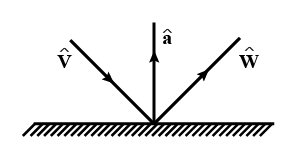
\includegraphics[width=\columnwidth]{20/img.png}
 \caption{}
 \label{fig:img}
 \end{figure}

\end{enumerate}
  
\section*{F  :  Match The Following}
 
 DIRECTIONS (Q. 1-6): Each question contains statements given in two columns, which have to be matched. The statements in Column-I are labelled 1, 2, 3 and 4. while the statements in Columa-II are labelled as a,b,c, d and e. Any given statement in Column-I can have correct matching with ONE OR MORE statement(s) in Column-II. The appropriate bubbles corresponding to the answer to these questions have to be darkened as illustrated in the following example:
If the correct matches are 1-a. s and e: 2-b and c: 3-1 and 2: and 4-d 

\begin{enumerate}
\item Match the following.(2006)\\

\begin{multicols}{2}
column-I \\
column-II

\end{multicols}

\begin{matchtabular}

Two rays $x+y=\mid a\mid$ and $ax-y=1$ intersects eachother in the first quadrant in the interval $a \in (a_0,\infty)$, the value of $a_0$ is &  2 \\
Point $(\alpha,\beta,\gamma)$ lies on the plane $x+y+z=2$.
Let $\vec{a}=\alpha\hat{i}+\beta\hat{j}+\gamma\hat{k}$,$\hat{k} \times \brak{\hat{k}\times\vec{a}}=0$, then $\gamma=$ & $\frac{4}{3}$\\
$\Bigg |\int_{0}^{1}\brak{1-y^2}dy|+\Bigg | \int_{1}^{0}\brak{y^2-1}dy|$ & $\Bigg |\int_{0}^{1}\sqrt{1-x}dx|+\Bigg | \int_{-1}^{0}\sqrt{1-x}dx|$\\
If $\sin A \sin B \sin C+ \cos A\cos B=1$,then the value of $\sin C=$ & 1\\

\end{matchtabular}

\item Consider the following linear equations\\
$ax+by+cz=0$;$bx+cy+az=0$;$cx+ay+bz=0$\\
Match the coditions/expressions in Column I with statements in Column II.(2007)
\begin{multicols}{2}
column-I \\
column-II
\end{multicols}

\begin{matchtabular}
$a+b+c\neq 0$and$a^2+b^2+c^2=ab+bc+ca$ & the equation represent planes meeting only at a single point\\
$a+b+c=0$and$a^2+b^2+c^2 \neq ab+bc+ca$ & the equation represent the line $x=y=z$\\
$a+b+c\neq 0$and$a^2+b^2+c^2 \neq ab+bc+ca$ & the equation representidentical planes.\\
$a+b+c=0$and$a^2+b^2+c^2=ab+bc+ca$ & the equation represent the whole of the three dimensional space.

\end{matchtabular} 

\item Match the statements/expressions given in Column I with the values given in Column II.(2009)

\begin{multicols}{2}
column-I \\
column-II

\end{multicols}

\begin{matchtabular}

Root(s)of the equation $2\sin^2\theta +\sin^22\theta =2$ & $\frac{\pi}{6}$\\
Points of discontinuity of the function $f(x)=\sbrak{\frac{6x}{\pi}\cos\frac{3x}{\pi}}$,f where [y] denotes the largest integer less than or equal to y & $\frac{\pi}{4}$\\
Volume of the parallelopiped with it's edges represented by the vectors $\hat{i}+\hat{j},\hat{i}+2\hat{j}$ and $\hat{i}+\hat{j}+\pi \hat{k}$ & $\frac{\pi}{2}$\\
Angle beteen vector $\vec{a} and \vec{b}$ where $\vec{a}, \vec{b} and \vec{c}$ are unit vectors satisfying $\vec{a}+\vec{b}+\sqrt{3}\vec{c}=0$ & $\pi$

\end{matchtabular}

\item Match the statements/expressions given in Column I with the values given in Column II.(2009)

\begin{multicols}{2}
column-I \\
column-II

\end{multicols}

\begin{matchtabular} 

The number of solution of the given $x e^{\sin x} -\cos x=0$ in the interval $\sbrak{0,\frac{\pi}{2}}$ & 1\\
Value(s) of k for which the planes $kx+4y+z=0,4x+ky+2z=0$ and $2x+2y+z=0$ intersects in a straight line.& 2\\
Value(s) of k for which $\mid x-1 \mid +\mid x-2\mid +\mid x+1\mid+\mid x+2\mid=4k$ has integer solution(s) & 4\\
If $y'=y+1$ and $y(0)=1$,then value(s) of y(1 and 2) & 5\\

\end{matchtabular}

\item Match the statements/expressions given in Column I with the values given in Column II.(2009)

\begin{multicols}{2}
column-I \\
column-II

\end{multicols}

\begin{matchtabular} 

A line from the origin meets the lines $\frac{x-2}{1}=\frac{y-1}{-2}=\frac{z+1}{1}$ and $\frac{x-\frac{8}{3}}{2}=\frac{y+3}{-1}=\frac{z-1}{1}$ at P and Q respectively.If length PQ=d,thej $d^2$ is & -4\\
The value of x satisfying $\tan^{-1}\brak{x+3}-\tan^{-1}\brak{x-3}=\sin^{-1}\sbrak{\frac{3}{5}}$ are & 0\\
Non-zero vectors $\vec{a}, \vec{b}$ and $\vec{c}$ satisfy $\vec{a}\cdot\vec{b}=0$.$\brak{\vec{b}-\vec{a}}\cdot \brak{\vec{b}+\vec{c}}=0$ and $2\mid \vec{b}+\vec{c}\mid=\mid \vec{b}-\vec{a}\mid$. If $\vec{a}=\mu\vec{b}+4\vec{c}$,then the possible values of $\mu$ are & 4\\
Let f be the function on $[-\pi,\pi]$ given by $f(0)=9$ and $f(x)=\frac{\sin\frac{9x}{2}}{\sin\frac{x}{2}} $ for $x\neq 0$. The value of $\frac{2}{\pi}\int_{-\pi}^{\pi}f(x)dx$ is & 5\\    & 6\\


\end{matchtabular}


\item Match the statements/expressions given in Column I with the values given in Column II.(2010)

\begin{multicols}{2}
column-I \\
column-II

\end{multicols}

\begin{matchtabular} 

If $\vec{a}=\hat{j}+\sqrt{3}\hat{k},\vec{b}=-\hat{j}+\sqrt{3}\hat{k}$ and $\vec{c}=\sqrt[2]{3}\hat{k}$ form a triangle, then the internal angle of the triangle between $\vec{a}$ and $\vec{b}$ is & $\frac{\pi}{6}$\\
If $\int_{a}^{b}\brak{f(x)-3x}dx=a^2-b^2$, then the value of $f\sbrak{\frac{\pi}{6}}$ is  & $\frac{2\pi}{3}$\\
The value of $\frac{\pi^2}{ln^3} \int_{\frac{5}{6}}^{\frac{7}{6}}\sec(\pi  x)dx$ is & $\frac{\pi}{3}$\\
The maximum vaalue of $\Bigg | arg\sbrak{\frac{1}{1-z}}\Bigg |  for \mid z \mid =1,z\neq 1$ is given by & $\pi$\\ & $\frac{\pi}{2}$\\


\end{matchtabular}

DIRECTIONS (Q. 7-9): Each question has matching lists have chances (p),(q),(r) and (s) out of which ONLY ONE  is correct.

\item Match List I with  List II and select the answer using the code given below the list

\begin{multicols}{2}
List-I \\
List-II

\end{multicols}

\begin{matchtabular} 
Volume of parallelopiped determined by vectors $\vec{a},\vec{b}$ and $\vec{c}$ is 2.Then the volume of parallelopiped determined by vectors $2\brak{\vec{a}\times\vec{b}},3\brak{\vec{b}\times\vec{c}}$ and $2\brak{\vec{c}\times\vec{a}}$ is  & 100\\
Volume of parallelopiped determined by vectors $\vec{a},\vec{b}$ and $\vec{c}$ is 5.Then the volume of parallelopiped determined by vectors $3\brak{\vec{a}+\vec{b}},3\brak{\vec{b}+\vec{c}}$ and $2\brak{\vec{c}+\vec{a}}$ is  & 30\\
Area of triangle with adjcent sides determined by the vectors  $\vec{a}$ and $\vec{b}$ is 20. Then the area of triangle with adjcent sides determined by the vectors $\brak{3\vec{a}+2\vec{b}}$ and $\brak{\vec{a}-\vec{b}}$ is & 24\\
Area of parallelogram with adjcent sides determined by the vectors  $\vec{a}$ and $\vec{b}$ is 30. Then the area of parallelogram with adjcent sides determined by the vectors $\brak{\vec{a}+\vec{b}}$ and $\vec{a}$ is & 60\\

\end{matchtabular}

Codes:\\
 \begin{tabular}{c c c c c}
             & 1 & 2 & 3 & 4 \\
         (p) & d & b & c & a \\
         (q) & b & c & a & d \\
         (r) & c & d & a & b \\
         (s) & a & d & c & b \\
        \end{tabular}
 
 
\item Consider the lines $L_1: \frac{x-1}{2}=\frac{y}{-1}=\frac{z+3}{1}$,$L_2:\frac{x-4}{1}=\frac{y+3}{1}=\frac{z+3}{2}$ and the planes $P_1: 7xy+2z=3$, $P_2=3x+5y-6z=4$.Let $ax+by+cz=d$ be the equation of the plane pasing through the point of intersection of lines $L_1$ and $L_2$ and erpedicular to plane $P_1$ and $P_2$.\\ (2013)


Match List I with  List II and select the answer using the code given below the list

 
\begin{multicols}{2}
List-I \\
List-II

\end{multicols}

\begin{matchtabular} 
a = & 13\\
b = & -3\\
c = &  1\\
d = & -2\\
 
\end{matchtabular}
 
Codes:\\
\begin{tabular}{c c c c c}
             & 1 & 2 & 3 & 4 \\
         (p) & c & b & d & a \\
         (q) & a & c & d & b \\
         (r) & c & b & a & d \\
         (s) & b & d & a & c \\
 \end{tabular}
\item Match List I with  List II and select the answer using the code given below the list  (2014)
 
\begin{multicols}{2}
List-I  \\
List-II  \\
7
\end{multicols}

\begin{matchtabular} 

Let $y(x)=\cos\brak{2\cos^{-1}x},x\in \sbrak{-1,1},x\neq \pm \frac{\sqrt{3}}{2}$. Then $\frac{1}{y(x)} \bigg\{ \brak{x^2-1}\frac{d^{2}y(x)}{dx^2}+\frac{dy(x)}{dx}\bigg\}$ equals & 1\\
Let $A_1,A_2....A_n(n>2)$ be the vertices of a regular polygon of n sides with it's center at the origin. Let $\vec{a_k}$ be the position vector of the points $A_k,k=1,2,...,n$. If $ \Bigg | \sum_{k=1}^{n-1}\sbrak{\vec{a_k}\times \vec{a_k+1}}\Bigg |$=$\Bigg | \sum_{k=1}^{n-1}\sbrak{\vec{a_k}\cdot \vec{a_k+1}}\Bigg | $,then the minimum value of n is & 2\\
If the normal from the point $p(h,1)$ on the ellipse $\frac{x^2}{6}+\frac{y^2}{3}=1$ is perpendicular to the line $x+y=8$, then the value of h & 8\\
Number of positive solution satisfying the equation $\tan^-1\frac{1}{2x+1}+\tan^-1\frac{1}{4x+1}=\tan^-1\frac{2}{x^2}$ is & 9\\

\end{matchtabular}
Codes:\\
\begin{tabular}{c c c c c}
             & 1 & 2 & 3 & 4 \\
         (p) & d & c & b & a \\
         (q) & b & d & c & a \\
         (r) & d & c & a & b \\
         (s) & b & d & a & c \\
 \end{tabular}

DIRECTIONS (Q.10-11): Refer to directions (1-6).
\item Match the following: (2015)

\begin{multicols}{2}
column-I \\
column-II

\end{multicols}

\begin{matchtabular} 
In $R^2$, if the magnitude of the projection vector of the vector $\alpha \hat{i}+\beta \hat{j}$ on $\sqrt{3}\hat{i}+\hat{j}$ is $\sqrt{3}$ and if $\alpha =2+\sqrt{3}\beta$, the possible value of $\mid \alpha \mid$ is/are & 1\\
Let a and b be real numbers such that the function $f(x)= \bigg \{$
 \begin{tabular}{ c c }
 $-3ax^{2}-2$, & $x < 1$ \\ 
 $ bx+a^2$, & $x\ge 1 $ \\
 \end{tabular} 
is differentiable for all $x \in R$ Then possible value of a is (are) & 2 \\
Let $\mu\neq 1$ be a complex cube root of unity. If $\brak{3-3\mu+2\mu^2}^{4n+3}+\brak{2+3\mu-3\mu^2}^{4n+3}+\brak{-3+2\mu+3\mu^2}^{4n+3}=0$ then possible value(s) of n is (are) & 3\\
Let the harmonic mean of two possitive real numbers a and b be 4. If q is a positive real number such that a,5,q,b is an arithmetic progression, then the value(s) of $\mid q-a \mid$ is (are) & 4 \\ & 5\\


\end{matchtabular}

\item match the following:  (2015)

\begin{multicols}{2}
column-I \\
column-II

\end{multicols}

\begin{matchtabular} 
In a triangle $\triangle XYZ$, let a,b and c be the length of the sides opposite to the angles X,Y and Z respectively. If $2\brak{a^2-b^2}=1$ and  $\lambda=\frac{\sin X-Y}{\sin Z}$, then possible values of n for which $\cos (n\pi\lambda)=0$ is(are) & 1\\
In a triange $\triangle XYZ$, let a,b and c be length of the sides opposite to the angles X,Y and Z respectively. If $1+\cos 2X-2\cos 2Y=2\sin X \sin Y$, then possible value(s) of $\frac{a}{b}$ is (are) &2\\
In $R^2$, let $\sqrt{3}\hat{i}+\hat{j},\hat{i}+\sqrt{3}\hat{j}$ and $\beta\hat{i}+\brak[1-\beta\hat{j}$ be position vectors of X,Y and Z with respect to origin O,respectively . If the distance of Z from the bisector of the acute angle of $\vec{OX}$ with $\vec{OY}$is $\frac{3}{\sqrt{2}}$, then possible value(s) of $\mid \beta \mid $ is (are) & 3\\
Suppose that $F(\alpha)$ denotes the area of the region bounded by $x=0,x=2,y^{2}=4x$ and $y=\mid \alpha x-1 \mid+\mid \alpha x-2 \mid+\alpha x $  where $\alpha \in {0,1}$ . Then the value(s) of $F(\alpha)+\frac{8}{3}\sqrt{2}$, when $\alpha=0$ and $\alpha=1$ is(are) & 5\\ & 6\\

\end{matchtabular}
\end{enumerate}
\section*{F  :  Comprehension Based Questions}

Consider the lines $L_1:\frac{x+1}{3}=\frac{y+2}{1}=\frac{z+1}{2}$ $L_2:\frac{x-2}{1}=\frac{y+2}{2}=\frac{z-3}{3}$

\begin{enumerate}
\item The unit vector perpendicular to both $L_1$ and $L_2$ is  (2008)
\begin{enumerate}
\item $\frac{-\hat{i}+7\hat{j}+7\hat{k}}{\sqrt{99}}$
\item $\frac{-\hat{i}-7\hat{j}+5\hat{k}}{\sqrt[5]{3}}$
\item $\frac{-\hat{i}+7\hat{j}+5\hat{k}}{\sqrt[5]{3}}$
\item $\frac{7\hat{i}-7\hat{j}-\hat{k}}{\sqrt{99}}$
\end{enumerate}
\item The shortest distance between $L_1$ and $L_2$ is  (2008)
\begin{enumerate}
\item $\frac{17}{\sqrt{3}}$ 
\item 0
\item $\frac{41}{\sqrt[5]{3}}$ 
\item $\frac{17}{\sqrt[5]{3}}$ 
\end{enumerate}
\item The distance of the point(1,1,1) from the plane passing through the point(-1,-2,-1) wwhose normal is perpendicular to both the lines $L_1$ and $L_2$ is  (2008)
\begin{enumerate}
\item  $\frac{2}{\sqrt{75}}$
\item  $\frac{7}{\sqrt{75}}$  
\item  $\frac{13}{\sqrt{75}}$ 
\item  $\frac{22}{\sqrt{75}}$ 
\end{enumerate}
\end{enumerate}

\section*{H   :  Assertion And Reason Type Questions}

\begin{enumerate}
\item Consider the plane $3x-6y-2z=15$ and $2x+y-2z=5$.
 STATEMENT-1: The parametric equations of the line of intersection of the given planes are $x=3+14t$,$y=1+2t$ and $z=15t$ because
 STATEMENT-2: The vector $14i + 2j+15k$ is parallel to the line of intersection of given planes. (2007)
\begin{enumerate}
\item Statement-1 is True, Statement-2 is True; Statement-2 is a correct explanation for Statement-1 
\item Statement-1 is True, Statement-2 is True; Statement-2 is NOT a correct explanation for Statement-1
\item Statement-1 is True, Statement-2 is False
\item Statement-1 is False, Statement-2 is True.
\end{enumerate}
\item Let the vectors $\vec{PO}, \vec{OR}, \vec{RS}, \vec{ST}, \vec{TU}$ and $\vec{JP}$ represent the sides ofa regular hexagon.
STATEMENT-1: $\vec{PQ}\times\brak{\vec{RS}+\vec{ST}}\neq \vec{0}$.because
 STATEMENT-2: $\vec{PQ}\times\vec{RS}=\vec{0}$ and $\vec{PQ}\times \vec{ST}\neq \vec{0}$
 (2007)
 \begin{enumerate}
\item Statement-1 is True, statement-2 is True; Statement-2 is a correct explanation for Statement-1.
\item Statement-1 is True, Statement-2 is True, Statement2 is NOT a correct explanation for Statement-1
\item  statement-1 is True, Statement-2 is False
\item  Statement-1 is False, Statement-2 is True.
\end{enumerate}
\item Consider three planes $P_1:x-y+z=1$ $x+y-z=1$ $x-3y+3z=2$ let $L_1,L_2,L_3$ be the lines of intersection of the planes $P_2$ and $P_3$,$P_3$ and $P_1$ , $P_2$ and $P_1$ respectively.\\
STATEMENT-1Z: At least two of the lines $L_1, L_2$ and $L_3$ are non-parallel and\\
STATEMENT-2: The three planes dose not have a common point. (2008)
\begin{enumerate}
\item STATEMENT -1 is True, STATEMENT -2 is True; STATEMENT - 2 is a correct explanation for STATEMENT- 1
\item STATEMENT - 1 is True, STATEMENT - 2 is True; STATEMENT - 2 is NOT a correct explanation for STATEMENT- 1
\item STATEMENT-1 is True, STATEMENT -2 is False
\item STATEMENT - 1 is False, STATEMENT-2 is True
\end{enumerate}

\end{enumerate}

\section*{I    : Integer Value Correct Type }

\begin{enumerate}
\item If $\vec{a}$ and $\vec{b}$ are vectors in space given by $\vec{a}=\frac{\hat{i}-2\hat{j}}{\sqrt{5}}$ and $\vec{b}=\frac{2\hat{i}+\hat{j}+3\hat{k}}{\sqrt{14}}$,then find the value of $\brak{2\vec{a}+2\vec{b}}\cdot\sbrak{\brak{\vec{a}\times\vec{b}}\times\brak{\vec{a}-2\vec{b}}}$.(2010)
\item If the distance between the plane $Ax-2y +z=d$ and the plane containing the lines 
$\frac{x-1}{2}=\frac{y-2}{3}=\frac{z-3}{4}$ and $\frac{x-2}{3}=\frac{y-3}{4}=\frac{z-4}{5}$ is $\sqrt{6}$ then find $\mid d \mid$.(2010)
\item Let $\vec{a}=-\hat{i}-\hat{k},\vec{b}=-\hat{i}+\hat{j}$ and $\vec{c}=\hat{i}+2\hat{j}+3\hat{k}$ be three given vectors. If $\vec{r}$ is a vector such that $\vec{r} \times\vec{b}=\vec{c}\times\vec{b}$ and $\vec{r}\cdot\vec{a}=0$, then the value of $\vec{r}\cdot\vec{b}$ is (2011)
\item If $\vec{a},\vec{b}$ and $\vec{c}$ are unit vectors satisfying $\mid \vec{a}-vec{b}\mid^{2}+\mid \vec{b}-vec{c}\mid^{2}+\mid +\mid \vec{c}-vec{a}\mid^{2}+\mid=9$, then $2\vec{a}+5\vec{b}+5\vec{c}$ is (2012)
\item Consider the set of eight vectors $V={a\hat{i}+b\hat{j}+c\hat{k};a,b,c\in {-1,1} }$. Three non-coplanar vectors can be chosen from V in $2^p$ ways. Then p is (2013)
\item A pack contains n cards numbered from 1 to n. Two consecutive numbered cards are removed from the pack and the sum of the numbers on the remaining cards is 1224. If the
smaller of the numbers on the removed cards is k, then $K-20=$ is (2013)
\item Let $\vec{a},\vec{b}$ and $\vec{c}$ be three non-coplanar unit vectors such that the angle between every pair of them is $\frac{\pi}{3}$. If $\vec{a}\times\vec{b}+\vec{b}\times\vec{c}=\overrightarrow{pa}+\overrightarrow{qb}+\overrightarrow{rc}$, where p,q and r are scalars then the value of $\frac{p^{2}+2q^{2}+r^{2}}{q^2}$is (2014)
\item  Suppose that $\vec{p},\vec{q}$ and $\vec{r}$ are three non-coplanar unit vectors i $R^3$.Let the components of vector $\vec{s}$ along $\vec{p},\vec{q}$ and $\vec{r}$ be 4,3 and 5 respectively. If the components of this vector $\vec{s}$ along $\brak{-\vec{p}+\vec{q}+\vec{r}}$,$\brak{\vec{p}-\vec{q}+\vec{r}}$ and $\brak{-\vec{p}-\vec{q}+\vec{r}}$ are x,y and z respectively, then the value of $2x+y+z$ is (2015)
\item Let $\vec{a}$ and $\vec{b}$ be two unit vectors such that $\vec{a}\cdot\vec{b}=0$. For some $x,y\in R$, let $\vec{c}=x\vec{a}+y\vec{b}+\brak{\vec{a}\times\vec{b}}$. If $\vec{c}=2$ and the vector $\vec{c}$ is inclined at the same angle $\alpha$ to both $\vec{a}$ and $\vec{b}$ then the value of $8\cos^2\alpha$ is .......(2018)
\item Let P be a point in  the first octant, whose image Qin the plane $x+y=3$(that is,the line segment PQ is perpendicular to the plane $x+y=3$ end the mid-point of PQ lies in the planr $x=y=3$)lies on the z-axis.Let the distance of P from the x-axis be 5. If R is the image of P in the xy-plane,then the length of PR is.....(2018)
\item Consider the cube in the first octant with sides OP,OQ and OR of length 1, along the a-axis and z-axis,respectively,where $O(0,0,0)$ is the origin. Let $S\sbrak{\frac{1}{2},\frac{1}{2},\frac{1}{2}}$ be the center of the cube and T be the vertex of the cube opposite to the origin O such that S lies on the diagonal OT. If $\vec{p}=\overrightarrow{SP},\vec{q}=\overrightarrow{SQ},\vec{r}=\overrightarrow{SR}$ and $\vec{t}=\overrightarrow{ST}$, then the value of $\mid \brak{\vec{p}\times\vec{q}}\times\brak{\vec{r}\times\vec{t}}\mid$ is ......(2018)
\item Three lines are given by $\vec{r}=\lambda \hat{i},\lambda \in R$;$\vec{r}=\mu \brak{\hat{i}+\hat{j}},\mu \in R$ and $\vec{r}=\gamma\brak{\hat{i}+\hat{j}+\hat{k},\gamma\in R}$. Let the lines cuts the plane $x+y+z=1$ at the points A,B and C respectively. If the area of the triangle ABC is $\triangle$ then the value of $\brak{6\triangle^2}$ equals ......(2019)
\item Let $\vec{a}=2\hat{i}+\hat{j}-\hat{k}$ and $\vec{b}=\hat{i}+2\hat{j}-\hat{k}$ be two vectors. Consider a vector $\vec{c}=\alpha\vec{a}+\beta\vec{b},\alpha,\beta \in R$. If the projection of $\vec{c}$ on the vector $\brak{\vec{a}-\vec{b}}$ is $\sqrt[3]{2}$, then the minimum vakue of $\sbrak{\vec{c}-\brak{\vec{a}\times\vec{b}}}\vec{c}$ equals.........(2019)

\end{enumerate} 
\section*{Section-B    [JEE Advanced/IIT-JEE]}
\section*{A    :  Fill in the Blanks}

\begin{enumerate}
\item A plane which passes through the point (3, 2, 0) and the line $\frac{x-4}{1}=\frac{y-7}{5}=\frac{z-4}{4}$ is (2002)
\begin{enumerate}
\item $x-y+z=1$
\item $x+y+z=5$
\item $x+2y-z=1$
\item $2x-y+z=5$
\end{enumerate}
\item If  $\mid \vec{a} \mid =4$,$\mid \vec{b}  \mid =2$ and the angle between $\vec{a}$ and $\vec{b}$ is $\frac{\pi}{6}$ then $\brak{\vec{a}\times\vec{b}}^2$ is equal to (2002)
\begin{enumerate}
\item  48
\item 16
\item $\vec{a}$
\item None of these
\end{enumerate}
\item If $\vec{a},\vec{b},\vec{c}$ are vectors such that 
$
\begin{bmatrix}
\vec{a} & \vec{b} & \vec{c} =4
\end{bmatrix}$
then 
$
\begin{bmatrix}
 \vec{a}\times\vec{b} &\vec{b}\times \vec{c} & \vec{c}\times\vec{a}
\end{bmatrix}$=
\begin{enumerate}
\item 16
\item 64 
\item 4 
\item 8
\end{enumerate}
\item If $\vec{a},\vec{b},\vec{c}$ are vectors show that $\vec{a}+\vec{b}+\vec{c}=0$ and 
 $\mid \vec{a} \mid=7,\mid \vec{b} \mid=5,\mid \vec{c} \mid=3 $ then angle between vector $\vec{b}$ and $\vec{c}$ is (2002)
\begin{enumerate}
\item  $60^\circ $
\item  $30^\circ $
\item  $45^\circ $
\item  $90^\circ $
\end{enumerate}
\item If $\mid \vec{a} \mid=5,\mid \vec{b} \mid=4,\mid \vec{c} \mid=3 $ thus what will be the value of $\mid \vec{a} \cdot \vec{b}+\vec{b}\cdot\vec{c}+\vec{c}\cdot\vec{a} \mid$, given that $\vec{a}+\vec{b}+\vec{c}=0$
\begin{enumerate}
\item 25
\item 50
\item -25
\item -50
\end{enumerate}
\item If the vector $\vec{c},\vec{a}=x\hat{i}+y\hat{j}+z\hat{k}$,$\vec{b}=\hat{j}$ are such that $\vec{a},\vec{b},\vec{c}$ form a right handed system then $\vec{c}$ is
\begin{enumerate}
\item $z\hat{i}-x\hat{k}$
\item $\vec{0}$
\item $y\hat{j}$
\item $-z\hat{i}+x\hat{k}$
\end{enumerate}
\item $\vec{a}=3\hat{i}-5\hat{j}$ and $\vec{b}=6\hat{i}+3\hat{j}$ are two vectors and $\vec{c}$ is a vector such that $\vec{c}=\vec{a}\times\vec{b}$ then $\mid \vec{a}\mid:\mid \vec{b} \mid:\mid \vec{c}\mid$(2002)
\begin{enumerate}
\item $\sqrt{34}:\sqrt{45}:\sqrt{39}$
\item $\sqrt{34}:\sqrt{45}:39$
\item 34:39:45
\item 39:35:34
\end{enumerate}
\item IF $\vec{a}\times\vec{b}=\vec{b}\times\vec{c}=\vec{c}\times\vec{a}$ then $\vec{a}+\vec{b}+\vec{c}=$
\begin{enumerate}
\item abc
\item -1
\item 0
\item 2
\end{enumerate}
\item The d.r. of normal to the plane through $(1, 0, 0), (0, 1,0)$ which makes an angle$\frac{\pi}{4}$ with plane $x+y=3$ are (2002)
\begin{enumerate}
\item  1,$\sqrt{2}$,1
\item  1,1,$\sqrt{2}$
\item  1,1,2
\item  $\sqrt{2}$,1,1
\end{enumerate}
\item Let $\vec{u}=\hat{i}+\hat{j}$,$\vec{v}=\hat{i}-\hat{j}$ and $\vec{w}=\hat{i}+2\hat{j}+3\hat{k}$. If $\hat{n}$ is a unit vector such that $\vec{u}\cdot\hat{n}=0$ and  $\vec{v}\cdot\hat{n}=0$ then $\mid \vec{w}\cdot\hat{n}\mid$ is equals to (2003)
\begin{enumerate}
\item 3
\item 0
\item 1
\item 2
\end{enumerate}
\item  A particle acted on by constant forces $4\hat{i}+\hat{j}-3\hat{k}$ and $3\hat{i}+\hat{j}-\hat{k}$ is displaced from the point $\hat{i}+2\hat{j}-3\hat{k}$to the point $5\hat{i}+4\hat{j}+\hat{k}$. The total work done by the force is (2003)
\begin{enumerate}
\item 50 units
\item 20 units
\item 30 units
\item 40 units
\end{enumerate}
\item The vector $\overrightarrow{AB}=3\hat{i}+4\hat{k} \& \overrightarrow{AC}= 5\hat{i}-2\hat{j}+4\hat{k}$ are the sides of triangle ABC. The length of the median through A is (2003)
\begin{enumerate}
\item $\sqrt{288}$
\item $\sqrt{18}$
\item $\sqrt{72}$
\item $\sqrt{33}$
\end{enumerate}
\item The shortest distance from the plane $12x+4y+3z=327$ to the sphere $x^2+y^2+z^2+4x-2y-6z=155$ is
\begin{enumerate}
\item 39
\item 26 
\item $11\frac{4}{13}$
\item 13
\end{enumerate}
\item The two lines $x=ay+b$, $z=cy+d$ and $x=a^{}y+b^{}$, $z=c^{}y+a^{}$ will be perpendicular, if and only if (2003)
\begin{enumerate}
\item $aa^{'}+cc^{'}+1=0$
\item $aa^{'}+bb^{'}+cc^{'}+1=0$
\item $aa^{'}+bb^{'}+cc^{'}=0$
\item $\brak{a+a^{'}}\brak{b+b^{'}}+\brak{c+c^{'}}$
\end{enumerate}
\item The lines $\frac{x-2}{1}=\frac{y-3}{1}=\frac{z-4}{-k}$ and $\frac{x-1}{k}=\frac{y-4}{1}=\frac{z-5}{1}$ are coplanar if (2003)
\begin{enumerate}
\item k=3 or -2
\item k= 0 or -1
\item k= 1 or -1
\item k=0 or -3
\end{enumerate}
\item If $\vec{a},\vec{b} ,\vec{c}$ are three vectors such that $\vec{a}+\vec{b}+\vec{c}=0$,$\mid \vec{a} \mid=1$,$\mid \vec{b} \mid=2$ and $\mid \vec{c} \mid=3$ then $\vec{a}\cdot\vec{b}+\vec{b}\cdot\vec{c}+\vec{c}\cdot\vec{a}$ is equal to (2003)
\begin{enumerate}
\item 1
\item 0
\item -7 
\item 7
\end{enumerate}
\item The radius of the circle in which the sphere $x^2+y^2+z^2+2x-2y-4z-19=0$ is cut by the plane $x+2y+2z+7=0$ (2003)
\begin{enumerate}
\item 4
\item 1
\item 2 
\item 3
\end{enumerate}
\item A tetrahedron has vertices at$O(0,0,0),A(1,2,1)B(2,1,3)$ and $C(-1,1,2)$. Then the angle between the faces OAB and ABC will be (2003)
\begin{enumerate}
\item $90^\circ$ 
\item $\cos^-{1}\frac{19}{35}$ 
\item $\cos^-{1}\frac{17}{31}$ 
\item $30^\circ$ 
\end{enumerate}
\item If $\begin{vmatrix}
 a & a^2  & 1+a^3\\
 b   & b^2 & 1+b^3\\
 c    & c^2 & 1+c^3
\end{vmatrix}=0$ \\ and vectors $(1,a,a^2)$,$(1,b,b^2)$ and $(1,c,c^2)$ are non-coplanar, then the product abc equals (2003)
\begin{enumerate}
\item 0
\item 2
\item -1
\item 1
\end{enumerate}
\item  Consider points A,,B,C and D  with position vectors $7\hat{i}-4\hat{j}+7\hat{k}$,$\hat{i}-6\hat{j}+10\hat{k}$,$-\hat{i}-3\hat{j}+\hat{k}$ and $5\hat{i}-\hat{j}+\hat{k}$ respectively. Then ABCD is a (2003)
\begin{enumerate}
\item parllelogram but not a rhombus
\item square
\item rhombus
\item rectangle
\end{enumerate}
\item If $\vec{u},\vec{v}$ and $\vec{w}$ are three non-planar vectors then $\brak{\vec{u}+\vec{v}-\vec{w}}\cdot\brak{\vec{u}-\vec{w}}\times\brak{\vec{v}-\vec{w}}$ equals (2003)
\begin{enumerate}
\item $3\vec{u}\cdot\vec{v}\times\vec{w}$
\item 0
\item $\vec{u}\cdot\vec{v}\times\vec{w}$
\item $3\vec{u}\cdot\vec{w}\times\vec{v}$
\end{enumerate}
\item Two system of rectangular axes have the same origin. If a plane cuts them at distances a,b,c and $a^{'},b^{'},c^{'}$ from the origin then (2003)
\begin{enumerate}
\item $\frac{1}{a^2}+\frac{1}{b^2}+\frac{1}{c^2}-\frac{1}{a'^2}-\frac{1}{b'^2}-\frac{1}{c'^2}=0$
\item $\frac{1}{a^2}+\frac{1}{b^2}+\frac{1}{c^2}+\frac{1}{a'^2}+\frac{1}{b'^2}+\frac{1}{c'^2}=0$
\item $\frac{1}{a^2}+\frac{1}{b^2}-\frac{1}{c^2}+\frac{1}{a'^2}+\frac{1}{b'^2}-\frac{1}{c'^2}=0$
\item $\frac{1}{a^2}-\frac{1}{b^2}-\frac{1}{c^2}+\frac{1}{a'^2}-\frac{1}{b'^2}-\frac{1}{c'^2}=0$
\end{enumerate}
\item Distance between two parallel planes $2x+y+2z=8$ and $4x+2y+4z+5=0$ is (2004)
\begin{enumerate}
\item $\frac{5}{2}$
\item $\frac{9}{2}$
\item $\frac{7}{2}$
\item $\frac{3}{2}$
\end{enumerate}
\item A line with dircction cosines proportional to 2, 1,2 meets each of the lines each of the lines $x=y+a=z$ and $x+a=2y=2z$. The coordinates of each of the points of intersection is given by (2004)
\begin{enumerate}
\item $(2a,3a,3a),(2a,a,a)$
\item $(3a,2a,2a),(a,a,a)$
\item $(3a,2a,3a),(a,a,2a)$
\item $(3a,3a,3a),(a,a,a)$
\end{enumerate}
\item If the straight lines $x=1+s,y=-3-\lambda s,z=1+\lambda s$ and $x=\frac{t}{2},y=1+t,z=2-t$ with parameters s and t respectively, are co-planar then $\lambda$ is (2004)
\begin{enumerate}
\item 0
\item -1
\item $-\frac{1}{2}$
\item -2
\end{enumerate}
\item The intersection of the spheres $x^2+y^2+z^2+7x-2y-z=13$ and $x^2+y^2+z^2-3x+3y+4z=8$ is the same as the intersection of the sphere and the plane (2004)
\begin{enumerate}
\item $2x-y-z=1$
\item $x-2y-z=1$
\item $x-y-2z=1$
\item $x-y-z=1$
\end{enumerate}
\item Let $\vec{a},\vec{b}$ and $\vec{c}$ are three non-zero coplanar vectors such that no two of these are collinear. I the vector $\vec{a}+2\vec{b}$ is collinear with $\vec{c},\vec{b}+3\vec{c}$ is collinear with $\vec{a}$($\lambda$ being some non-zero scalar then $\vec{a}+2\vec{b}+6\vec{c}$ is equals (2004)
\begin{enumerate}
\item 0
\item $\lambda \vec{a}$
\item $\lambda \vec{b}$
\item $\lambda \vec{c}$
\end{enumerate} 
\item A particles is acted upon by constant force $4\hat{i}+\hat{j}-3\hat{k}$ and $3\hat{i}+\hat{j}-\hat{k}$ which displace it from a point $\hat{i}+2\hat{j}+3\hat{k}$ to the point $5\hat{i}+4\hat{j}+\hat{k}$.The work done in standard units by the forces is given by (2004)
\begin{enumerate}
\item 15
\item 30
\item 25 
\item 40
\end{enumerate} 
\item If $\vec{a},\vec{b},\vec{c}$ are non coplanar vectors and $\lambda$ is a real number then the vectors $\vec{a}+2\vec{b}+3\vec{c}$ $\lambda\vec{b}+4\vec{c}$ and $\brak{2\lambda-1}\vec{c}$ are non-coplanar for(2004) 
\begin{enumerate}
\item  No value for $\lambda$
\item  All expect one value for $\lambda$
\item  All expect two value for $\lambda$
\item  ALL values of $\lambda$
\end{enumerate}

\item Let $\vec{u},\vec{v},\vec{w}$ be such that $\mid \vec{u} \mid =1, \mid \vec{v}\mid =2$ and $\mid \vec{w} \mid =3$. If the projection $\vec{v}$ along $\vec{u}$ is equal to that of $\vec{w}$ along $\vec{u}$ and $\vec{v}$, $\vec{w}$ are perpendicular to each other then $\vec{u}-\vec{v}+\vec{w}$ equals(2004)
\begin{enumerate}
\item 14
\item $\sqrt{7}$
\item $\sqrt{14}$If the pane 
\item 2
\end{enumerate} 
\item Let $\vec{a},\vec{b},\vec{c}$ are non-zero vectors such that $\brak{\vec{a}\times\vec{b}}\times\vec{c}=\frac{1}{3} \mid \vec{b} \mid  \mid \vec{c} \mid$ $\vec{a}$. If $\theta$ is the acute angle between vectors $\vec{b}$ and $\vec{c}$ then $\sin \theta$ equals (2004)
\begin{enumerate}
\item $\frac{\sqrt[2]{2}}{3}$
\item $\frac{\sqrt{2}}{3}$
\item $\frac{2}{3}$
\item $\frac{1}{3}$
\end{enumerate}
\item If C is the mid-point of AB and P is any point outside AB, then (2005)
\begin{enumerate}
\item $\overrightarrow{PA}+\overrightarrow{PB}=2\overrightarrow{PC}$
\item $\overrightarrow{PA}+\overrightarrow{PB}=\overrightarrow{PC}$
\item $\overrightarrow{PA}+\overrightarrow{PB}+2\overrightarrow{PC}=0$
\item $\overrightarrow{PA}+\overrightarrow{PB}+\overrightarrow{PC}=0$
\end{enumerate}
\item If the angle $\theta$ between the lines $\frac{x+1}{2}=\frac{y-1}{2}=\frac{z-2}{2}$ and the plane $2x-y+\sqrt{\lambda}z+4=0$ is such that $\sin\theta=\frac{1}{3}$ then the value of $\lambda$ is (2005)
\begin{enumerate}
\item  $\frac{5}{3}$
\item $\frac{-3}{5}$
\item $\frac{3}{4}$
\item $\frac{-4}{3}$
\end{enumerate}
\item The angle between the lines $2x=3y=-z$ and $6x=-y=-4z$ is (2005)
\begin{enumerate}
\item $0^\circ$
\item $90^\circ$
\item $45^\circ$
\item $30^\circ$
\end{enumerate}
\item If the plane $2ax-3ay+4az+6=0$ passes through the mid-point of line joining the center of the spheres $x^2+y^2+z^2+6x-8y-2z=13$ and $x^2+y^2+z^2-10x+4y-2z=8$ then a equals (2005)
\begin{enumerate}
\item -1
\item 1
\item -2 
\item 2
\end{enumerate}
\item The distance between the line $\vec{r}=2\hat{i}-2\hat{j}+3\hat{k}+\lambda\brak{\hat{i}-\hat{j}+4\hat{k}}$ and the plane $\vec{r}\cdot\brak{\hat{i}+5\hat{j}+\hat{k}}=5$(2005)
\begin{enumerate}
\item $\frac{10}{9}$
\item $\frac{10}{\sqrt[3]{3}}$
\item $\frac{3}{10}$
\item $\frac{10}{3}$
\end{enumerate}
\item For any vector $\vec{a}$ , the value of $\brak{\vec{a}\times\hat{i}^2}+\brak{\vec{a}\times\hat{j}^2}+\brak{\vec{a}\times\hat{k}^2}$ is equal to (2005)
\begin{enumerate}
\item $3a^-2$
\item $a^-2$
\item $2a^-2$
\item $4a^-2$
\end{enumerate}
\item If non-zero numbers a, b, c are in H.P., then the straight line. $\frac{x}{a}+\frac{y}{b}+\frac{1}{c}=0$ always passes through a fixed point. That point is (2005)
\begin{enumerate}
\item $(-1,2)$
\item $(-1,-2)$
\item $(-1,-2)$
\item $(1,-\frac{1}{2})$
\end{enumerate}
\item Let a, b and c be distinct non-negative numbers. If the vectors $a\hat{i}+a\hat{j}+c\hat{k},\hat{i}+\hat{k},c\hat{i}+c\hat{j}+b\hat{k}$ lie in a plane, then c is (2005)
\begin{enumerate}
\item the Geometric Mean of a and b
\item the Arithmetic Mean of a and b
\item equal to zero
\item  the Harmonic Mean of a and b
\end{enumerate}
\item  If $\vec{a},\vec{b},\vec{c}$ are non-coplanar vectors and $\lambda$ is real number then 
$
\begin{bmatrix}
\lambda\brak{\vec{a}+\vec{b}} & \lambda^2\vec{b} & \lambda\vec{c} =
\end{bmatrix}$
$\begin{bmatrix}
\vec{a} & \vec{b}+\vec{c} & \vec{b} 

\end{bmatrix}
$ for (2005)
\begin{enumerate}
\item exactly one value of $\lambda$
\item no value $\lambda$
\item exactly three value of $\lambda$
\item exactly two value of $\lambda$
\end{enumerate}
\item Let $\vec{a}=\hat{i}-\hat{k},\vec{b}=x\hat{i}+\hat{j}+\brak{1-x}\hat{k}$ and $\vec{c}=y\hat{i}+x\hat{j}+\brak{1+x-y}\hat{k}$. Then $\sbrak{\vec{a},\vec{b},\vec{c}}$ depends on (2005)
\begin{enumerate}
\item only y
\item only x
\item both x and y
\item neither x nor y
\end{enumerate}
\item The plane $x+2y-z=4$ cuts the sphere $x^2+y^2+z^2-x+z-2=0$ in a circle of radius (2005)
\begin{enumerate}
\item 3 
\item 1
\item 2
\item $\sqrt{2}$
\end{enumerate}
\item If $\brak{\vec{a}\times\vec{b}}\times\vec{c}=\vec{a}\times\brak{\vec{b}\times\vec{c}}$ where $\vec{a},\vec{b},\vec{c}$ are any three vectors such that $\vec{a}\cdot \vec{b}\neq =$,$\vec{b}\cdot \vec{c}\neq =$ then $\vec{a}$ and $\vec{c}$ are (2005)
\begin{enumerate}
\item inclined at an angle of $\frac{\pi}{3}$ between them 
\item inclined at an angle of $\frac{\pi}{6}$ between them 
\item perpendicular
\item parallel
\end{enumerate}
\item The values of a, for which points A, B, C with position vectors  $2\hat{i}-\hat{j}+\hat{k},\hat{i}-3\hat{j}-5\hat{k}$ and $a\hat{i}-3\hat{j}+\hat{k}$ respectively are the vertices of a rightangled triangle with $c=\frac{\pi}{2}$ are (2005)
\begin{enumerate}
\item 2 and 1
\item -2 and -1
\item -2 and 1
\item 2 and -1
\end{enumerate}
\item  The two lines $x=ay+b$,$z=cy+d$ and $x=a'y+b',z=c'y+d'$ are perpendicular to each other if (2006)
\begin{enumerate}
\item $aa'+cc'=-1$
\item $aa'+cc'=1$
\item $\frac{a}{a'}+\frac{c}{c'}=-1$
\item $\frac{a}{a'}+\frac{c}{c'}=1$
\end{enumerate}
\item  The image of the point (-1, 3,4) in the plane $x-2y=1$ is (2006)
\begin{enumerate}
\item $\brak{\frac{-17}{3},\frac{-19}{3},4}$
\item (15,11,4)
\item $\brak{\frac{-17}{3},\frac{-19}{3},1}$
\item None of these
\end{enumerate}
\item If a line makes an angle of $\frac{\pi}{4}$ with the positive directions of each of x- axis and y- axis, then the angle that the line makes with the positive direction of the z-axis is (2006)
\begin{enumerate}
\item $\frac{\pi}{4}$
\item $\frac{\pi}{2}$
\item $\frac{\pi}{6}$
\item $\frac{\pi}{3}$
\end{enumerate}
\item If $\vec{u}$ and $\vec{v}$ are unit vectors and $\theta$ is the acute angle between them, then $2\vec{u}\times 3\vec{v}$ is a unit vector for (2007)
\begin{enumerate}
\item no value of $\theta$
\item exactly one value of $\theta$
\item exactly two value of $\theta$
\item more than two values of $\theta$
\end{enumerate}
\item If (2.3, 5) is one end of a diameter of the sphere $x^2+y^2+z^2-6x-12y-2z+20=0$ then the cooordinates of the other end of the diameter are  (2007)
\begin{enumerate}
\item (4,3,5)
\item (4,3,-3)
\item (4,9,-3)
\item (4,-3,3)
\end{enumerate}
\item Let $\vec{a}=\hat{i}+\hat{j}+\hat{k},\vec{b}=\hat{i}-\hat{j}+2\hat{k},\vec{c}=x\hat{i}+(x-2)\hat{j}-\hat{k}$. If the vectors lies in the plane of $\vec{a}$ and $\vec{b}$ , then x equals (2007)
\begin{enumerate}
\item -4
\item -2
\item 0
\item 1
\end{enumerate}
\item Let L be the line of intersection of the planes $2x+3y+z=1$ and $x+3y+2z=2$. If L makes an angle $\alpha$ with the positive x-axis, then $\cos \alpha$ equals (2007)
\begin{enumerate}
\item 1
\item $\frac{1}{\sqrt{2}}$
\item $\frac{1}{\sqrt{3}}$
\item $\frac{1}{2}$
\end{enumerate}
\item The vector $\vec{a}=\alpha\hat{i}+2\hat{j}+\beta\hat{k}$ lies in the plane of the vectors $\vec{b}=\hat{i}+\hat{j}$ and $\vec{c}=\hat{j}+\hat{k}$ and bisects the angle between $\vec{b}$ and $\vec{c}$. Then which one of the following gives possible
values of $\alpha$ and $\beta$ ? (2008) 
\begin{enumerate}
\item $\alpha=2,\beta=2$ 
\item $\alpha=1,\beta=2$ 
\item $\alpha=2,\beta=1$ 
\item $\alpha=1,\beta=1$ 
\end{enumerate}
\item The non-zero Vectors are $\vec{a},\vec{b}$ and $\vec{c}$ are related by $\vec{a}=8\vec{b}$ and $\vec{c}=-7\vec{b}$. Then the angle between $\vec{a}$ and $\vec{c}$ is (2008)
\begin{enumerate}
\item 0
\item $\frac{\pi}{4}$
\item $\frac{\pi}{2}$
\item $\pi$ 
\end{enumerate}
\item The line passing through the points (5, 1, a) and (3, b, 1) crosses the yz-plane at the point $\sbrak{0,\frac{17}{2},\frac{-13}{2}}$. Then (2008)
\begin{enumerate}
\item a=2,b=8
\item a=4,b=6
\item a=6,b=4
\item a=8,b=2
\end{enumerate}
\item If the straight lines $\frac{x-1}{k}=\frac{y-2}{2}=\frac{z-3}{3}$ and $\frac{x-2}{3}=\frac{y-3}{k}=\frac{z-1}{2}$ intersect at a point, then the integer k is equal to (2008)
\begin{enumerate}
\item -5
\item 5
\item 2
\item -2
\end{enumerate}
\item Let the line $\frac{x-2}{3}=\frac{y-2}{-5}=\frac{z+2}{2}$ lie in the plane $x+3y-\alpha z+\beta=0$ then $(\alpha,\beta)$ equals (2009)
\begin{enumerate}
\item (-6,7)
\item (5,-15)
\item (-5,5)
\item (6,-17)
\end{enumerate}
\item The projections of a vector on the three coordinate axis are 6,-3, 2 respectively. The direction cosines of the vector are:(2009)
\begin{enumerate}
\item $\frac{6}{5},\frac{-3}{5},\frac{2}{5}$ 
\item $\frac{6}{7},\frac{-3}{7},\frac{2}{7}$ 
\item $\frac{-6}{7},\frac{-3}{7},\frac{2}{7}$ 
\item -6,-3,2 
\end{enumerate}
\item If $\vec{u},\vec{v},\vec{w}$ are non-coplanar vectors and p, q are real numbers,then the equality 
$
\begin{bmatrix}
3\vec{u} & p\vec{v} & p\vec{w} 
\end{bmatrix}$-
$
\begin{bmatrix}
p\vec{v} &w\vec{v} & q\vec{u}
\end{bmatrix}$-
$
\begin{bmatrix}
2\vec{w} & q\vec{u} & q\vec{v}
\end{bmatrix}$=0 holds for (2009)
\begin{enumerate}
\item exactly two values of (p,q)
\item more than two but, not all values of (p,q)
\item all values of (p,q)
\item exactly one values of (p,q)
\end{enumerate}
\item Let $\vec{a}=\hat{j}-\hat{k}$ and $\vec{c}=\hat{i}-\hat{j}-\hat{k}$. Then the vector $\vec{b}$ satisfying $\vec{a}\times\vec{b}+\vec{c}=0$  and $\vec{a}\cdot\vec{c}=3$  (2010)
\begin{enumerate}
\item  $2\hat{i}-\hat{j}+2\hat{k}$
\item  $\hat{i}-\hat{j}-2\hat{k}$
\item  $\hat{i}+\hat{j}-2\hat{k}$
\item  $-\hat{i}+\hat{j}-2\hat{k}$
\end{enumerate}
\item If the vectors $\vec{a}=\hat{i}-\hat{j}+2\hat{k}$,$\vec{b}=2\hat{i}+4\hat{j}+\hat{k}$ and $\vec{c}=\lambda\hat{i}+\hat{j}+\mu \hat{k}$ are mutualy orthogonal, then $\brak{\lambda,\mu}$ =(2010)
\begin{enumerate}
\item (2,-3)
\item (-2,3)
\item (3,-2)
\item (-3,2)
\end{enumerate}
\item Statement-1:The point A(3, 1, 6) is the mirror image of the point B(1, 3, 4) in the plane $x-y +z=5$ . (2010)
\begin{enumerate}
\item Statement -1 is true, Statement-2 is true; Statement-2 is not a correct explanation for Statement-1
\item Statement-1 is true, Statement-2 is false.
\item Statement -1 is false, Statement-2 is true.
\item Statement - 1 is true, Statement 2 is true; Statement-2 is a correct explanation for Statement-1.
\end{enumerate}
\item A line AB in three-dimensional space makes angles $45^\circ$ and $120^\circ$ with the positive x-axis and the positive y-axis respectively. If AB makes an acute angle $\theta$ with the positive Z-axis, then $\theta$ equals (2010)
\begin{enumerate}
\item $45^\circ$
\item $60^\circ$
\item $75^\circ$
\item $30^\circ$
\end{enumerate}
\item Ifthe angle between the line  $x=\frac{y-1}{2}=\frac{z-3}{\lambda}$ and the plane 
$x+2y+z=4$ is $\cos^-1\sqrt[5]{14}$, then $\lambda$ equals (2011)
\begin{enumerate}
\item $\frac{3}{2}$
\item $\frac{2}{5}$
\item $\frac{5}{3}$
\item $\frac{2}{3}$
\end{enumerate}
\item If $\vec{a}=\frac{1}{\sqrt{10}}\brak{3\hat{i}+\hat{k}}$ and $\vec{b}=\frac{1}{7}\brak{2\hat{i}+3\hat{j}-6\hat{k}}$, then the value of $\brak{2\vec{a}-\vec{b}}\sbrak{\brak{\vec{a}\times\vec{b}}\times\brak{\vec{a}+2\vec{b}}}$ is (2011)
\begin{enumerate}
\item  -3
\item 5
\item 3 
\item -5
\end{enumerate}
\item The vectors $\vec{a}$ and $\vec{b}$ are not perpendicular and  $\vec{c}$  and $\vec{d}$ are two vectors satisfying $\vec{b}\times\vec{c}=\vec{b}\times\vec{d}$ and $\vec{a}\cdot\vec{d}=0$. Then the vector $\vec{d}$ is equal to (2011)
\begin{enumerate}
\item $\vec{c}+\sbrak{\frac{\vec{a}\cdot\vec{c}}{\vec{a}\cdot\vec{b}}}\vec{b}$ 
\item $\vec{b}+\sbrak{\frac{\vec{b}\cdot\vec{c}}{\vec{a}\cdot\vec{b}}}\vec{c}$
\item $\vec{c}-\sbrak{\frac{\vec{a}\cdot\vec{c}}{\vec{a}\cdot\vec{b}}}\vec{b}$
\item $\vec{b}-\sbrak{\frac{\vec{b}\cdot\vec{c}}{\vec{a}\cdot\vec{b}}}\vec{c}$
\end{enumerate}
\item Statement-1: The point A(1,0, 7)) is the mirror image of the point B(1, 6, 3) in the line : $\frac{x}{2}=\frac{y-1}{2}=\frac{z-2}{3}$  \\
Statement-2: The line $\frac{x}{2}=\frac{y-1}{2}=\frac{z-2}{3}$ bisects the line segment joining A(1, 0,7) and B(1, 6, 3). (2011)
\begin{enumerate}
\item Statement-1 is true, Statement-2 is true; Statement-2 is not a correct explanation for Statement-1.
\item Statement-1 is true, Statement-2 is false.
\item Statement-1 is false, Statement-2 is true.
\item Statement-1 is true, Statement-2 is true; Statement-2 is a correct explanation for Statement-1.
\end{enumerate}
\item Let $\vec{a}$ and $\vec{b}$ be two unit vectors. If the vectors $\vec{c}=\hat{a}+2\hat{b}$ and $\vec{d}=5\hat{a}-4\hat{b}$  are perpendicular to each other, then the angle between $\hat{a}$ and $\hat{b}$ is: (2012)
\begin{enumerate}
\item  $\frac{\pi}{6}$ 
\item  $\frac{\pi}{2}$ 
\item  $\frac{\pi}{3}$ 
\item  $\frac{\pi}{4}$ 
\end{enumerate}
\item A equation of a plane parallel to the plane $x-2y+2z-5=0$ and at a unit distance from the origin is: (2012)
\begin{enumerate}
\item  $x-2y+2z-3=0$
\item  $x-2y+2z+1=0$
\item  $x-2y+2z-1=0$
\item  $x-2y+2z+5=0$
\end{enumerate}
\item If the line $\frac{x-1}{2}=\frac{y+1}{3}=\frac{z-1}{4}$ and $\frac{x-3}{1}=\frac{y-k}{2}=\frac{z}{1}$ intersect, then k is equal to: (2012)
\begin{enumerate}
\item -1
\item $\frac{2}{9}$
\item $\frac{9}{2}$
\item 0
\end{enumerate}
\item Let ABCD be a parallelogram such that $\overrightarrow{AB}=q$ and $\overrightarrow{AD}=p$and $\angle BAD$ an acute angle. If $\vec{r}$ is the vector that coincides with the altitude directed from the vertex B to the side AD, then $\vec{r}$ is given by : (2012)
\begin{enumerate}
\item  $\vec{r}=3\vec{q}-\frac{3\brak{\vec{q}\cdot\vec{p}}}{\brak{\vec{p}\cdot\vec{p}}}\vec{p}$
\item  $\vec{r}=-\vec{q}+\frac{3\brak{\vec{q}\cdot\vec{p}}}{\brak{\vec{p}\cdot\vec{p}}}\vec{p}$
\item  $\vec{r}=\vec{q}-\frac{3\brak{\vec{q}\cdot\vec{p}}}{\brak{\vec{p}\cdot\vec{p}}}\vec{p}$
\item  $\vec{r}=-3\vec{q}-\frac{3\brak{\vec{q}\cdot\vec{p}}}{\brak{\vec{p}\cdot\vec{p}}}\vec{p}$
\end{enumerate}
\item Distance between two parallel planes $2x+y+2z=8$ and $4x+2y+4z+5=0$ is (2013)
\begin{enumerate}
\item $\frac{3}{2}$
\item $\frac{5}{2}$
\item $\frac{7}{2}$
\item $\frac{9}{2}$
\end{enumerate}
\item f the line $\frac{x-2}{1}=\frac{y-3}{1}=\frac{z-4}{-k}$ and $\frac{x-1}{k}=\frac{y-4}{2}=\frac{z-5}{1}$ are coplanar, then k can have (2013)
\begin{enumerate}
\item any value 
\item exactly one value
\item exactly two values
\item exactly three values
\end{enumerate}
\item If the vectors $\overrightarrow{AB}=3\hat{i}+4\hat{k}$ and $\overrightarrow{AC}=5\hat{i}-2\hat{j}+4\hat{k}$ are the sides of a triangle ABC, then the length of the median through A is 2013)
\begin{enumerate}
\item $\sqrt{18}$
\item $\sqrt{72}$
\item $\sqrt{33}$
\item $\sqrt{45}$
\end{enumerate}
\item The image of the line  $\frac{x-1}{3}=\frac{y-3}{1}=\frac{z-4}{-5}$ in the plane $2x-y+z+3=0$ is the line : (2014)
\begin{enumerate}
\item $\frac{x-3}{3}=\frac{y+5}{1}=\frac{z-2}{-5}$
\item $\frac{x-3}{-3}=\frac{y+5}{-1}=\frac{z-2}{5}$
\item $\frac{x+3}{3}=\frac{y-5}{1}=\frac{z-2}{-5}$
\item $\frac{x+3}{-3}=\frac{y-5}{-1}=\frac{z+2}{5}$
\end{enumerate}
\item The angle between the lines whose direction cosines satisfy the equation $l+m+n=0$ and $\l^2=m^2+n^2$ is (2014)
\begin{enumerate}
\item $\frac{\pi}{6}$
\item $\frac{\pi}{2}$
\item $\frac{\pi}{3}$
\item $\frac{\pi}{4}$
\end{enumerate}
\item If 
$
\begin{bmatrix}
 \vec{a}\times\vec{b} &\vec{b}\times \vec{c} & \vec{c}\times\vec{a}
\end{bmatrix}$
=$\lambda$
$
\begin{bmatrix}
\vec{a} & \vec{b} & \vec{c}
\end{bmatrix}
$
then $\lambda$ is equal to (2014)
\begin{enumerate}
\item 0
\item 1
\item 2
\item 3 
\end{enumerate}
\item Let $\vec{a},\vec{b}$ and $\vec{c}$ be three non-zero vectors such that no two ofthem are collinear and $\brak{\vec{a}\times\vec{b}}\times \vec{c}=\frac{1}{3}\mid \vec{b} \mid \mid \vec{c} \mid \vec{a}$.If $\theta$ is angle between vectors $\vec{b}$ and $\vec{c}$ , then a value of$\sin \theta$ is: (2015)
\begin{enumerate}
\item $\frac{2}{3}$
\item $\frac{-\sqrt[2]{3}}{3}$
\item $\frac{\sqrt[2]{2}}{3}$
\item $\frac{-\sqrt{2}}{3}$
\end{enumerate}
\item The equation of the plane containing the line $2x-y+z=3$ and $x+y+4z=5$, and parallel to the plane,$x+3y+6z=1$ is :(2015)
\begin{enumerate}
\item $x+3y+6z=7$
\item $2x+6y+12z=-13$
\item $2x+6y+12z=13$
\item $x+3y+6z=-7$
\end{enumerate}
\item  The distance of the point (1, 0, 2) from the point of intesection of the lines $\frac{x-2}{3}=\frac{y+1}{4}=\frac{z-2}{12}$ and the plane $x-y+x=16$ is :(2015)
\begin{enumerate}
\item $\sqrt[3]{21}$
\item 13
\item $\sqrt[2]{14}$
\item 8
\end{enumerate}
\item If the line $\frac{x-3}{2}=\frac{y+2}{-1}=\frac{z-4}{3}$ lies in the plane $lx+my-z=9$ then $l^2+m^2$ is equal to (2016)
\begin{enumerate}
\item 5
\item 2
\item 12
\item 18
\end{enumerate}
\item  Let $\vec{a},\vec{b}$ and $\vec{c}$ be three unit vectors such that $\vec{a}\times\sbrak{\vec{b}\times}\vec{c}=\frac{\sqrt{3}}{2}\sbrak{\vec{b}+\vec{c}}$. If $\vec{b}$ is not parallel to $\vec{c}$ then the angle between $\vec{a}$ and $\vec{c}$ is (2016)
\begin{enumerate}
\item $\frac{2\pi}{3}$
\item $\frac{5\pi}{6}$
\item $\frac{3\pi}{4}$
\item $\frac{\pi}{2}$
\end{enumerate}
\item The distance of the point (1, -5, 9) from the plane $x-y+z=5$ measured along the line $x =y=z$ is: (2016)
\begin{enumerate}
\item  $\frac{10}{\sqrt{3}}$
\item $\frac{20}{3}$
\item $\sqrt[3]{10}$
\item $\sqrt[10]{3}$
\end{enumerate}
\item  Let $\vec{a}=2\hat{i}+\hat{j}-2\hat{k}$ and $\vec{b}=\hat{i}+\hat{j}$ and $\vec{c}$ be a vectors such that $\mid \vec{c}-\vec{a} \mid =3$,$\mid \sbrak{\vec{a}\times\vec{b}}\times \vec{c}\mid=3$ and the angle between $\vec{c}$ and $\vec{a}\times\vec{b}$ is $30^\circ$. Then $\vec{a}\cdot\vec{c}$ is equal to :(2017)
\begin{enumerate}
\item $\frac{1}{8}$
\item $\frac{25}{8}$
\item 2
\item 5
\end{enumerate}
\item  If the image of the point P(1, -2, 3) in the plane,$2x+3y-4z+22=0$  measured parallel to line,$\frac{x}{1}=\frac{y}{4}=\frac{z}{5}$ is Q, then PQ is equal to:(2017)
\begin{enumerate}
\item  $\sqrt[6]{5}$
\item  $\sqrt[3]{5}$
\item  $\sqrt[2]{42}$
\item  $\sqrt{42}$
\end{enumerate}
\item The distance of the point (1, 3, -7) from the plane passing through the point (1, -1, -1), having normal perpendicular to both the lines $\frac{x-1}{1}=\frac{y+2}{-2}=\frac{z-4}{3}$ and $\frac{x-2}{2}=\frac{y+1}{-1}=\frac{z+7}{-1}$ is :(2017)
\begin{enumerate}
\item $\frac{10}{\sqrt{74}}$
\item $\frac{20}{\sqrt{74}}$
\item $\frac{10}{\sqrt{83}}$
\item $\frac{5}{\sqrt{83}}$
\end{enumerate}
\item let $\vec{u}$ be a vector coplanar with the vectors $\vec{a}=2\hat{i}+3\hat{j}-\hat{k}$ and $\vec{b}=\hat{j}+\hat{k}$. If $\vec{u}$ is perpendicular to $\vec{a}$ and $\vec{u}\cdot\vec{b}=24$ , then $\mid \vec{u}\mid^2$ is equal to: (2018)
\begin{enumerate}
\item 315
\item 250
\item 84
\item 336
\end{enumerate}
\item The length of the projection  of the line segment joining the points (5, 1, 4) and (4, 1,3)on the plane,$x+y+z=7$ in: (2018)
\begin{enumerate}
\item $\frac{2}{3}$
\item $\frac{1}{3}$
\item $\sqrt{\frac{2}{3}}$
\item $\frac{2}{\sqrt{3}}$
\end{enumerate}
\item If $\L_1$ is the line of intersetion of the planes $2x-2y+3z-2=0$ and $x-y+z+1=0$ and $L_2$ is the line of intersection of the planes $x+2y-z-3=0$,$3x-y+2z=0$, then the distance of the origin from the plane,containing the lines $\L_1$  and $L_2$ is : (2018)
\begin{enumerate}
\item $\frac{1}{\sqrt[3]{2}}$
\item $\frac{1}{\sqrt[2]{2}}$
\item $\frac{1}{\sqrt{2}}$
\item $\frac{1}{\sqrt[4]{2}}$
\end{enumerate}
\item Let $\vec{a}=\hat{i}-\hat{j}$,$\vec{b}=\hat{i}+\hat{j}+\hat{k}$ and $\vec{c}$ be a vector such that $\vec{a}\times\vec{c}+\vec{b}=\vec{0}$ and $\vec{a}\cdot\vec{c}=4$, then $\mid \vec{c}\mid ^2$ is equal to :(2018)
\begin{enumerate}
\item $\frac{19}{2}$
\item 9
\item 8 
\item $\frac{17}{2}$
\end{enumerate}
\item  The equation of the line passing through (-4,3, 1), parallel to the plane $x+2y-z-5-0$ and intersecting the line $\frac{x+1}{-3}=\frac{y-3}{2}=\frac{z-2}{-1}$ is:(2018)
\begin{enumerate}
\item $\frac{x-4}{2}=\frac{y+3}{1}=\frac{z+1}{4}$
\item $\frac{x+4}{1}=\frac{y-3}{1}=\frac{z-1}{3}$
\item $\frac{x+4}{3}=\frac{y+3}{1}=\frac{z-1}{1}$
\item $\frac{x+4}{-1}=\frac{y-3}{1}=\frac{z-1}{1}$
\end{enumerate}
\item  The plane through the intersection of the planes $x+y+z-1$ and $2x+3y-z+4=0$ and parallel to y-axis also  passes through the point: (2019)
\begin{enumerate}
\item (-3,0,-1)
\item (-3,1,-1)
\item (3,3,-1)
\item (3,2,-1)
\end{enumerate}
\item If the line $\frac{x-1}{2}=\frac{y+1}{3}=\frac{z-2}{4}$ meets the plane,$x+2y+3z=15$ at a point P, then the distance of P from the origin is: (2019)
\begin{enumerate}
\item  $\frac{\sqrt{5}}{2}$
\item $\sqrt[2]{5}$
\item $\frac{9}{2}$
\item $\frac{7}{2}$
\end{enumerate}
\item A plane passing through the points (0, -1,0) and (9, 0, 1) and making an angle $\frac{\pi}{2}$ with the plane $y-z+5=0$, also passes through the point: (2019)
\begin{enumerate}
\item (-$\sqrt{2}$,1,-4)
\item ($\sqrt{2}$,-1,4)
\item (-$\sqrt{2}$,-1,-4)
\item ($\sqrt{2}$,1,4)
\end{enumerate}
\item Let $\vec{\alpha}=3\hat{i}+\hat{j}$ and $\vec{\beta}=2\hat{i}-\hat{j}+3\hat{k}$. If $\vec{\beta}=\vec{\beta_1}-\vec{\beta_2}$, where $\vec{\beta}_1$ is parallel to $\vec{\alpha}$ and $\vec{\beta}_2$ is perpendicular to $\vec{\alpha}$, then $\vec{\beta}_1\times\vec{\beta}_2$ is equal to :(2019)
\begin{enumerate}
\item  $-3\hat{i}+9\hat{j}+5\hat{k}$
\item  $3\hat{i}-9\hat{j}-5\hat{k}$
\item  $\frac{1}{2}\brak{-3\hat{i}+9\hat{j}+5\hat{k}}$
\item  $\frac{1}{2}\brak{3\hat{i}-9\hat{j}-5\hat{k}}$
\end{enumerate}

\end{enumerate}

\chapter{Circle}
\iffalse
\documentclass[12pt]{article}
\usepackage{graphicx}
\usepackage{enumerate}
\usepackage{amsmath}
\usepackage{ragged2e}
\usepackage{listings}
\newenvironment{matchtabular}{%
  \setcounter{matchleft}{0}%
  \setcounter{matchright}{0}%
  \tabularx{\textwidth}{%
    >{\leavevmode\hbox to 1.5em{\stepcounter{matchleft}\arabic{matchleft}.}}X%
    >{\leavevmode\hbox to 1.5em{\stepcounter{matchright}\alph{matchright})}}X%
    }%
}{\endtabularx}

%\usepackage{blindtext}
\usepackage{multicol}
\title{Multicols Demo}
\setlength{\columnsep}{3cm}
\usepackage{tabularx}
 \usepackage[utf8]{inputenc}
\newcounter{matchleft}
\newcounter{matchright}

\newcommand*{\vv}[1]{\vec}
\newcommand{\myvec}[1]{\ensuremath{\begin{pmatrix}#1\end{pmatrix}}}
\newcommand{\mydet}[1]{\ensuremath{\begin{vmatrix}#1\end{vmatrix}}}
\providecommand{\brak}[1]{\ensuremath{\left(#1\right)}}
\providecommand{\lbrak}[1]{\ensuremath{\left(#1\right.}}
\providecommand{\rbrak}[1]{\ensuremath{\left(#1\right)}}
\providecommand{\sbrak}[1]{\ensuremath{{}\left[#1\right]}}
%\let\vec\mathbf

\begin{document}
\begin{center}
\textbf\large{CHAPTER-8 \\ }

\end{center}
\fi
\section*{Section-A    [JEE Advanced/IIT-JEE]}
\section*{A    :  Fill in the Blanks}
\begin{enumerate}
\item If A and B are points in the plane such that $\frac{PA}{PB}=K$(constant) for all P on a given circle, then the value of k cannot be equal to.......(1982)
\item The points of intersection of the line $4x-3y-10=0$ and the circle $x^2+y^2-2x+4y-20=0$ are..... and.....(1983)
\item The lines $3x-4y +4=0$ and $6x-8y-7=0$ are tangents to the same circle. The radius of this circle is......(1984)
\item Let $x^2+y^2-4x-2y-11=0$ be a circle. A pair of tangents from the point (4, 5) with a pair of radii form a quadrilaterall of area .......(1985)
\item From the origin chords are drawm to the circle$(x- 1)^2+y^2=1$. The equation of the locus of the mid-points of these chords is .......(1985)
\item The equation of the line passing through the points of intersection of the circles $3x^2+3y^2-2x+12y-9=0$ and $x^2+y^2+6x+2y-15=0$ is .........(1986)
\item From the point A(0, 3) on the circle $x^2+4x+(y-3)^2=0$, a chord AB is drawn and extended to a point M such that AM=2AB. The equation of the locus of M is.......(1986)
\item The area of the triangle formed by the tangents from the point (4, 3) to the the circle $x^2+y^2=9$ and the line joining their points of contact is.......(1987)
\item If the circle C:$x^2+y^2=16$ intersects anothere circle $C_2$ of radius 5 in such manner that common chord is of maximum length and has a slope equal to $\frac{3}{4}$,then the coordinates of the center of $C_2$ are........(1988)
\item The area of the triangle formed by the positive x-axis and the normal and the tangent to the circle $x^2+y^2=4$ at $(1,\sqrt{3})$ is....... (1989)
\item If a circle passes through the points of intersection of the coordinate axes with the lines $\lambda x-y+1=0$ and $x-2y+1=0$, then the value of $\lambda$=........(1991)
\item The equation of the locus of the mid-points of the circle $4x^2+4y^2-2x+4y+1=0$  that subtend an angle of $\frac{2\pi}{3}$ at its centre is......(1993)
\item The intercept on the line $y=xby$ the circle $x^2+y^2-2x=0$ is AB. Equation of the circle with AB as a diameter is......(1996)
\item For each natural number k, let $C_k$, denote the circle with radius k centimetres and centre at the origin. On the circle $C_k$, $\alpha$-particle moves k centimetres in the counter-clockwise direction. After completing its motion on $C_k$ the particle moves to $C_k+1$ in the radial direction. The motion of the particle continues in this manner. The particle starts at (1,0). If the particle crosses the positive direction of the x-axis for the first time on the circle $C_n$. then n=.......(1997)
\item The chords of contact of the pair of tangents drawn from each point on the line $2x+y=4$ to circle$x^2+y^2=1$ pass through the point.....(1997)


\end{enumerate}

\section*{B    :    True/False}
\begin{enumerate}
\item No tangent can be drawn from the point $(\frac{5}{2}, 1)$ to the circumcircle of the triangle with vertices $(1,\sqrt{3})$,$(1,-\sqrt{3})$, $(3,-\sqrt{3})$.(1985)
\item The line $x+3y=0$ is a diameter of the circle $x^2+y^2-6x+2y=0$. (1989)

\end{enumerate}

\section*{C  :   MCQ'S with One Correct Answer}

\begin{enumerate}
\item A square is inscribed in the circle $x^2+y^2-2x+4y+3 =0$. Its sides are parallel to the coordinate axes. The one vertex of the square is (1980)
\begin{enumerate}
\item $(1+\sqrt{2},-2)$
\item $(1-\sqrt{2},-2)$
\item $(1,-2+\sqrt{2})$
\item none of these
\end{enumerate}
\item Two circles $x^2+y^2=6$ and $x^2+y^2-6x+8=0$ are given. Then the equation of the circle through their points of intersection and the point (1,1) is 1980)
\begin{enumerate}
\item $x^2+y^2-6x+4=0$
\item $x^2+y^2-3x+1=0$
\item $x^2+y^2-4y+2=0$
\item none of these
\end{enumerate}
\item The centre ofthe circle passing through the point (0, 1) and touching the curve $y =x^2$ at (2, 4) is (1983)
\begin{enumerate}
\item $\sbrak{\frac{-16}{5},\frac{27}{10}}$
\item $\sbrak{\frac{-16}{7},\frac{53}{10}}$
\item $\sbrak{\frac{-16}{5},\frac{53}{10}}$
\item none of these
\end{enumerate}
\item The equation of the circle passing through (1, 1) and the points of intersection of $x^2+y^2+13x-3y=0$ and $2x^2+2y^2+4x-7y-25=0$ is (1983)
\begin{enumerate}
\item $4x^2+4y^2-30x-10y-25=0$
\item $4x^2+4y^2+30x-13y-25=0$
\item $4x^2+4y^2-17x-10y+25=0$
\item none of these
\end{enumerate}
\item The locus of the mid-point of a chord of the circle $x^2+y^2=4$ which subtends a right angle at the origin is (1984)
\begin{enumerate}
\item $x+y=2$
\item $x^2+y^2=1$
\item $x^2+y^2=2$
\item $x+y=1$
\end{enumerate}
\item  Ifa circle passes through the point (a, b) and cuts the circle $x^2+y^2=k$ orthogonally, then the equation of the locus of ()
\begin{enumerate}
\item $2ax+2by-(a^2+b^2+k^2)=0$
\item $2ax+2by-(a^2-b^2+k^2)=0$
\item $x^2+y^2-3ax-4by+(a^2+b^2-k^2)=0$
\item $x^2+y^2-2ax-3by+(a^2+b^2-k^2)=0$
\end{enumerate}
\item Ifthe two circles $(x- 1)^2+(y-3)^2=r^2$ and $x^2+y^2-8x+2y+8=0$ intersect in two distinct points, then (1989)
\begin{enumerate}
\item $2<r<8$
\item $r<2$
\item $r=2$
\item $r>2$
\end{enumerate}
\item The lines $2x-3y=5$ and $3x-4y=7$ are diameters of acircleof area 154 sq. units. Then the equation of this circle is (1989)
\begin{enumerate}
\item $x^2+y^2+2x-2y=62$
\item $x^2+y^2+2x-2y=47$
\item $x^2+y^2-2x+2y=47$
\item $x^2+y^2-2x+2y=62$
\end{enumerate}
\item The centre of a circle passing through the points (0, 0),(1,0) and touching the circle $x2+y2=9$ is (1992)
\begin{enumerate}
\item $\sbrak{\frac{3}{2},\frac{1}{2}}$
\item $\sbrak{\frac{1}{2},\frac{3}{2}}$
\item $\sbrak{\frac{1}{2},\frac{1}{2}}$
\item $\sbrak{\frac{3}{2},-2^\frac{1}{2}}$
\end{enumerate}
\item The locus of the centre of a circle, which touches externally the circle $x^2+y^2-6x-6y+14=0$ and also touches the y-axis, is given by the equation: (1993)
\begin{enumerate}
\item  $x^2-6x-10y+14=0$
\item  $x^2-10x-6y+14=0$
\item  $y^2-6x-10y+14=0$
\item  $y^2-10x-6y+14=0$
\end{enumerate}
\item The circles $x^2+y^2-10x+16=0$ and $x^2+y^2=r^2$ intersect each other in two distinct points if (1994)
\begin{enumerate}
\item $r<2$
\item $r>8$
\item $2<r<8$
\item $2\le r\le 8$
\end{enumerate}
\item The angle between a pair of tangents drawn from a point p to the circle $x^2+y^2+4x-6y+9\sin^2\alpha+13\cos^2\alpha=0$ is  $2\alpha$. The equation of the locus of the point P is (1996)
\begin{enumerate}
\item $x^2+y^2+4x-6y+4=0$
\item $x^2+y^2+4x-6y-9=0$
\item $x^2+y^2+4x-6y+9=0$
\item $x^2+y^2+4x-6y-4=0$
\end{enumerate}
\item If two distinct chords, drawn from the point (p,q) on the circle $x^2+y^2=px+qy$ (where $pq\neq 0$) are bisected by the X-axis, then (1999)
\begin{enumerate}
\item $p^2=q^2$
\item $p^2=8q^2$
\item $p^2<8q^2$
\item $p^2>8q^2$
\end{enumerate}
\item The triangle PQR is inscribed in the circle $x^2+y^2=25$. If Q and R have co-ordinates (3,4) and (4,3) respectively, then $\angle PQR$ is equal to (2000)
\begin{enumerate}
\item $\frac{\pi}{2}$
\item $\frac{\pi}{3}$
\item $\frac{\pi}{4}$
\item $\frac{\pi}{6}$
\end{enumerate}
\item If the circles $x^2+y^2+2x+2khy+6=0,x^2+y^2+2ky+k=0$ intersect orthogonally, then k is
\begin{enumerate}
\item 2 or -$\frac{3}{2}$
\item -2 or -$\frac{3}{2}$
\item 2 or $\frac{3}{2}$
\item -2 or $\frac{3}{2}$
\end{enumerate}
\item  Let AB be a chord of the circle $x^2+y^2=r^2$ subtending a right angle at the centre. Then the locus of the centroid of the triangle PAB as P moves on the circle is (2001)
\begin{enumerate}
\item  a parabola
\item a circle
\item a ellipse
\item a pair of straight lines
\end{enumerate}
\item Let PQ and RS be tangents at the extremities of the diameter PR of a circle of radius r. If PS and RQ intersect at a point X on the circumference of the circle, then 2r equals (2001)
\begin{enumerate}
\item  $\sqrt{PQRS}$
\item $\frac{PQ+RS}{2}$
\item $\frac{2PQ\cdot RS}{PQ+RS}$
\item $\frac{\sqrt{PQ^2+RS^2}}{2}$
\end{enumerate}
\item Ifthe tangent at the point P on the circle $x^2+y^2+6x+6y=2$ meets a straight line $5x-2y+6=0$ at a point Q on the y- axis,then the length of PQ is (2002)
\begin{enumerate}
\item 4
\item $\sqrt[2]{5}$
\item 5
\item $\sqrt[3]{5}$
\end{enumerate}
\item The centre of circle inscribed in square formed by the lines $x^2-8x+12=0$ and$y^2 -14y+45=0$, is (2003)
\begin{enumerate}
\item (4,7)
\item (7,4)
\item (9,4)
\item (4,9)
\end{enumerate}
\item If one of the diameters of the circle $x^2+y^2-2x-6y+6=0$ is a chord to the circle with centre (2, 1),then the radius of the circle is (2004)
\begin{enumerate}
\item $\sqrt{3}$
\item $\sqrt{2}$
\item 3
\item 2
\end{enumerate}
\item A circle is given by $x^2+(y-1)^2=1$, another circle C touches it externally and also the x-axis, then the locus of its centre is (2005)
\begin{enumerate}
\item $\{(x,y):x^2=4y\}\cup\{(x,y):y\leq 0\}$
\item $\{(x,y):x^2+(y-1)^2=4\}\cup\{(x,y):y\leq 0\}$
\item $\{(x,y):x^2=y\}\cup\{(0,y):y\leq 0\}$
\item $\{(x,y):x^2=4y\}\cup\{(0,y):y\leq 0\}$
\end{enumerate}
\item Tangents drawn from the point P(1,8) to the circle $x^2+y^2-6x-4y-11=0$ touch the circle at the points A and B. The equation of the circumcircle of the triangle PAB is (2009)
\begin{enumerate}
\item $x^2+y^2+4x-6y+19=0$
\item $x^2+y^2-4x-10y+19=0$
\item $x^2+y^2-2x+6y-29=0$
\item $x^2+y^2-6x-4y+19=0$
\end{enumerate}
\item The circle passing through the point (-1,0) and touchingthe y-axis at (0, 2) also passes through the point (2011)
\begin{enumerate}
\item  $\sbrak{-\frac{3}{2},0}$
\item  $\sbrak{-\frac{5}{2},2}$
\item  $\sbrak{-\frac{3}{2},\frac{5}{2}}$
\item  $\sbrak{-4,0}$
\end{enumerate}
\item The locus of the mid-point of the chord of contact of tangents drawn from points lying on the straight line $4x-5y=20$ to the circle $x^2+y^2=9$ is (2012)
\begin{enumerate}
\item $20(x^2+y^2)-36x+45y=0$
\item $20(x^2+y^2)+36x-45y=0$
\item $36(x^2+y^2)-20x+45y=0$
\item $36(x^2+y^2)+20x-45y=0$
\end{enumerate}
\item A line $y=mx+1$ intersectrs the circle $(x-3)^2+(y+2)^2=25$ at the points P and Q. If the midpoint of the line segment PQ has x-coordinate $-\frac{3}{5}$, then which one of the following options is correct ? (2019)
\begin{enumerate}
\item $2\leq m<4$
\item $-3\leq m<-1$
\item $4\leq m<6$
\item $6\leq m<8$
\end{enumerate}
\end{enumerate}
\section*{D  :  MCQ'S with One or More Than One Correct Answer}

\begin{enumerate}
\item The equations of the tangents drawn from the origin to the circle $x^2+y^2-2rx-2hy+h^2=0$ are (1988)
\begin{enumerate}
\item x=0
\item y=0
\item $(h^2-r^2)x-2rhy=0$
\item $(h^2-r^2)x+2rhy=0$ 
\end{enumerate}
\item The number of common tangents to the circles $x^2+y^2=4$ and $x^2+y^2-6x-8y=24$ is (1998)
\begin{enumerate}
\item 0
\item 1
\item 3
\item 4
\end{enumerate}
\item If the circle $x^2+y^2=a^2$ intersects the hyperbola $xy=c^2$ in four points $P(x_1,y_1), Q(x_2 Y_2), R(x_3 ,y_3), S(x_4,y_4)$ then (1998)
\begin{enumerate}
\item $x_1+x_2+x_3+x_4=0$
\item $y_1+y_2+y_3+y_4=0$
\item $x_1x_2x_3x_4=c^4$
\item $y_1y_2y_3y_4=c^4$
\end{enumerate}
\item Circle(s) touching x-axis at a distance 3 from the origin and having an intercept of length $\sqrt[2]{7}$ on y-axis is (are) (2013)
\begin{enumerate}
\item $x^2+y^2-6x+8y+9=0$
\item $x^2+y^2-6x+7y+9=0$
\item $x^2+y^2-6x-8y+9=0$
\item $x^2+y^2-6x-7y+9=0$
\end{enumerate}
\item A circle S passes through the point (0, 1) and is orthogonal to the circles $(x- 1)^2+y^2=16$ and $x^2+y^2=1$. Then (2014)
\begin{enumerate}
\item radius of S is 8
\item radius of S is 7
\item Center of S is (-7,1)
\item Center of S is (-8,1)
\end{enumerate}
\item Let RS be the diameter of the circle $x^2+y^2=1$, where S is the point (1, 0). Let P be a variable point (other than R and S) on the circle and tangents to the circle at S and P meet at the point Q. The normal to the circle at P intersects a line drawn through Q parallel to RS at point E. Then the locus of E passes through the point(s) (2016)
\begin{enumerate}
\item $\frac{1}{3},\frac{1}{\sqrt{3}}$
\item $\frac{1}{4},\frac{1}{2}$
\item $\frac{1}{3},-\frac{1}{\sqrt{3}}$
\item $\frac{1}{4},\frac{1}{2}$ 
\end{enumerate}
\item Let Tbe the line passing through the points P(-2, 7) and Q(2.-5). Let $F_1$, be the set of allpairs of circles $(S_1, S_2)$ such that T is tangent to S, at P and tangent to $S_2$, at Q, and also such that $S_1$ and $S_2$ touch each other at a point, say, M. Let $E_1$, be the set representing the locus of M as the pair $(S_1, S_2)$ varies in $F_1$. Let the set of all straight line segments joining a pair of distinct points of $E_1$, and passing through the point R(1, 1) be $F_2$, Let $E_2$, be the set of the mid-points of the line segments in the set $F_2$ Then, which of the following statement(s) is (are) TRUE? (2018)
\begin{enumerate}
\item The point (2,7) lies in $E_1$
\item The point $(\frac{4}{5},\frac{7}{5})$ does NOT lies in $E_2$
\item The point $(\frac{1}{2},1)$ lies in $E_2$
\item  The point $(0,\frac{3}{2})$ does NOT lies in $E_1$
\end{enumerate}
\end{enumerate}
\section*{E  :  Subjective Problems}

\begin{enumerate}
\item Find the equation of the circle whose radius is 5 and which touches the circle $x^2+y^2-2x-4y-20=0$ at the point (5, 5).(1978)
\item Let A be the centre of the circlex $x^2+y^2-2x-4y-20=0$. Suppose that B(1,7) and D(4,-2) on the circle meet at the point C.(1981)
\item  Find1 the area of the quadrilateral ABCD. Find the equations of the circle passing through 4,3) and touching the lines x+y=2 and x-y =2. (1982)
\item Through a fixed point (h, k) secants are drawn to the circle $x^2+y^2=P$. Show that the locus of the mid-points of the secants intercepted by the circle is $x^2+y^2= hx +ky$. (1983)
\item The abscissa of the two points A and B are the roots of the equation $x^2+2ax-b^2=0$ and their ordinates are the roots of the equation $x^2+2px-q^2=0$. Find the equation and the radius of the circle with AB as diameter. (1984)
\item Lines $5x+12y-10=0$ and $5x-12y-40=0$ touch a circle $C_1$ of diameter 6. If the centre of $C_2$, lies in the first quadrant, find the equation of the circle $C_1$, which is concentric with $C_1$ and cuts intercepts of length 8 on these lines the tangents at the points (1986)
\item Let a given line $L_1$, intersects the x and y axes at P and Q, respectively. Let another line $L_2$, perpendicular to $L_1$, cut the x and y axes at R and S,respectively. Show that the locus of the point of intersection of the lines PS and OR is a circle passing through the origin. (1989)
\item The circlec $x^2+y^2-4x-4y+4=0$ is inscribed in a triangle which has two of its sides along the co-ordinate axes. The locus of the circumcentre of the triangle is
$x+y-xy+k(x^2+y^2)^{\frac{1}{2}}=0$. Find k. (1987)
\item If $\sbrak{m_i\frac{1}{m_i}},m_i>0,i=1,2,3,4$ are four distinct points on a circle ,then show that $ m_1m_2m_3m_4=1$ (1989)
\item A circle touches the line $y=x$ at a point P such that $OP=\sqrt[4]{2}$,, where O is the origin. The circle contains the point(-10,2) in its interior and the length of its chord on the line $x+y=0$ is $\sqrt[6]{2}$. Determine the equation of the circle. (1990)
\item Two circles, cach of radius 5 units, touch each other at (1,2).If the equation of their common tangent is $4x+3y=10$, find the cquation of the circles. (1991)
\item Let a circle be given by $2x(x-a)+y(2y-b)=0,(a\neq 0,b\neq 0))$.Find the condition on a and b if two chords,each biscected by the x- axis, can be drawn to the circle from $\sbrak{a,\frac{b}{2}}$. (1992)
\item Consider a family of circles passing through two fixed points A(3,7) and B(6,5). Show that the chords in which the circle $x^2+y^2-4x-6y-3=0$ cuts the members of the family are concurrent at a point. Find the coordinate of this point.
\item Find the coordinates of the point at which the circles $x^2+y^2-4x-2y=-4$ and $x^2+-12x-8y=-36$ touch each other. Also find equations common tangents touching the
circles in the distinct points.
\item Find the intervals of values of a for which the line $y+x=0$ bisects two chords drawn from a point  $\sbrak{\frac{1+\sqrt{2}a}{2},\frac{1-\sqrt{2}a}{2}}$ to the circle $2x^2+2y^2-(1+\sqrt{2}a)x+(1-\sqrt{2}a)y=0$. (1996)
\item A circle passes through three points A, B and C with the line segment AC as its diameter. A line passing through A intersects the chord BC at a point D inside the circle. If angles DAB and CAB are $\alpha$ and $\beta$ respectively and the distance betwcen the point A and the mid-point of the line segment DC is d, prove that the area of the circle is $\frac{\pi d^2 \cos^2 \alpha}{\cos^2\alpha+\cos^2\beta+ 2\cos\alpha\cos\beta\cos(\beta-\alpha)}$ (1996)
\item Let C be any circle with centre $(0,\sqrt{2})$. Prove that at the most two rational points can be there on C. (A rational point is a point both of whose coordinates are rational numbers) (1997)
\item $C_1$ and $C_2$ are two concentric circles, the radius of $C_2$  being twice of that $C_1$. From a point P on $C_2$, tangents PA and PB are drawn to $C_1$. Prove that the centroid of the triangle PAB lies on $C_1$.(1998)
\item Let $T_1$,$T_2$ be two tangents drawn from (-2,0) on to the circle $C:x^2+y^2=1$. Determine the circle touching C and having $T_1,T_2$ as their pair of tangents. Further, find the equations of all possible common tangents to these circles, when taken two at a  time (1999)
\item Let $2x^2+y^2-3xy=0$ be the equation of a pair of tangents drawn from the origin O to a circle of radius 3 with centre in the first quadrant. If A is one of the points of contact, find the length of OA.(2001)
\item Let $C_1$ and $C_2$  be two circles with $C_2$ , lying inside $C_1$  A circle  Clying inside $C_1$, touches $C_1$ internally and $C_2$ externally. Identify the locus of the centre of C . (2001)
\item For the circle $x^2+y^2=r^2$, find the value of r for which the area enclosed by the tangents drawn from the point P (6, 8) to the circle and the chord of contact is maximum.(2003)
\item Find the equation of circle touching the line $2x+3y+1=0$ at (1,- 1) and cutting orthogonally the circle having line segment joining (0,3) and (-2,-1) as diameter.(2004)
\item Circles with radii 3,4 and 5 touch each other externally. If P is the point of intersection of tangents to these circles at their points of contact, find the distance of P from the points of contact (2005)

\end{enumerate}


\section*{F  :  Match The Following}
 
 DIRECTIONS (Q.1): Each question contains statements given in two columns, which have to be matched. The statements in Column-I are labelled 1, 2, 3 and 4. while the statements in Columa-II are labelled as a,b,c, d and e. Any given statement in Column-I can have correct matching with ONE OR MORE statement(s) in Column-II. The appropriate bubbles corresponding to the answer to these questions have to be darkened as illustrated in the following example:
If the correct matches are 1-a. s and e: 2-b and c: 3-1 and 2: and 4-d 

\begin{enumerate}
\item Let the circles $C_1:x^2+y^2=9$ and $C_2:(x-3)^2+(y-4)^2=16$, intersect at the points X and Y. Suppose that another circie $C_3:(x-h)^2+(y-ky)^2 =r^2$ satisfies the following conditions:
\begin{enumerate}
\item Centre of $C_3$, is collinear with the centres of $C_1$, and $C_2$
\item $C_1$ and $C_2$  both lie inside $C_3$  and
\item  $C_3$ touches $C_1$ at M and $C_2$ at N
\item Let the line through X and Y intersect $C_3$ at Z and W, and let a common tangent of $C_1$ and $C_2$ be a tangent to the parabola $x^2=8\alpha y$.
There are some expressions given in the List - I whose values are given in List - II below
\\
\end{enumerate}
\begin{multicols}{2}
column-I \\
column-II

\end{multicols}

\begin{matchtabular}
$(2h+k)$ & 6\\
$\frac{Length of ZW}{Length of  XY}$ & $\sqrt{6}$\\
$\frac{Area of triangle MZN}{Area of triangle ZMW}$ & $\frac{5}{4}$\\ & $\frac{21}{5}$\\
& $\sqrt[2]{6}$\\  & $\frac{10}{3}$\\
\end{matchtabular}
Which of the following is the only CORRECT combination?\\
\begin{enumerate}
\item (i)(f)
\item (i)(d)
\item (ii)(e)
\item (ii)(b)
\end{enumerate}

\item Let the circles $C_1:x^2+y^2=9$ and $C_2:(x-3)^2+(y-4)^2=16$, intersect at the points X and Y. Suppose that another circie $C_3:(x-h)^2+(y-ky)^2 =r^2$ satisfies the following conditions:
\begin{enumerate}
\item Centre of $C_3$, is collinear with the centres of $C_1$, and $C_2$
\item $C_1$ and $C_2$  both lie inside $C_3$  and
\item  $C_3$ touches $C_1$ at M and $C_2$ at N
\item Let the line through X and Y intersect $C_3$ at Z and W, and let a common tangent of $C_1$ and $C_2$ be a tangent to the parabola $x^2=8\alpha y$.
There are some expressions given in the List - I whose values are given in List - II below
\\
\end{enumerate}
\begin{multicols}{2}
column-I \\
column-II

\end{multicols}

\begin{matchtabular}
$(2h+k)$ & 6\\
$\frac{Length of ZW}{Length of  XY}$ & $\sqrt{6}$\\
$\frac{Area of triangle MZN}{Area of triangle ZMW}$ & $\frac{5}{4}$\\ & $\frac{21}{5}$\\
& $\sqrt[2]{6}$\\  & $\frac{10}{3}$\\

\end{matchtabular}

Which of the following is the only INCORRECT combination?\\
\begin{enumerate}
\item (iv)(e)
\item (i)(a)
\item (iii)(c)
\item (iv)(f)
\end{enumerate}

\end{enumerate}

\section*{G  :  Comprehension Based Questions}

PASSAGE-1
ABCD is a square of side length 2 units. $C_1$ is the circle touching all the sides of the square ABCD and $C_2$, is the circumcircle of square ABCD. L is a fixed line in the same plane and R is a fixed point.
\begin{enumerate}
\item P is any point of $C_1$, and is another point on $C_2$, then $\frac{PA^2+PB^2+PC^2+PD^2}{QA^2+QB^2+QC^2+QD^2}$ is equal to (2006)
\begin{enumerate}
\item 0.75
\item 1.25
\item 1
\item 0.5
\end{enumerate}
\item Ifa circle is such that it touches the line L and the circle $C_1$ externally, such that both the circles are on the same side of the line, then the locus of centre of the circleis (2006)
\begin{enumerate}
\item ellipse
\item parabola
\item hyperbola
\item pair of straight line
\end{enumerate}
\item A line $L'$ through A is drawn parallel to BD. Point S moves such that its distances from the line BD and the vertex A are equal. 1f locus of S cuts $L'$ at $T_2$ and $T_3$ and AC at $T_1$ then area of $\triangle T_1T_2T_3$ is (2006)
\begin{enumerate}
\item $\frac{1}{2}$ sq.units
\item $\frac{2}{3}$ sq.units
\item 1 sq. units
\item 2 sq. units
\end{enumerate}

PASSAGE-2

A circle C of radius 1 is inscribed in an equilateral triangle PQR. The points of contact of C with the sides PQ. QR, RP are D, E, F,respectively. The line PQ is given by the equation $\sqrt{3}x+y-6=0$ and the point D is $\sbrak{\frac{\sqrt[3]{3}}{2},\frac{3}{2}}$. Further, it is given that the origin  and the centre of C are on the same side of the line PQ. 
\item The equation of circle C is (2008) 
\begin{enumerate}
\item $(x-\sqrt[2]{3})^2+(y-1)^2=1$
\item $(x-\sqrt[2]{3})^2+(y+\frac{1}{2})^2=1$
\item $(x-\sqrt{3}^2+(y+1)^2=1$
\item $(x-\sqrt{3}^2+(y-1)^2=1$
\end{enumerate}
\item Points E and F are given by (2008) 
\begin{enumerate}
\item $\sbrak{\frac{\sqrt{3}}{2},\frac{3}{2}},\sbrak{\sqrt{3},0}$
\item $\sbrak{\frac{\sqrt{3}}{2},\frac{1}{2}},\sbrak{\sqrt{3},0}$
\item $\sbrak{\frac{\sqrt{3}}{2},\frac{3}{2}},\sbrak{\frac{\sqrt{3}}{2},\frac{1}{2}}$
\item $\sbrak{\frac{3}{2},\frac{\sqrt{3}}{2}},\sbrak{\frac{\sqrt{3}}{2},\frac{1}{2}}$
\end{enumerate}
\item Equations of the sides QR, RP are (2008) 
\begin{enumerate}
\item $y=\frac{2}{\sqrt{3}}x+1$,$y=\frac{2}{\sqrt{3}}x-1$
\item $y=\frac{1}{\sqrt{3}}x,y=0$
\item $y=\frac{\sqrt{3}}{2}x+1$,$y=\frac{\sqrt{3}}{2}x-1$
\item $y=\sqrt{3}x,y=0$
\end{enumerate}

PASSAGE-3
A tangent PT is drawn to the circle $x^2+y^2=4$ at the point $P(\sqrt{3},1)$. A straight line L, perpendicular to PTis atangent to the circle $(x-3)^2+y^2=1$.
\item A possible equation of L is (2012)
\begin{enumerate}
\item $x-\sqrt{3}y=1$
\item $x+\sqrt{3}y=-1$
\item $x-\sqrt{3}y=1$
\item $x+\sqrt{3}y=5$
\end{enumerate}
\item A common tangent of the two circles is 
\begin{enumerate}
\item x=4
\item y=2
\item $x+\sqrt{3}y=4$
\item $x+\sqrt[2]{2}y=6$
\end{enumerate}

PASSAGE-4
Let S be the circle in the xy-plane defined by the equation $x^2+y^2=4$
\item Let $E_1,E_2$ and $F_1,F_2$, be the chords of S passing through thepoint $(P_1,P_2)$ and parallel to the x-axis and the y-axis respectively. Let $G_1,G_2$, be the chord of S passing through $P_0$ and having slope -1. Let the tangents to S at $E_1$ and $E_2$ meet at $E_3$, the tangents to S at $F_1$ and $F_2$ meet at $F_3$ and the tangents to S at $G_1$ and $G_2$ meet at $G_3$. Then, the points $E_3$, $F_3$, and $G_3$ lie on the curve (2018)
\begin{enumerate}
\item $x+y=4$
\item $(x-4)^2-(y-4)^2=16$
\item $(x-4)(y-4)=4$
\item $xy=4$
\end{enumerate}
\item Let P be a point on the circle S with both coordinates being positive. Let the tangent to S at P intersect the coordinate axes at the points M and N. Then, the mid-point of the line segment MN must lie on the curve (2018)
\begin{enumerate}
\item $(x+y)^2=3xy$
\item $x^\frac{2}{3}+y^\frac{2}{3}=2^\frac{4}{3}$
\item $x^2+y^2=2xy$
\item $x^2+y^2=x^2y^2$
\end{enumerate}

\end{enumerate}

\section*{H   :  Assertion And Reason Type Questions}

\begin{enumerate}
\item Tangents are drawn from the point (17, 7) to the circle $x^2+y^2=169$
STATEMENT-1: Thetangents are mutually perpendicular because
STATEMENT-2: The locus of the points from which mutually perpendicular tangents can be drawn to the given circle is $x^2+y^2=338$ (2007)
\begin{enumerate}
\item Statement-1 is True, statement-2 is True; Statement-2 is a correct explanation for Statement-1.
\item Statement-1 is True, Statement-2 is True;, Statement-2 is NOT a correct explanation for Statement-1.
\item Statement-1 is True, Statement-2 is False.
\item  Statement-1 is False, Statement-2 is True.
\end{enumerate}
\item Consider $L_1:2x+3y+p-3=0$\\
$L_2:2x+3y+p+3=0$\\
where p is a real number, and $C:x^2+y^2+6x-10y+30=0$
STATEMENT-1:If line $L_1$, is a chord of circle C, then line $L_2$ is not always a diameter of circle C and 
STATEMENT-2:If line $L_1$, is a diameter of circle C, then line $L_1$, is not a chord of circle C. (2008)
\begin{enumerate}
\item Statement-1 is True, Statement-2 is True; Statement-2 is acorrect explanation for Statement-1
\item Statement-1 is True, Statement-2 is True; Statement-2 is NOT a correct explanation for Statement-1
\item Statement-1 is True, Statement-2 is False
\item Statement-1 is False, Statement-2 is True
\end{enumerate}
\end{enumerate}

\section*{I    : Integer Value Correct Type }

\begin{enumerate}
\item The centres of two circles $C_1$ and $C_2$ cach of unit radius are at a distance of 6 units from each other. Let P be the mid  point of the line segement joining the centres of $C_1$ and $C_2$ and C be a circle touching circles $C_1$ and $C_2$ externally. If a common tangent to $C_1$, and C passing through P is also a common tangent to $C_2$ and C, then the radius of the circle C (2009)
\item The straight line $2x-3y=1$ divides the circular region $x^2+y^2\leq 6$ into two parts. If $S=\sbrak{\sbrak{2,\frac{3}{4}},\sbrak{\frac{5}{2},\frac{3}{4}},\sbrak{\frac{1}{4},-\frac{1}{4}},\sbrak{\frac{1}{8},\frac{1}{4}}}$ then the number of points (s) in S lying inside the smaller part is (2011)
\item For how many values of p, the circle $x^2+y^2+2x+4y-p=0$ and the coordinate axes have exactly three common points? (2017)
\item Let the point B be the reflection of the point A(2,3) with respect to the line $8x-6y-23=0$. Let $T_A$ and $T_B$ be circles of radii 2 and 1 with centers Aand B respectively. Let T be a common tangent to the circles $T_A$ and $T_B$ such that both the circles are on the same side of T. If C is the point of intersection of T and the line passing throughA and B, then the length of the line segment AC is (2019)
\end{enumerate}

\section*{Section-B    [JEE Mains /AIEEE]}


\begin{enumerate}
\item If the chord $y=mx+1$ of the circle $x^2+y^2=1$ subtends an angle of measure $45^\circ$ at the major segment of the circle then value of m is (2002)
\begin{enumerate}
\item $2\pm \sqrt{2}$
\item $-2\pm \sqrt{2}$
\item $-1\pm \sqrt{2}$
\item none of these
\end{enumerate}
\item The centres of a set of circles, each of radius 3, lie on the circle $x^2+y^2=25$. The locus of any point in the set is (2002)
\begin{enumerate}
\item $4\leq x^2+y^2\leq 64$
\item $ x^2+y^2\leq 25$
\item $x^2+y^2\geq 25$
\item $3\leq x^2+y^2\leq 9$
\end{enumerate}
\item he centre of the circle passing through (0,0) and (1,0) and touching the circle $x^2+y^2=9$ is (2002)
\begin{enumerate}
\item $\sbrak{\frac{1}{2},\frac{1}{2}}$
\item $\sbrak{\frac{1}{2},-\sqrt{2}}$
\item $\sbrak{\frac{3}{2},\frac{1}{2}}$
\item $\sbrak{\frac{1}{2},\frac{3}{2}}$
\end{enumerate}
\item The equation of a circle with origin as a centre and passing through equilater al triangle whose median is of length 3a is (2002)
\begin{enumerate}
\item $x^2+y^2=9a^2$
\item $x^2+y^2=16a^2$
\item $x^2+y^2=4a^2$
\item $x^2+y^2=a^2$
\end{enumerate}
\item If the two circles $(x-1)^2(y-3)^2=r^2$ and $x^2+y^2-8x+2y+8=0$ intersect in two distinct point, then (2003)
\begin{enumerate}
\item $r>2$
\item $2<r<8$
\item $r<2$
\item $r=2$
\end{enumerate}
\item The lines $2x-3y=5$ and $3x-4y=7$ are diameters of a circle having area as 154 sq.units.Then the equation of the circle is (2003)
\begin{enumerate}
\item $x^2+y^2-2x+2y=62$ 
\item $x^2+y^2+2x-2y=62$
\item $x^2+y^2+2x-2y=47$ 
\item $x^2+y^2-2x+2y=47$
\end{enumerate}
\item If a circle passes through the point (a,b) and cuts the circle $x^2+y^2=4$ orthogonally, then the locus of its centre is (2004)
\begin{enumerate}
\item $2ax-2by-(a^2+b^2+4)=0$
\item $2ax+2by-(a^2+b^2+4)=0$
\item $2ax-2by+(a^2+b^2+4)=0$
\item $2ax+2by+(a^2+b^2+4)=0$
\end{enumerate}
\item A variable circle passes through the fixed point A(p,q) and touches x-axis. The locus of the other end of the diameter through A is (2004)
\begin{enumerate}
\item $(y-q)^2=4px$
\item $(x-q)^2=4py$
\item $(y-p)^2=4qx$
\item $(x-p)^2=4qy$
\end{enumerate}
\item If the lines $2x+3y+1=0$ and $3x-y-4=0$ lie along diameter of a circle of circumference $10\pi$, then the equationofthe circle is (2004)
\begin{enumerate}
\item $x^2+y^2+2x-2y-23=0$
\item $x^2+y^2+2x+2y-23=0$
\item $x^2+y^2+-x-2y-23=0$
\item $x^2+y^2-2x+2y-23=0$
\end{enumerate}
\item Intercept on the line y=x by the circle $x^2+y^2-2x=0$ is AB. Equation of the circle on AB as a diameter is (2004)
\begin{enumerate}
\item  $x^2+y^2+x-y=0$
\item  $x^2+y^2+x+y=0$
\item  $x^2+y^2-x+y=0$
\item  $x^2+y^2-x-y=0$
\end{enumerate}
\item If the circles $x^2+y^2+2ax+cy+a=0$ and $x^2+y^2-3ax+dy-1=0$ intersect in two distinct points P and Q then the line 5x +by-a=0 passes through P and Q for (2005)
\begin{enumerate}
\item exactly one value ofa
\item no value of a
\item infinitely many values of a
\item  exactly two values of a
\end{enumerate}
\item A circle touches the x-axis and also touches the circle with centre at (0,3) and radius 2. The locus of the centre of the circle is  (2005)
\begin{enumerate}
\item an ellipse
\item a circle
\item a hyperbola
\item a parabola
\end{enumerate}
\item  If a circle passes through the point (a,b) and cuts the circle $x^2+y^2=p^2$ orthogonally, then the equation of the locus of its centre is (2005)
\begin{enumerate}
\item $x^2+y^2-3ax-4by+(a^2+b^2-p^2)=0$
\item $2ax+2by-(a^2-b^2+p^2)=0$
\item $x^2+y^2-2ax-3by+(a^2-b^2-p^2)=0$
\item $2ax+2by-(a^2-b^2+p^2)=0$
\end{enumerate}
\item If the pair of lines $ax^2+2(a+b)xy+by^2=0$ lie along diameters ofa circle and divide the circle into four sectors such that the area of one of the sectors is thrice the area of another sector then (2005)
\begin{enumerate}
\item $3a^2-10ab+3b^2=0$ 
\item $3a^2+10ab+3b^2=0$ 
\item $3a^2-2ab+3b^2=0$ 
\item $3a^2+2ab+3b^2=0$ 
\end{enumerate}
\item If the lines 3x-4y -7 = 0 and 2x-3y-5 =0 are two diameters of a circle of area $49\pi$ square units, the equation ofthe circle is (2006)
\begin{enumerate}
\item $x^2+y^2+2x-2y-47=0$
\item $x^2+y^2+2x-2y-62=0$
\item $x^2+y^2-2x+2y-47=0$
\item $x^2+y^2-2x+2y-62=0$
\end{enumerate}
\item Let C be the circle with centre (0,0) and radius 3 units. The equation of the locus of the mid points of the chords of the circle C that subtend an angle of $\frac{2\pi}{3}$ at its center is (2006)
\begin{enumerate}
\item $x^2+y^2=\frac{3}{2}$
\item $x^2+y^2=1$
\item $x^2+y^2=\frac{27}{4}$
\item $x^2+y^2=\frac{9}{4}$
\end{enumerate}
\item  Consider a family of circles which are passing through the point(-1,1) and are tangent to x-axis. If (h,k) are the coordinate of the centre of the circles, then the set of values of k is given by the interval (2006)
\begin{enumerate}
\item $-\frac{1}{2}\leq k\leq \frac{1}{2}$
\item $k\leq \frac{1}{2}$
\item $0\leq k\leq \frac{1}{2}$
\item $k\geq \frac{1}{2}$
\end{enumerate}
\item  The point diametrically opposite to the point P(1,0) on the circle $x^2+y^2+2x+4y-3=0$ is (2007)
\begin{enumerate}
\item (3,-4)
\item (-3,4)
\item (-3,-4)
\item (3,4)
\end{enumerate}
\item The differential equation of the family of circles with fixed radius 5 units and centre on the line $y=2$ is (2008)
\begin{enumerate}
\item $(x-2)y'^2 =25-(y-2)^2$
\item $(y-2)y'^2=25-(y-2)^2$
\item $(y-2)^2y'^2=25-(y-2)^2$
\item $(x-2)^2y'^2 =25-(y-2)^2$
\end{enumerate}
\item If P and Q are the points of intersection of the circle $x^2+y^2+33x+7y+2p-5=0$ and $x^2+y^2+2x+2y-p^2=0$ then there is a circle passing through P,Q and (1,1) for: (2009)
\begin{enumerate}
\item all except one value of p
\item all except two values of p
\item exactly one value of p
\item all values of p 
\end{enumerate}
\item The circle $x^2+y^2=4x+8y+5$ intersects the line $3x-4y=m$ at two distinct points if (2010)
\begin{enumerate}
\item $-35<m<15$
\item $15<m<65$
\item $35<m<85$
\item $-85<m<-35$ 
\end{enumerate}
\item The two circles $x^2+y^2=ax$ and $x^2+y^2=c^2(c> 0)$ touch each other if (2011)
\begin{enumerate}
\item $\mid a\mid=c$
\item $a=2c$
\item $\mid a\mid=2c$
\item $2\mid a\mid=c$ 
\end{enumerate}
\item The length of the diameter of the circle which touches the x-axis at the point (1,0) and passes through the point (2,3) is (2012)
\begin{enumerate}
\item $\frac{10}{3}$
\item $\frac{3}{5}$
\item $\frac{6}{5}$
\item $\frac{5}{3}$
\end{enumerate}
\item The circle passing through (1,-2) and touching the axis ofx at (3,0) also passes through the point (2013)
\begin{enumerate}
\item (-5,2)
\item (5,-2)
\item (-5,-2)
\item (5,2)
\end{enumerate}
\item Let C be the circle with centre at (1,1) and radius =1. If T is the circle centred at (0,y), passing through origin and touching the circle C externally, then the radius of T is equal (2014)
\begin{enumerate}
\item $\frac{1}{2}$
\item $\frac{1}{4}$
\item $\frac{\sqrt{3}}{\sqrt{2}}$
\item $\frac{\sqrt{3}}{2}$
\end{enumerate}
\item Locus of the image of the point (2,3) in the line $(2x-3y +4)+k(x-2y+3)=0$, $k\in R$, is a: (2015)
\begin{enumerate}
\item circle of radius $\sqrt{2}$.
\item circle of radius $\sqrt{3}$.
\item straight line parallel tox-axis.
\item straight line parallel to y-axis.
\end{enumerate}
\item The number of common tangents to the circles $x^2+y^2-4x-6x-12=0$ and $x^2+y^2+6x +18y+26=0$, is:  (2015)
\begin{enumerate}
\item 3
\item 4
\item 1
\item 2
\end{enumerate}
\item The centres of those circles which touch the circle, $x^2+y^2-8x-8y-4=0$, externally and also touch the x-axis,lie on: (2016)
\begin{enumerate}
\item a hyerbola
\item a parabola
\item a circle
\item an ellipse, which is not a circle 
\end{enumerate}
\item If one of the diameters of the circle, given by the equation, $x^2+y^2-4x+6y-12=0$, is a chord of a circle S, whose centre is at (-3,2),then the radius of S is:  (2016)
\begin{enumerate}
\item 5
\item 10
\item $\sqrt[5]{2}$
\item $\sqrt[5]{3}$
\end{enumerate}
\item  Ifa tangent to the circle $x^2+y^2=l$ intersects the coordinate axes at distinct points P and Q, then the locus of the mid-point of PQ is: (2019)
\begin{enumerate}
\item $x^2+y^2-4x^2y^2=0$
\item $x^2+y^2-2xy=0$
\item $x^2+y^2-16x^2y^2=0$
\item $x^2+y^2-2x^2y^2=0$
\end{enumerate}
\end{enumerate}

\chapter{Conic Sections}
\iffalse
\documentclass[12pt]{article}
\usepackage{graphicx}
\usepackage{enumerate}
\usepackage{amsmath}
\usepackage{ragged2e}
\usepackage{listings}
\usepackage{array}
\newenvironment{matchtabular}{%
  \setcounter{matchleft}{0}%
  \setcounter{matchright}{0}%
  \tabularx{\textwidth}{%
    >{\leavevmode\hbox to 1.5em{\stepcounter{matchleft}\arabic{matchleft}.}}X%
    >{\leavevmode\hbox to 1.5em{\stepcounter{matchright}\alph{matchright})}}X%
    }%
}{\endtabularx}

%\usepackage{blindtext}
\usepackage{multicol}
\title{Multicols Demo}
\setlength{\columnsep}{0.1cm}
\usepackage{tabularx}
\usepackage{tabularray}
\usepackage{amssymb}
\usepackage[utf8]{inputenc}
\usepackage{enumitem}
\newcounter{matchleft}
\newcounter{matchright}

\newcommand*{\vv}[1]{\vec}
\newcommand{\myvec}[1]{\ensuremath{\begin{pmatrix}#1\end{pmatrix}}}
\newcommand{\mydet}[1]{\ensuremath{\begin{vmatrix}#1\end{vmatrix}}}
\providecommand{\brak}[1]{\ensuremath{\left(#1\right)}}
\providecommand{\lbrak}[1]{\ensuremath{\left(#1\right.}}
\providecommand{\rbrak}[1]{\ensuremath{\left(#1\right)}}
\providecommand{\sbrak}[1]{\ensuremath{{}\left[#1\right]}}
%\let\vec\mathbf

\begin{document}
\begin{center}
\textbf\large{CHAPTER-9 \\ Conic Sections}

\end{center}
\fi
\section*{Section-A    [JEE Advanced/IIT-JEE]}
\section*{A    :  Fill in the Blanks}
\begin{enumerate}
\item The point of intersection of the tangents at the ends of the latus rectum of the parabola $y^2=4x$ is...............(1994)
\item An ellipse has eccentricityand one focus at the point $P\sbrak{\frac{1}{2},1}$. Its one directrix is the common tangent, nearer to the point P, to the circle $x^2+y^2=1$ and the hyperbola $x^2-y^2=1$. The equation of the ellipse, in the standard form is......(1996)
\end{enumerate}

\section*{C  :   MCQ'S with One Correct Answer}

\begin{enumerate}
\item The equation $\frac{x^2}{1-r}-\frac{y^2}{1+r}=1,r>1$ represents (1981)
\begin{enumerate}
\item an ellipse
\item a hyperbola
\item a circle
\item none of these
\end{enumerate}
\item Each of the four inequalties given below defines a region in the xy plane. One of these four regions does not have the following property. For any two points $(x_1,y_1)$ and $(x_2,y_2)$ in the region, the point $\sbrak{\frac{x_1+x_2}{2},\frac{y_1+y_2}{2}}$ is also in the region. The inequality defining this region is (1981)
\begin{enumerate}
\item $x^2+y^2\leq 1$
\item Max$ \{ \mid x \mid, \mid y \mid \} \leq 1 $
\item $x^2-y^2\leq 1$
\item $y^2-x\\eq 0$
\end{enumerate}
\item The equation $x^2+y^2+2x+3y-8x-18y+35=k$ represents (1994)
\begin{enumerate}
\item no locus if $k>0$
\item no ellipse if $k<0$
\item no point if $k=0$
\item no hyperbola if $k>0$
\end{enumerate}
\item  Let E be the ellipse $\frac{x^2}{9}+\frac{y^2}{4}=1$ and C be the circle $x^2+y^2=9$. Let P and Q be the points (1,2) and (2,1) respectively. Then (1994)
\begin{enumerate}
\item Q lies inside C but outside E
\item Q lies outside both C and E
\item P lies inside both C and E
\item P lies inside C but outside E
\end{enumerate}
\item Consider a circle with its centre lying on the focus of the parabola $y^2=2Px$ such that it touches the directrix of the parabola. Then a point of intersection of the circle and parabola is (1995)
\begin{enumerate}
\item $\sbrak{\frac{P}{2},P}$ or $\sbrak{\frac{P}{2},-P}$
\item $\sbrak{\frac{P}{2},-\frac{P}{2}}$
\item $\sbrak{-\frac{P}{2},P}$
\item $\sbrak{-\frac{P}{2},-\frac{P}{2}}$
\end{enumerate}
\item The radius of the circle passing through the foei of the ellipse $\frac{x^2}{16}+\frac{y^2}{9}=1$ and having its centre at (0,3) is (1995)
\begin{enumerate}
\item 4
\item 3
\item $\sqrt{\frac{1}{2}}$
\item $\frac{7}{2}$
\end{enumerate}
\item Let $P(a\sec\theta,b\tan\theta)$ and $Q(a\sec\theta,b\tan\theta)$, where $\theta+\phi=\frac{\pi}{2}$  be two points on the hyperbola $\frac{x^2}{a^2}-\frac{y^2}{b^2}=1$. If(h,k) is the point of intersection of the normals at P and Q then k is equal to (1999)
\begin{enumerate}
\item $\frac{a^2+b^2}{a}$
\item $-\frac{a^2+b^2}{a}$
\item $\frac{a^2+b^2}{b}$
\item $-\frac{a^2+b^2}{b}$
\end{enumerate}
\item If x=9 is the chord of contact of the hyperbola $x^2-y^2=9$, then the equation of the corresponding pair of tangents  is (1999)
\begin{enumerate}
\item $9x^2+8y^2+18x-9=0$
\item $9x^2+8y^2+18x+9=0$
\item $9x^2+8y^2-18x-9=0$
\item $9x^2+8y^2-18x+9=0$
\end{enumerate}
\item The curve described parametrically by $x=t^2+t+1,y=t^2-t+1$ represents  (1999)
\begin{enumerate}
\item a pair of straight lines
\item an ellippse 
\item a parabola
\item a hyperbola
\end{enumerate}
\item If $x+y=k$ is normal to $y^2=12x$, then k is (2000)
\begin{enumerate}
\item 3
\item 9
\item -9
\item -3
\end{enumerate}
\item If the line $x-1=0$ is the directrix of the parabola $y^2-kx+8=0$, then one of the values of k is (2000)
\begin{enumerate}
\item $\frac{1}{8}$
\item 8
\item 4 
\item $\frac{1}{4}$
\end{enumerate}
\item The equation of the common tangent touching the circle $(x-3)^2+y^2=9$ and the parabola $y^2=4x$ above the x-axis is (2001)
\begin{enumerate}
\item $\sqrt{3}y=3x+1$
\item $\sqrt{3}y=-(x+3)$
\item $\sqrt{3}y=(x+3)$
\item $\sqrt{3}y=-(3x+1)$
\end{enumerate}
\item  The equation of the directrix of the parabola $y^2+4y+4x+2=0$ is (2001)
\begin{enumerate}
\item $x=-1$
\item $x=1$
\item $x=-\frac{3}{2}$
\item $x=\frac{3}{2}$
\end{enumerate}
\item If $a>2b>0$ then the positive value of m for which $y=mx-b\sqrt{1+m^2}$ is a common tangent to $x^2+y^2=b^2$ and $(x-a)^2+y^2=b^2$ is (2002)
\begin{enumerate}
\item $\frac{2b}{\sqrt{a^2-4b^2}}$
\item $\frac{\sqrt{a^2-4b^2}}{2b}$
\item $\frac{2b}{a-2b}$
\item $\frac{b}{a-2b}$
\end{enumerate}
\item The locus of the mid-point of the line segment joining the focus to a moving point on the parabola $y=4ax$ is another parabola with directrix (2002)
\begin{enumerate}
\item $x=-a$
\item $-\frac{a}{2}$
\item $x=0$
\item $\frac{a}{2}$
\end{enumerate}
\item The equation of the common tangent to the curves $y^2=8x$ and $xy=-1$ is (2002)
\begin{enumerate}
\item $3y=9x+2$
\item $y=2x+1$
\item $2y=x+8$
\item $y=x+2$
\end{enumerate}
\item The area of the quadrilateral formed by the tangents at the end points of latus rectum to the ellipse $\frac{x^2}{9}+\frac{y^2}{5}=1$ is  (2003)
\begin{enumerate}
\item $\frac{27}{4}sq.units$
\item 9 sq.units
\item $\frac{27}{2}sq.units$
\item 27 sq.units 
\end{enumerate}
\item The focal chord to $y^2=16x$ is tangent to $(x-6)^2+y^2=2$, then the possible values of the slope of this chord, are (2003)
\begin{enumerate}
\item $\{-1,1\}$
\item $\{-2,2\}$
\item $\{-2,-\frac{1}{2}\}$
\item $\{2,-\frac{1}{2}\}$
\end{enumerate}
\item For hyperbola $\frac{x^2}{\sin^2\alpha}-\frac{y^2}{cos^2\alpha}=1$  which of the following remains constant with change in $'\alpha'$ (2003)
\begin{enumerate}
\item abscissae of vertices
\item abscissae of foci
\item eccentricity
\item directrix
\end{enumerate}
\item Iftangents are drawn to the ellipse $x^2+2y^2=2$, then the locus of the mid-point ofthe intercept made by the tangents between the coordinate axes is (2004)
\begin{enumerate}
\item $\frac{1}{2x^2}+\frac{1}{4y^2}=1$
\item $\frac{1}{4x^2}+\frac{1}{2y^2}=1$
\item $\frac{x^2}{2}+\frac{y^2}{4}=1$
\item $\frac{x^2}{4}+\frac{y^2}{2}=1$
\end{enumerate}
\item The angle between the tangents drawn from the point (1,4) to the parabola $y^2=4x$ is (2004)
\begin{enumerate}
\item $\frac{\pi}{6}$
\item $\frac{\pi}{4}$
\item $\frac{\pi}{3}$
\item $\frac{\pi}{2}$
\end{enumerate}
\item Ifthe line $2x+\sqrt{6}y=2$ touches the hyperbola $x^2-y^2=4$ then the point of contact is (2004)
\begin{enumerate}
\item $(-2\sqrt{6})$
\item $(-5,\sqrt[2]{6})$
\item $(\frac{1}{2},\frac{1}{\sqrt{6}})$
\item $(4,-\sqrt{6})$
\end{enumerate}
\item The minimum area of triangle formed by the tangent to the $\frac{x^2}{a^2}+\frac{y^2}{b^2}=1 \&$ coordinate axes is (2005)
\begin{enumerate}
\item ab sq.units
\item $\frac{a^2+b^2}{2}$sq.units
\item $\frac{(a+b)^2}{2}$sq.units
\item $\frac{a^2+ab+b^2}{3}$sq.units
\end{enumerate}
\item Tangent to the curve $y=x^2+6$ at a point (1,7) touches the circle $x^2+y^2+16x+12y+c=0$ at a point Q. Then the coordinates of Q are (2005)
\begin{enumerate}
\item (-6,-11)
\item (-9,-13)
\item (-10,-15)
\item (-7,-5)
\end{enumerate}
\item The axis ofa parabola is along the line $y=x$ and the distances of its vertex and focus from origin are $\sqrt{2}$ and $\sqrt[2]{2}$ respectively. If vertex and focus both lie in the first quadrant, then the equation of the parabola is (2006)
\begin{enumerate}
\item $(x+y)^2=(x-y-2)$
\item $(x-y)^2=(x+y-2)$
\item $(x-y)^2=4(x+y-2)$
\item $(x-y)^2=8(x+y-2)$
\end{enumerate}
\item A hyperbola, having the transverse axis of length $2 \sin\theta$,is confocal with the ellipse $3x^2+4y^2=12$. Then its equation is (2007)
\begin{enumerate}
\item $x^2 \mathrm{cosec}^2\theta-y^2\sec^2\theta= 1$
\item $x^2 \sec^2\theta-y^2\mathrm{cosec}^2\theta= 1$
\item $x^2 \sin^2\theta-y^2\cos^2\theta= 1$
\item $x^2 \cos^2\theta-y^2\sin^2\theta= 1$
\end{enumerate}
\item  Leta and b be non-zero real numbers. Then, the equation $(ax^2+by^2+c)(-5xy+6y) =0$ represents (2008)
\begin{enumerate}
\item four straight lines, when c=0 and a, b are ofthe same sign.
\item two straight lines and a circle, when a=b, and cis of sign opposite to that of a
\item two straight lines and a hyperbola, when a and b are of the same sign and c is of sign opposite to that of a
\item a circle and an ellipse, when a and b are of the same sign and c is of sign opposite to that of a 
\end{enumerate}
\item Consider a branch of the hyperbola$x^2-y^2-\sqrt[2]{2}x-\sqrt[4]{2}y-6=0$. with vertex at the point A. Let B be one of the end point so its latus rectum. IfC is the focus of the hyperbola nearest to the point A, then the area of the triangle ABC is (2008)
\begin{enumerate}
\item $1-\sqrt{\frac{2}{3}}$
\item $\sqrt{\frac{3}{2}}-1$
\item $1+\sqrt{\frac{2}{3}}$
\item $\sqrt{\frac{3}{2}}+1$
\end{enumerate}
\item  The line passing through the extremity A of the major axis and extremity B of the minor axis of the ellipse $X^2+9y^2=9$ meets its auxiliary circle at the point M. Then the area of the triangle with vertices at A, M and the origin O is (2008)
\begin{enumerate}
\item $\frac{31}{10}$
\item $\frac{29}{10}$
\item $\frac{21}{10}$
\item $\frac{27}{10}$
\end{enumerate}
\item  The normal at a point P on the elipse $x^2+4y^2=16$ mets the x-axis at Q. If M is the mid point of the line segment PQ, then the locus of M intersects the latus rectums of the given ellipse at the points (2009)
\begin{enumerate}
\item $\sbrak{\pm \frac{\sqrt[3]{5}}{2},\pm \frac{2}{7}}$ 
\item $\sbrak{\pm \frac{\sqrt[3]{5}}{2},\pm \sqrt{\frac{19}{4}}}$ 
\item $\sbrak{\pm \sqrt[2]{3},\pm \frac{1}{7}}$ 
\item $\sbrak{\pm \sqrt[2]{3},\pm \frac{\sqrt[4]{3}}{7}}$ 
\end{enumerate}
\item The locus of the orthocentre of the triangle formed by the lines
$(1+p)x-PY+p(1+p)=0$,
$(1+q)x-qy+q(1+q)=0$, 
and $y=0$, where $p\neq q$, is (2009)
\begin{enumerate}
\item a hyperbola
\item a parabola
\item an ellipse
\item a straight line
\end{enumerate}
\item Let P(6, 3) be a point on the hyperbola $\frac{x^2}{a^2}-\frac{y^2}{b^2}=1$.If the
normal at the point P intersects the x-axis at (9,0), then the eccentricity of the hyperbola is (2011)
\begin{enumerate}
\item $\sqrt{\frac{5}{2}}$
\item $\sqrt{\frac{3}{2}}$
\item $\sqrt{2}$
\item $\sqrt{3}$
\end{enumerate}
\item Let (x, y) be any point on the parabola $y^2=4x$. Let P be thepoint that divides the line segment from (0,0) to (x,y) in the ratio $1:3$. Then the locus of P is (2011)
\begin{enumerate}
\item $x^2=y$
\item $y^2=2x$
\item $y^2=x$
\item $x^2=2y$
\end{enumerate}
\item The ellipse E: $\frac{x^2}{9}+\frac{y^2}{4}=1$ is inscribed in a rectangle R whose sides are parallel to the coordinate axes. Another ellipse E, passing through the point (0,4) circumscribes the rectangleR. The eccentricity of the ellipse E, is (2012)
\begin{enumerate}
\item $\frac{\sqrt{2}}{2}$
\item $\frac{\sqrt{3}}{2}$
\item $\frac{1}{2}$
\item $\frac{3}{2}$ 
\end{enumerate}
\item The common tangents to the circle $x^2+y^2=2$ and the parabola $y=8x$ touch the circle at the points P, Q and the parabola at the points R, S. Then the area of the quadrilateral PQRS is (2014)
\begin{enumerate}
\item 3
\item 6
\item 9
\item 15
\end{enumerate}
\end{enumerate}


\section*{D  :  MCQ'S with One or More Than One Correct Answer}

\begin{enumerate}
\item The number of values of c such that the straight line $y=4x+c$ touches the curve $(x^2/4)+y2=1$ is (1998)
\begin{enumerate}
\item 0
\item 1
\item 2
\item infinity
\end{enumerate}
\item If P=(x,y), $F_1=(3,0),F_2=(-3,0)$ and $16x^2+25y^2=400$,then $PF_1+PF_2$ equals (1998)
\begin{enumerate}
\item 8
\item 6
\item 10
\item 12
\end{enumerate}
\item On the ellipse $4x^2+9y^2=1$, the points at which the tangents are parallel to the line $8x=9y$ are (1999)
\begin{enumerate}
\item $\frac{2}{5},\frac{1}{5}$
\item $-\frac{2}{5},\frac{1}{5}$
\item $-\frac{2}{5},-\frac{1}{5}$
\item $\frac{2}{5},-\frac{1}{5}$
\end{enumerate}
\item he equations of the common tangents to the parabola $y=x^2$ and $y=-(x-2)^2$ is/are (2006)
\begin{enumerate}
\item $y=4(x-1)$
\item $y=0$
\item $y=-4(x-1)$
\item $y=-30x-50$
\end{enumerate}
\item Let a hyperbola passes through the focus of the ellipse $\frac{x^2}{25}+\frac{y^2}{16}=1$. The transverse and conjugate axes of this hyperbola coincide with the major and minor axes of the given ellipse, also the product of eccentricities of given ellipse and hyperbola is 1, then (2006)
\begin{enumerate}
\item  the equation of hyperbola is $\frac{x^2}{9}-\frac{y^2}{16}=1$
\item  the equation of hyperbola is $\frac{x^2}{9}-\frac{y^2}{25}=1$
\item  focus of hyperbola is (5,0)
\item  vertex of hyperbola is $(\sqrt[5]{3},0)$
\end{enumerate}
\item Let $P(x_1,y_1)$ and $Q(x_2,y_2),y_1<0,y_2<0$, be the end points of the latus rectum of the ellipse $x^2+4y^2=4$. The equations of parabolas with latus rectum PQ are 
(2008)
\begin{enumerate}
\item $x^2+\sqrt[2]{3}y=3+\sqrt{3}$
\item $x^2-\sqrt[2]{3}y=3+\sqrt{3}$
\item $x^2+\sqrt[2]{3}y=3-\sqrt{3}$
\item $x^2-\sqrt[2]{3}y=3-\sqrt{3}$
\end{enumerate}
\item In a triangle ABC with fixed base BC, the vertex A moves such that $\cos B+\cos C=4\sin^2\frac{A}{2}$. If a, b and c denote the lengths of the sides of the triangle opposite to the angles A, B and C, respectively, then (2009)
\begin{enumerate}
\item $b+c=4a$
\item $b+c= 2a$
\item locus of point A is an ellipse
\item locus of point A is a pair of straight lines
\end{enumerate}
\item The tangent PTand the normal PN to the parabola $y^2=4ax$ at a point P on it meet its axis at points T and N, respectively The locus of the centroid of the triangle PTN is a parabola whose (2009)
\begin{enumerate}
\item Vertex is $\sbrak{\frac{2a}{3},0}$
\item directrix is $x=0$
\item latus rectum is $\frac{2a}{3}$
\item focus is $(a,0)$
\end{enumerate}
\item An ellipse intersects the hyperbola $2x^2-2y^2=1$ orthogonally. The eccentricity of the ellipse is reciprocal of that of the hyperbola. If the axes of the ellipse are along the coordinate axes, then (2009)
\begin{enumerate}
\item equation of ellipse is $2x^2+2y^2=2$
\item the foci of ellipse are $(\pm 1,0)$
\item equation of ellipse is $2x^2+2y^2=4$
\item the foci of ellipse are $(\pm\sqrt{2},0)$
\end{enumerate}
\item Let A and B be two distinct points on the parabola $y=4x$. If  the axis of the parabola touchesa circle of radius r having AB as its diameter, then the slope of the line joining A and B can be (2010)
\begin{enumerate}
\item $-\frac{1}{r}$
\item $\frac{1}{r}$
\item $-\frac{2}{r}$
\item $\frac{2}{r}$
\end{enumerate}
\item Let the eccentricity of the hyperbola $\frac{^2}{a^2}-\frac{y^2}{b^2}=1$ be reciprocal to that of the ellipse $x^2+ 4y^2=4$. If the hyperbola passes through a focus of the ellipse, then (2011)
\begin{enumerate}
\item the equation of the hyperbola is $\frac{^2}{3}-\frac{y^2}{2}=1$ 
\item a focus ofthe hyperbola is (2, 0)
\item the eccentricity of the hyperbola is $\frac{\sqrt{5}}{2}$
\item the equation of the hyperbola is $x^2-3y^2=3$
\end{enumerate}
\item Let L be a normal to the parabola $y=4x$. If L passes throughthe point (9,6) then L is given by (2011)
\begin{enumerate}
\item $y-x+3=0$
\item $y+3x-33=0$
\item $y+x-15=0$
\item $y-2x+12=0$ 
\end{enumerate}
\item Tangents are drawn to the hyperbola $\frac{x^2}{9}-\frac{y^2}{4=1}$, parallel to the straight line $2x-y=1$. The points of contact of thetangents on the hyperbola are (2012)
\begin{enumerate}
\item $\sbrak{\frac{9}{\sqrt[2]{2}},\frac{1}{\sqrt{2}}}$
\item $\sbrak{-\frac{9}{\sqrt[2]{2}},-\frac{1}{\sqrt{2}}}$
\item $\sqrt[3]{3},-\sqrt[2]{2}$
\item $-\sqrt[3]{3},\sqrt[2]{2}$
\end{enumerate}
\item Let Pand Qbe distinct points on the parabola $y^2=2x$ such that a circle with PQ as diameter passes through the vertex O of the parabola. If P lies in the first quadrant and the ares ofthe triangle $\triangle OPQ$ is $\sqrt[3]{2}$,then which of the following is (are) the coordinates of P? (2015)
\begin{enumerate}
\item $(4,\sqrt[2]{2})$
\item $(9,\sqrt[3]{2})$
\item $\sbrak{\frac{1}{4},\frac{1}{\sqrt{2}}}$
\item $(1\sqrt{2})$
\end{enumerate}
\item Let $E_1$ and $E_2$  be two ellipses whose centers are at the origin The major axes of $E_1$ and $E_2$, lie along the x-axis and the y-axis, respectively. Let S $E_1$ and $E_2$  be the circle $x^2+(y-1)^2=2$.The straight line $x+y=3$ touches the curves.S at P,Q and R respectively. Suppose that PO = PR =$\frac{\sqrt[2]{2}}{3}$. If $e_1$, and $e_2$ are the eccentricities of $E_1$ and $E_2$ respectively, then the correct expression(s) is (are) (2015)
\begin{enumerate}
\item $e_1^2+e_2=\frac{43}{40}$
\item $e_1e_2=\frac{\sqrt{7}}{\sqrt[2]{7}}$
\item $\mid e_1^2-e_2^2\mid =\frac{5}{8}$
\item $e_1e_2=\frac{\sqrt{3}}{4}$
\end{enumerate}
\item Consider the hyperbola $H:x^2-y^2=1$ and a circle S with center N$(x_2,0)$. Suppose that H and S touch each other at a point $P(x_1,y_1)$ with $x >1$ and $y>0$. The common tangent to H and S at P intersects the x-axis at point M. If$(l,m)$ is the centroid of the triangle PMN, then the correct expressions is(are) (2015)
\begin{enumerate}
\item $\frac{dl}{dx_1}=1-\frac{1}{3x_1^2}forx_1>1$
\item $\frac{dm}{dx_1}=\frac{x_1}{3\sbrak{\sqrt{x_1^2-1}}}forx_1>1$
\item $\frac{dl}{dx_1}=1+\frac{1}{3x_1^2}forx_1>1$
\item $\frac{dm}{dy_1}=1-\frac{1}{3}fory_1>1$
\end{enumerate}
\item he circle $C_1:x^2+y^2=3$, with centre at O, intersects theparabola $x^2=2y$ at the point P in the first quadrant. Let the tangent to the circle $C_1$, at P touches other two circles $C_2$ and $C_3$ at $R_2$ and $R_3$, respectively. Suppose $C_2$ and $C_3$ have equal radii $\sqrt[2]{3}$ and centres $Q_2$ and $Q_3$, respectively. If $Q_2$ and $Q_3$ lies on the y-axis, then (2016)
\begin{enumerate}
\item $Q_2Q_3=12$
\item $R_2R_3=\sqrt[4]{6}$
\item area of the triangle $OR_2R_3=\sqrt[6]{2}$
\item area of the triangle $OQ_2Q_3=\sqrt[4]{2}$
\end{enumerate}
\item Let P be the point on the parabola $y^2=4x$ which is at the shortest distance from the center S of the circle $x^2+y^2-4x-16y+64=0$. Let Q be the point on the circle dividing the line segment SP internally. Then (2016)
\begin{enumerate}
\item $SP=\sqrt[2]{5}$
\item $SQ:QP=(\sqrt{5+1}):4$
\item the x-intercept of the normal to the parabola at P is 6
\item the slope of the tangent to the circle at Q is $\frac{1}{2}$
\end{enumerate}
\item If $2x-y+1=0$ is a tangent to the hyperbola $\frac{x^2}{a^2}-\frac{y^2}{16}=1$,then which of the following cannot be sides ofa right angled
triangle? (2017)
\begin{enumerate}
\item a,4,1
\item a,4,2
\item 2a,8,1
\item 2a,4,1
\end{enumerate}
\item Ifa chord, which is not a tangent, of the parabola $y^2=16x$ has the equation $2x+y=p$, and midpoint (h,k), then which of the following is(are) possible value(s) of p,h and k? (2017)
\begin{enumerate}
\item p=-2, h=2, k=4
\item p=-1, h=1, k=-3
\item p= 2, h=3, k=4
\item p=-5, h=4, k=-3
\end{enumerate}
\item Consider two straight lines, each of which is tangent to both the circle $x^2+y^2=\frac{1}{2}$ and the parabola $y^2=4x$. Let these lines intersect at the point Q. Consider the ellipse whose center is at the origin O(0,0) and whose semi-major axis is OQ. If the length of the minor axis of this ellipse is $\sqrt{2}$, then which of the following statement(s) is (are) TRUE? (2018)
\begin{enumerate}
\item For the ellipse, the eccentricity is $\frac{1}{\sqrt{2}}$ and the length ofthe latus rectum is 1
\item For the ellipse, the eccentricity is $\frac{1}{2}$ and the length of
the latus rectum is $\frac{1}{2}$
\item The area of the region bounded by the ellipse between the lines $x=\frac{1}{\sqrt{2}}$ and $x=l$ is $\frac{1}{\sqrt[4]{2}}(\pi-2)$
\item The area of the region bounded by the ellipse between the lines $x=\frac{1}{\sqrt{2}}$ and $x=1$ is $\frac{1}{16}(\pi-2)$
\end{enumerate}
\end{enumerate}

\section*{E  :  Subjective Problems}

\begin{enumerate}
\item Suppose that the normals drawn at three different points on the parabola $y^2=4x$ pass through the point (h,k). Show that $h>2$. (1981)
\item A is a point on the parabola $y^2=4ax$. The normal at A cuts the parabola again at point B. If AB subtends aright angle at the vertex of the parabola. find the slope of AB
(1982)
\item Three normals are drawn from the point (c,0) to the curve $y=x$. Show that c must be greater than $\frac{1}{2}$. One normal is always the x-axis. Find c for which the other two normals are perpendicular to each other.(1991)
\item Through the vertex O of parabola $y=4x$, chords OP and OQ are drawn at right angles to one another. Show that for all positions of P, PQ cuts the axis ofthe parabola at a fixed point. Also find the locus of the middle point of PQ.(1994)
\item Show that the locus of a point that divides a chord of slope 2 of the parabola $y^2 =4x$ internally in the ratio $1:2$ is a parabola. Find the vertex of this parabola.(1995)
\item Let 'd' be the perpendicular distance from the centre of the ellipse $\frac{x^2}{a^2}+\frac{y^2}{b^2}=1$ to the tangent drawn at a point P on the ellipse. If $F_1$ and $F_2$ are the two foci of the ellipse, then $\brak{PF_1-PF_2}=4a^2\sbrak{1-\frac{b^2}{d^2}}$.(1995)
\item Point A,B and C lie on the parabola $y^2=4ax$. The tangents to the parabola A,B and C taken in pairs, intersects with points P,Q and R. Determine the ratio of the areas of the triangle ABC and PQR (1996)
\item From a point A common tangents are drawn to the circle $x^2+y^2=a^2$ and parabola $y^2=4ax$. Find the area of thequadrilateral formed by the common tangents, the chord of
contact of the circle and the chord of contact of the parabola (1996)
\item A tangent to the ellipse $x^2+4y^2=4$ meets the ellipse $x^2+2y^2=6$ at P and Q. Prove that the tangents at P and Q of the ellipse $x^2+2y^2=6$ are at right angles. (1997)
\item The angle between a pair of tangents drawn from a point P to the parabola $y^2=4ax$ is $45\circ$. Show that the locus of the point P is a hyperbola.(1998)
\item Consider the family of circles $x^2+y^2=r^2,2<r<5$. If in the first quadrant, the common tangent to a circle of this family and the ellipse $4x^2+25y^2=100$ meets the co-ordinate axes at A and B, then find the equation of the locus of the mid-point of AB.(1999)
\item Find the co-ordinates of all the points P on the ellipse $\frac{x^2}{a^2}+\frac{y^2}{b^2}=1$, or which the area of the triangle PON is a maximum, where O denotes the origin and N, the foot of the perpendicular from O to the tangent at P.(1999)
\item Let ABC be an equilateral triangle inscribed in the circle $x^2+y^2=a^2$. Suppose perpendiculars from A, B, C to the major axis of the ellipse $\frac{x^2}{a^2}+\frac{y^2}{b^2}=1,(a> b)$ meets the ellipse respecti vely, at P, O, R. so that P,Q,R lie on the same side of the major axis as A, B, C respectively. Prove that the normals to the ellipse drawn at the points P, Q and R are concurrent. (2000)
\item Let C, and C, be respectively, the parabolas x =y- 1 and y=x- 1. Let P be any point on $C_1$ and Q be any point on $C_2$. Let $P_1$  and $Q_1$, be the reflections of P and Q,respectively with respect to the line $y=x$. Prove that $P_1$, lies on $C_2$, $Q_1$ lies on $C_1$, and $PQ> min\{ PP_1,QQ_1$. Hence or otherwise determine points $P_0$ and $Q_0$, on the parabolas $C_1$ and $C_2$ respectively such that $P_0Q_0\geq PQ$  for all pairs of points (P,Q) with P on $C_1$, and Q on $C_2$. (2000)
\item Let Pbe a point on the ellipse $\frac{x^2}{a^2}+\frac{y^2}{b^2}=1,0<b<a$. Let the line parallel to y-axis passing through P meet the circle $x^2+y^2=a^2$ at the point Q such that P and Q are on the same side of x-axis. For two positive real numbers r and s, find the locus of the point R on PQ such that $PR:RQ=r:s$ as P varies over the ellipse.(2000)
\item Prove that,in an ellipse, the perpendicular from a focus upon any tangent and the line joining the centre of the ellipse to the point of contact meet on the corresponding directrix. (2002)
\item Normals are drawn from the point P with slopes $m_1m_2,m_3$ to the parabola $y= 4x$. If locus of P with $m_1m_2=\alpha$ is a part of the parabola itself then find $\alpha$. (2003)
\item Tangent is drawn to parabola $y^2-2y-4x+5=0$ at a point P which cuts the directrix at the point Q. A point R is such that it divides QP externally in the ratio $\frac{1}{2}:1$. Find the locus of point R. (2004)
\item Tangents are drawn from any point on the hyperbola $\frac{x^2}{9}+\frac{y^2}{4}=1$ to the circle $x2+y^2 =9$. Find the locus of mid-point of the chord of contact. (2005)
\item Find the equation of the common tangent in $1^st$ quadrant to he circle $x^2+y^2=16$ and the ellipse $\frac{x^2}{25}+\frac{y^2}{9}=1$. Also find the length of the intercept of the tangent between the coordinate axes (2005)
\end{enumerate}
\section*{F  :  Match The  Following}
 
 DIRECTIONS (Q.1): Each question contains statements given in two columns, which have to be matched. The statements in Column-I are labelled 1, 2, 3 and 4. while the statements in Columa-II are labelled as a,b,c, d and e. Any given statement in Column-I can have correct matching with ONE OR MORE statement(s) in Column-II. The appropriate bubbles corresponding to the answer to these questions have to be darkened as illustrated in the following example:
If the correct matches are 1-a. s and e: 2-b and c: 3-1 and 2: and 4-d 

\begin{enumerate}
\item Match the following : (3,0) is the pt. from which three normals are drawn to the parabola $y^2=4x$ which meet the parabola in the points P, Q and R. Then (2006)
\begin{multicols}{2}
column-I \\
column-II

\end{multicols}

\begin{matchtabular}
Area of triange $\triangle PQR$ & 2\\
radius of circumcircle $\triangle PQR$  & $\frac{5}{2}$\\
centroide of $\triangle PQR$ & $(\frac{5}{2},0)$\\
circumcenter of $\triangle PQR$ & $(\frac{2}{3},0)$\\
\end{matchtabular}
\item Match the statements in Column I with the properties in Column II and indicate your answer by darkening the appropriate bubbles in the $4\times4$ matrix givén in the ORS. (2007)
\begin{multicols}{2}
column-I \\
column-II

\end{multicols}

\begin{matchtabular}
Two intersecting circles & have a common tangent\\
Twomutually external circles & have a common normal\\
Two circles, one strictly inside the other & do not have a common tangent \\
Two branches of a hyperbola & do not have a common normal \\
\end{matchtabular} 
\item Match the conics in Column I with the statements/expressions in Column II. . (2009)
\begin{multicols}{2}
column-I \\
column-II

\end{multicols}

\begin{matchtabular}
circle & The locus of the point (h,k) for which the line $hx+ky=1$ touches the circle $x^2+y^2=4$\\ 
parabola &  Points z in the complex plane satisfying $\mid z+2 \mid-\mid z-2\mid =\pm 3$\\
ellipse & Points of the conic have parametric representation $x=\sqrt{3}\sbrak{\frac{1-t^2}{1+t^2}},y=\sbrak{\frac{2t}{1-t^2}}$ \\
hyperbola & The accentricity of the conic lies in the interval $1<x<\infty$\\ & Points z in the complex plane satisfying $Re(z+1)^2=\mid z \mid^2=1$

\end{matchtabular}

DIRECTIONS (Q-4): Following question has matching lists. The codes for the list have choices (a), (b), (c) and (d) out of which ONLY ONE is correct.

\item A line L:$y=mx+3$ meets y-axis at E(0, 3) and the arc of the parabola $y^2=16x,0\leq 6\leq 0$ at the point F$(x_0,Y_0)$. The tangent to the parabola at $F(x_0,Y_0)$ intersects the y-axis at $G(0,y_1)$. The slope m of the line L is chosen such that the arca of the triangle EFG has a local maximum. (2013)\\

Match List I with List II and select the correct answer using the code given below the lists:
\begin{multicols}{2}
List-I \\
List-II

\end{multicols}

\begin{matchtabular} 
m= & $\frac{1}{2}$\\
Maximum area of $\triangle EFG$ is & 4\\
$y_0=$ & 2\\
$y_1=$ & 1
\end{matchtabular}
Codes:\\
 \begin{tabular}{c c c c c}
             & 1 & 2 & 3 & 4 \\
         (p) & d & b & c & a \\
         (q) & b & c & a & d \\
         (r) & c & d & a & b \\
         (s) & a & d & c & b \\
        \end{tabular}\\
        
Q(5-7) By appropriately matching the in formation given in the three columns of the following table. Column 1, 2, and 3 contain conics, equations of tangents to the conics and points of contact, respectively. 
\begin{multicols}{3}
column-I \\
column-II \\
column-III

\end{multicols}

\begin{tabular}{ m{3.5cm} m{4.5cm} m{4.5cm} }
(I)  $x^2+y^2=a^2$ & (i) $my=m^2x+a$ & (P) $\sbrak{\frac{a}{m^2}\frac{2a}{m}}$  \\ 
(II) $x^2+a^2y^2=a^2$ & (ii) $y=mx+a\sqrt{m^2+1}$ & (Q) $\sbrak{\frac{-ma}{\sqrt{m^2+1}},\frac{a}{\sqrt{m^2+1}}}$ \\  
(III) $y^2=4ax$ & (iii) $y=mx+\sqrt{a^2m^2+1}$ & (R) $\sbrak{\frac{-a^2m}{\sqrt{a^2m^2+1}},\frac{1}{\sqrt{a^2m^2+1}}}$ \\
(IV) $x^2-a^2y^2=a^2$ & (iv) $y=mx+\sqrt{a^2m^2-1}$ &  (S) $\sbrak{\frac{-a^2m}{\sqrt{a^2m^2-1}},\frac{1}{\sqrt{a^2m^2-1}}}$ 
\end{tabular}



\item For $a=\sqrt{2}$, if a tangent is drawn to a suitable conic (Column-I) at the point of contact (-1,1), then which of the following options is the only correct combination for obtaining its equation? (2017)
\begin{enumerate}
\item (I)(i)(P)
\item (I)(ii)(Q)
\item (II)(ii)(Q)
\item (III)(ii)(P)
\end{enumerate}
\item Tangent to a suitable conic (column I) is found to be $y=x+8$ and its point of contact is (8,16), then which of the following options is the only correct combination?
(2018)
\begin{enumerate}
\item (I)(ii)(Q)
\item (II)(iv)(R)
\item (III)(i)(P)
\item (III)(ii)(Q)
\end{enumerate}
\item The tangent to a suitable conic (Column I) at $\sbrak{\sqrt{3},\frac{1}{2}}$ is found to be $\sqrt{3}x+2y=4$, then which of the following options is the only correct combination? (2018)
\begin{enumerate}
\item (IV)(iii)(S)
\item (IV)(iv)(S)
\item (II)(iii)(R)
\item (II)(iv)(R)
\end{enumerate}
\item Let $H:\frac{x^2}{a^2}-\frac{y^2}{b^2}=1$, where $a>b>0$, be a hyperbola in the xy-plane whose conjugate axis LM subtends an angle of $60^\circ$ at one of its vertices N. Let the area of the triangle LMN be $\frac{4}{\sqrt{3}}$ (2018)
\begin{multicols}{2}
List-I \\
List-II

\end{multicols}

\begin{matchtabular} 
The length of the conjugate axis of H is &  8\\
The eccentricity of H is  &  $\frac{4}{\sqrt{3}}$ \\
The distance between the foci of H is & $\frac{2}{\sqrt{3}}$ \\
The length of the latus rectum of H is & 4
\end{matchtabular}
The correct option is:
\begin{enumerate}
\item $1\rightarrow d;2\rightarrow b;3\rightarrow a;4\rightarrow c$
\item $1\rightarrow  d;2\rightarrow c;3\rightarrow a;4\rightarrow b$
\item $1\rightarrow d;2\rightarrow a;3\rightarrow c;4\rightarrow b$
\item $1\rightarrow c;2\rightarrow d;3\rightarrow b;4\rightarrow a$
\end{enumerate}
\end{enumerate}
\section*{G  :  Comprehension Based Questions}

PASSAGE-1
 Consider the circle $x^2+y^2=9$ and the parabola $y^2=8x$. They intersect at P and Q in the first and the fourth quadrants,respectively Tangents to the curcle at Pand Q intersect the x-axis at R and tangents to the parabola at Pand Q intersect the x-axis at S.
\begin{enumerate}
\item The ratio of the areas of the triangles PQS and POR is (2007)
\begin{enumerate}
\item $1:\sqrt{2}$
\item $1:2$
\item $1:4$
\item $1:8$
\end{enumerate}
\item The radius of the circumcircle of the triangle PRS is  (2007)
\begin{enumerate}
\item 5
\item $\sqrt[5]{3}$
\item $\sqrt[3]{2}$
\item $\sqrt[2]{3}$
\end{enumerate}
\item The radius of the incircle of the triangle PQR is (2007)
\begin{enumerate}
\item 4
\item 3
\item $\frac{8}{3}$
\item 2
\end{enumerate}
PASSAGE-2
The circle $x^2+y^2-8x=0$ and hyperbola $\frac{x^2}{9}-\frac{y^2}{4}=1$ intersect at
the point A and B (2010)
\item Equation of a common tangent with positive slope to the circle as well as to the hyperbola is 
\begin{enumerate}
\item $2x-\sqrt{5}y-20x=0$
\item $2x-\sqrt{5}y+x=0$
\item $3x-4y+8=0$
\item $4x-3y+4=0$
\end{enumerate}
\item Equation of the circle with AB as its diameter is 
\begin{enumerate}
\item $x^2+y^2-12x+24=0$
\item $x^2+y^2+12x+24=0$
\item $x^2+y^2-24x+12=0$
\item $x^2+y^2-24x-12=0$
\end{enumerate}
PASSAGE-3
Tangents are drawn from the point P(3,4) to the ellipse $\frac{x^2}{9}+\frac{y^2}{4}=1$ touching the ellipse at points A and B. (2010)
\item The coordinates of A and B are
\begin{enumerate}
\item (3,0) and (0,2)
\item $\sbrak{\frac{-8}{5},\frac{\sqrt[2]{161}}{15}}$ and $\sbrak{\frac{-9}{5},\frac{8}{5}}$
\item $\sbrak{\frac{-8}{5},\frac{\sqrt[2]{161}}{15}}$ and (0,2)
\item $\sbrak{\frac{-9}{5},\frac{8}{5}}$ and (3,0)
\end{enumerate}
\item The orthocenter of the triangle PAB is
\begin{enumerate}
\item $\sbrak{5,\frac{8}{7}}$
\item $\sbrak{\frac{7}{5},\frac{25}{8}}$
\item $\sbrak{\frac{11}{5},\frac{8}{5}}$
\item $\sbrak{\frac{8}{25},\frac{7}{5}}$
\end{enumerate}
\item The equation of the locus of the point whose distances from the point P and the line AB are equal,is
\begin{enumerate}
\item $x^2+y^2-6xy-54x-62y+241=0$
\item $x^2+9y^2+6xy-54x+62y-241=0$
\item $9x^2+9y^2-6xy-54x-62y-241=0$
\item $x^2+y^2-2xy+27x+31y-120=0$
\end{enumerate}
PASSAGE-4
Let PQ be a focal chord of the parabola $y^2=4ax$. The tangents to the parabola at P and Q meet at a point lying on the line $y=2x+a,a>0$.
\item Length of chord PQ is (2013)
\begin{enumerate}
\item 7
\item 5
\item 2 
\item 3
\end{enumerate}
\item If chord PQ subtends an angle $\theta$ at the vertex of $y^2=4ax$,then 
$\tan \theta$ (2013)
\begin{enumerate}
\item $\frac{2}{3}\sqrt{7}$
\item $-\frac{2}{3}\sqrt{7}$
\item $\frac{2}{3}\sqrt{5}$
\item $-\frac{2}{3}\sqrt{5}$
\end{enumerate}
PASSAGE-5
Let a, r, s, t be nonzero real numbers. Let $P(at^2,2at), R(ar^2,2ar)$ and $S(as^2,2as)$ be distinct points on the parabola $y^2=4ax$. Suppose that PQ is the focal chord and lines QR and PK are parallel, where K is the point (2a,0). (2014)
\item The value of r is 
\begin{enumerate}
\item $-\frac{1}{t}$
\item $\frac{t^2+1}{t}$
\item $\frac{1}{t}$
\item $\frac{t^2-1}{t}$
\end{enumerate}
\item If $st=1$, then the tangent at P and the normal at S to the parabola meet at a point whose ordinate is
\begin{enumerate}
\item $\frac{(t^2+1)^2}{2t^3}$
\item $a\frac{(t^2+1)^2}{2t^3}$
\item $a\frac{(t^2+1)^2}{t^3}$
\item $a\frac{(t^2+2)^2}{t^3}$
\end{enumerate}
PASSAGE-6
Let $F_1(x_1,0)$ and $F_2(x_2,0)$ for $x_1<0$ and $x_2>0$, be the foci of the ellipse Suppose $\frac{x^2}{9}+\frac{y^2}{4}=1$ a parabola having vertex at the origin and focus at $F_2$, intersects the ellipse at point M in the first quadrant and at point N in the fourth quadrant.
\item The orthocentre ofthe triangle $F_1MN$ is (2016)
\begin{enumerate}
\item $\sbrak{-\frac{9}{10},0}$
\item $\sbrak{\frac{2}{3},0}$
\item $\sbrak{\frac{9}{10},0}$
\item $\sbrak{\frac{2}{3},\sqrt{6}}$
\end{enumerate}
\item If the tangents to the ellipse at M and N meet at R and the normal to the parabola at M meets the x-axis at Q, then the ratio of area of the triangle MOR to area of the quadrilateral $MF_1NF_2$, is
\begin{enumerate}
\item $3:4$
\item $4:5$
\item $5:8$
\item $2:3$
\end{enumerate}
\end{enumerate}
\section*{H   :  Assertion And Reason Type Questions}

\begin{enumerate}
\item STATEMENT-1: The curve $y=-\frac{x^2}{2}+x+1$ is symmetric with respect to the line $x=1$. because
STATEMENT-2: A parabola is symmetric about its axis.(2007)
\begin{enumerate}
\item Statement-1 is True, Statement-2 is Tue; Statement-2 is a correct explanation for Statement-1
\item Statement-1 is True, Statement-2 is True; Statement-2 is NOT a correct explanation for Statement
\item Statement-1 is True, Statement-2 is False
\item Statement-1 is False, Statement-2 is True.
\end{enumerate}
\end{enumerate}
\section*{I    : Integer Value Correct Type }

\begin{enumerate}
\item The line $2x^2+y^2=1$ is tangent to the hyperbola $\frac{x^2}{a^2}-\frac{y^2}{b^2}=1$ If this line passes through the point of intersection of the nearest directrix and the x-axis, then the eccentricity of the hyperbola is (2010)
\item Consider the parabola $y^2=8x$. Let A, be the area of the triangle formed by the end points of its latus rectum and the point $P\sbrak{\frac{1}{2},2}$ on the parabola and $\triangle_2$, be the area of the triangle formed by drawing tangents at P and at the end the points of the latus rectum. Then $\frac{\triangle_1}{\triangle_2}$ is (2011)
\item Let S be the focus of the parabola $y=8x$ and let PQ be the common chord of the circle $x^2+y^2-2x-4y=0$ and the given parabola. The area of the triangle PQS is (2012)
\item A vertical line passing through the point (h,0) intersects the ellipse $\frac{x^2}{4}+\frac{y^2}{3}=1$ at the points P and Q. Let the tangents to the ellipse at P and Q meet at the point R. If $\triangle(h)$ = area of the triangle PQR,$\triangle_1$=${max_{\frac{1}{2}\leq h \leq 1}}\triangle(h)$ and $\triangle_2$=${min_{\frac{1}{2}\leq h \leq 1}}\triangle(h)$ then, $\frac{8}{\sqrt{5}}\triangle_1-8\triangle_2$ (2013)
\begin{enumerate}
\item g(x) is continuous but not differentiable at a
\item g(r) is differentiable on R
\item g(X) is continuous but not differentiable at b
\item g(x) is continuous and differentiable at either (a) or (b) but not both
\end{enumerate}
\item If the normals of the parabola $y^2=4x$ drawn at the end points of its latus rectum are tangents to the circle $(x-3)^2+(y+2)^2=r^2$, then the value of $r^2$ is (2015)
\item Let the curve Cbe the mirror image of the parabola $y^2=4x$ with respect to the line $x+y+4=0$. If A and B are the pointsof intersection of C with the line $y=-5$, then the distance between A and B is (2015)
\item Suppose that the foci of the ellipse $\frac{x^2}{9}+\frac{y^2}{5}=1$ are, $(f_1,0)$ and $(f_2,0)$ where $f_1>0$ and $f_2<0$. Let $P_1$ and $P_2$ be two parabolas with a common vertex at (0,0) and with foci at $(f_1,0)$ and $(2f_2,0)$ respectively. Let $T_1$ be a tangent to $P_1$ which passes through $(2f_2,0)$ and $T_2$ be a tangent to $P_2$
which passes through G,0). If $m_1$, is the slope of $T_1$, and $m_2$ be slope of $T_2$, then the value of $\sbrak{\frac{1}{m_1^2}+m_2^2}$ is (2015)
\end{enumerate}

\section*{Section-B    [JEE Mains /AIEEE]}


\begin{enumerate}
\item Two common tangents to the circle $x^2+y^2=2a^2$ and parabola $y^2=8ax$ are (2002)
\begin{enumerate}
\item $x=\pm(y+2a)$
\item $y=\pm(x+2a)$
\item $x=\pm(y+a)$
\item $y=\pm(x+a)$
\end{enumerate}
\item The normal at the point $(bt_1^2,2bt_1)$ on a parabola meets the parabola again in the point $(bt_2^2,2bt_2)$ then (2003)
\begin{enumerate}
\item $t_2=t_1+\frac{1}{t_1}$
\item $t_2=-t_1-\frac{1}{t_1}$
\item $t_2=-t_1+\frac{1}{t_1}$
\item $t_2=t_1-\frac{1}{t_1}$
\end{enumerate}
\item The foci of the ellipse $\frac{x^2}{16}+\frac{y^2}{b^2}=1$ and the hyperbola $\frac{x^2}{144}-\frac{y^2}{81}=\frac{1}{25}$ coincide. Then the value of $b^2$ is (2003)
\begin{enumerate}
\item 9
\item 1
\item 5
\item 7
\end{enumerate}
\item If $a0$ and the line $2bx+3cy+4d=0$ passes through the points of intersection of the parabolas $y^2=4ax$ and $x^2=4ay$, then (2004)
\begin{enumerate}
\item $d^2+(3b-2c)^2=0$
\item $d^2+(3b+2c)^2=0$ 
\item $d^2+(2b+3c)^2=0$ 
\item $d^2+(2b-3c)^2=0$ 
\end{enumerate}
\item The eccentricity of an ellipse, with its centre at the origin, is $\frac{1}{2}$. If one of the directrices is $x^2=4$, then the equation of the ellipse: (2004)
\begin{enumerate}
\item $4x^2+3y^2=1$
\item $3x^2+4y^2=12$
\item $4x^2+3y^2=12$
\item $3x^2+4y^2=1$
\end{enumerate}
\item Let Pbe the point (1,0) and Qa point on the locus $y^2=8x$ The locus of mid point of PQ is (2005)
\begin{enumerate}
\item $y^2-4x+2=0$
\item $y^2+4x+2=0$
\item $x^2+4y+2=0$
\item $x^2-4y+2=0$
\end{enumerate}
\item The locus of a point $P(\alpha,\beta)$ moving under the condition that the line $y=\alpha x+\beta$ is a tangent to the hyperbola $\frac{x^2}{a^2}-\frac{y^2}{b^2}=1$ is  (2005)
\begin{enumerate}
\item an ellipse
\item a circle
\item a parabola
\item a hyperbola
\end{enumerate}
\item An ellipse has OB as semi minor axis, F and $F'$ its focii and the angle $FBF'$ is a right angle. Then the eccentricity of the ellipse is (2005)
\begin{enumerate}
\item $\frac{1}{\sqrt{2}}$
\item $\frac{1}{2}$
\item $\frac{1}{4}$
\item $\frac{1}{\sqrt{3}}$
\end{enumerate}
\item The locus of the vertices of the family of parabolas $y=\frac{a^3x^2}{3}+\frac{a^2x}{2}-2a$ is (2006)
\begin{enumerate}
\item $xy=\frac{105}{64}$
\item $xy=\frac{3}{4}$
\item $xy=\frac{35}{16}$
\item $xy=\frac{64}{105}$
\end{enumerate}
\item In an ellipse, the distance between its foci is 6 and minoraxis is 8. Then its eccentricity is (2006)
\begin{enumerate}
\item $\frac{3}{5}$
\item $\frac{1}{2}$
\item $\frac{4}{5}$
\item $\frac{1}{\sqrt{5}}$
\end{enumerate}
\item Angle between the tangents to the curve $y=x^2-5x+6$ at the points (2,0) and (3,0) is (2006)
\begin{enumerate}
\item $\pi$
\item $\frac{\pi}{2}$
\item $\frac{\pi}{6}$
\item $\frac{\pi}{4}$
\end{enumerate}
\item For the Hyperbola $\frac{x^2}{\cos^2\alpha}-\frac{y^2}{\sin^2\alpha}=1$, which of the following remains constant when $\alpha$ varies=? (2007)
\begin{enumerate}
\item  abscissae of vertices
\item abscissae of foci
\item  eccentricity
\item directrix.
\end{enumerate}
\item The equation of a tangent to the parabola $y= 8x$ is $y=x+2$. The point on this line from which the other tangent to the parabola is perpendicular to the given
tangent is (2007)
\begin{enumerate}
\item (2,4)
\item (-2,0)
\item (1,1)
\item (0,2)
\end{enumerate}
\item The normal to a curve at P(x,y) meets the x-axis at G. If the distance of G from the origin is twice the abscissa of P, then the curve is a (2007)
\begin{enumerate}
\item circle
\item hyperbola
\item ellipse
\item parabola 
\end{enumerate}
\item Afocus of an ellipse is at the origin. The directrix is the line $x=4$ and the eccentricity is Then the length of the semi-major axis is (2007)
\begin{enumerate}
\item $\frac{8}{3}$
\item $\frac{2}{3}$
\item $\frac{4}{3}$
\item $\frac{5}{3}$
\end{enumerate}
\item A parabola has the origin as its focus and the line $x=2$ as the directrix. Then the vertex of the parabola is at (2008)
\begin{enumerate}
\item (0,2)
\item (1,0)
\item (2,0)
\item (0,1)
\end{enumerate}
\item The ellipse $x^2+4y^2=4$ is inscribed in a rectangle aligned with the coordinate axes, which in turn is inscribed in another ellipse that passes through the point (4, 0). Then the equation of the ellipse is (2009)
\begin{enumerate}
\item $x^2+4y^2=4$
\item $x^2+12y^2=16$
\item $4x^2+48y^2=48$
\item $x^2+16y^2=16$
\end{enumerate}
\item If two tangents drawn from a point P to the parabola $y^2=4x$ are at right angles, then the locus of P is (2010)
\begin{enumerate}
\item $2x+1=0$
\item $x=-1$
\item $2x-1=0$
\item $x=1$
\end{enumerate}
\item Equation of the ellipse whose axes are the axes of coordinates and which passes through the point (-3,1) and has eccentricity $\sqrt{\frac{2}{5}}$ is (2011)
\begin{enumerate}
\item $5x^2+3y^2-48=0$
\item $3x^2+5y^2-15=0$
\item $5x^2+3y^2-32=0$
\item $3x^2+5y^2-32=0$
\end{enumerate}
\item Statement-1: An equation of a common tangent to the parabola $y=\sqrt[16]{3}x$ and the ellipse $2x^2+y^2=4$ is $y=2x+\sqrt[2]{3}$\\
Statement-2:Iftheline $y=mx+\frac{\sqrt[4]{3}}{m}(m\neq 0)$ is a common tangent to the parabola $y=\sqrt[16]{3}x$ and the ellipse $2x^2+y^2=4$, then m satisfies $m^4+2m^2=24$
(2012)
\begin{enumerate}
\item Statement-1 is false, Statement-2 is true.
\item Statement-1 is true, statement-2 is true; statement-2is a correct explanation for Statement-1.
\item Statement-1 is true, statement-2 is true; statement-2 is not a correct explanation for Statement-1.
\item Statement-1 is true, statement-2 is false.
\end{enumerate}
\item An ellipse is drawn by takinga diameter of the circle $(x-1)^2+y^2=1$ as its semi-minor axis and a diameter of the circle $x^2+(y-2)^2=4$ is semi-major axis. If the centre of the ellipse is at the origin and its axes are the coordinate axes, then the
equation of the ellipse is: (2012)
\begin{enumerate}
\item $4x^2+y^2=4$
\item $x^2+4y^2=8$
\item $4x^2+y^2=8$
\item $x^2+4y^2=16$
\end{enumerate}
\item The equation of the circle passing through the foci of the elipse $\frac{x^2}{16}+\frac{y^2}{9}=1$, and having centreat (0,3) is (2013)
\begin{enumerate}
\item $x^2+y^2-6y-7=0$
\item $x^2+y^2-6y+7=0$
\item $x^2+y^2-6y-5=0$
\item $x^2+y^2-6y+5=0$
\end{enumerate}
\item Given :A circle, $2x^2+2y^2=5$ and a parabola, $y^2=\sqrt[4]{5}x$.\\
Statement-1 : An equation of a common tangent to these curves is $y=x+\sqrt{5}$\\
Statement-2 : If the line, $y=mx+\frac{\sqrt{5}}{m} (m\neq 0)$ is their common tangent, then m satisfies $m^4-3m^2+2=0$ (2013)
\begin{enumerate}
\item Statement-1 is true; Statement-2 is true; Statement-2 is a correct explanation for Statement-1.
\item  Statement-1 is true; Statement-2 is true; Statement-2 is not a correct explanation for Statement-1.
\item Statement-1 is true; Statement-2 is false.
\item Statement-1 is false; Statement-2 is true.
\end{enumerate}
\item The locus of the foot of perpendicular drawn from the centre
ofthe ellipse $x^2+3y^2=6$ on any tangent to it is (2014)
\begin{enumerate}
\item $\brak{x^2+y^2}^2=6x^2+2y^2$
\item $\brak{x^2+y^2}^2=6x^2-2y^2$
\item $\brak{x^2-y^2}^2=6x^2+2y^2$
\item $\brak{x^2-y^2}^2=6x^2-2y^2$
\end{enumerate}
\item The slope of the line touching both the parabolas $y^2=4x$ and $x^2=-32y$ is (2014)
\begin{enumerate}
\item $\frac{1}{8}$
\item $\frac{2}{3}$
\item $\frac{1}{2}$
\item $\frac{3}{2}$
\end{enumerate}
\item Let O be the vertex and Q be any point on the parabola, $x^2=8y$. Ifthe point P divides the line segment OQ internally in the ratio $1:3$, then locus of P is: (2015)
\begin{enumerate}
\item $y^2=2x$
\item $x^2=2y$
\item $x^2=y$
\item $y^2=x$
\end{enumerate}
\item  The normal to the curve, $x^2+2xy-3y^2=0$, at (1,1) (2015)
\begin{enumerate}
\item meets the curve again in the third quadrant.
\item meets the curve again in the fourth quadrant.
\item does not meet the curve again.
\item mects the curve again in the second quadrant.
\end{enumerate}
\item The area(in sq. units) of the quadrilateral formed by the tangents at the end points of the latera recta to the ellipse $\frac{x^2}{9}+\frac{y^2}{5}=1$. is : (2015)
\begin{enumerate}
\item $\frac{27}{2}$
\item 27
\item $\frac{27}{3}$
\item 18
\end{enumerate}
\item Let P be the point on the parabola, $y^2=8x$ which is at a minimum distance from the eentre C of the circle, $x^2+(y+6)^2=1$. Then the oquation of the circle, passing through C and having ts centre at P is: (2016)
\begin{enumerate}
\item $x^2+y^2-\frac{x}{4}+2y-24=0$
\item $x^2+y^2-4x+9y+18=0$
\item $x^2+y^2-4x+8y+18=0$
\item $x^2+y^2-x+4y-12=0$
\end{enumerate}
\item The eccentricity of the hyperbola whose length of the latus rectum is cqual to 8 and the length of its conjugate axis is equal to half of the distance between its foci, is: (2016)
\begin{enumerate}
\item $\frac{2}{\sqrt{3}}$
\item $\sqrt{3}$
\item $\frac{4}{3}$
\item $\frac{4}{\sqrt{3}}$
\end{enumerate}
\item A hyperbola passes through the point $P(\sqrt{2},\sqrt{3})$ and has foci at $(\pm 2,0)$. Then the tangent to this hyperbola at P also passes through the point: (2017)
\begin{enumerate}
\item $(-\sqrt{2},-\sqrt{3})$
\item $(\sqrt[3]{2},\sqrt[2]{3})$
\item $(\sqrt[2]{2},\sqrt[3]{3})$
\item $(\sqrt{3},\sqrt{2})$
\end{enumerate}
\item The radius ofa circle, having minimum area, which touches the curve $y=4-x^2$ and the lines, $y=\mid x \mid $ is (2018)
\begin{enumerate}
\item  $4(\sqrt{2}+1)$
\item  $2(\sqrt{2}+1)$
\item  $2(\sqrt{2}-1)$
\item  $4(\sqrt{2}-1)$
\end{enumerate}
\item Tangents are drawn to the hyperbola $4x^2-y^2=36$ at the points P and Q. If these tangents intersect at the point T(0,3) then the area(in sq. units) of $\triangle APTQ$ is: (2018)
\begin{enumerate}
\item  $\sqrt[54]{3}$
\item  $\sqrt[66]{3}$
\item  $\sqrt[36]{5}$
\item  $\sqrt[45]{5}$
\end{enumerate}
\item Tangent and normal are drawn at P(16,16) on the parabola $y^2=16x$, which intersect the axis of the parabola at A and B respectively. If C is the centre of the circle through the points P,A and B and $\angle CPB=\theta$ ,then a value of $\tan \theta$ is (2018)
\begin{enumerate}
\item  2
\item 3
\item $\frac{4}{3}$
\item $\frac{1}{2}$
\end{enumerate} 
\item Two sets A and B are as under:\\
$A=\{(a,b)\in R\times R:\mid a-5 \mid <1 and \mid b-5 \mid <1 \}$;\\
$B=\{(a,b)\in R\times R:4(a-6)^2+9(b-5)^2\leq 36\}$. Then: (2018)
\begin{enumerate}
\item $A\subset B$
\item $A\cap B=\phi (an empty set)$
\item  neither $A\subset B$ or $B \subset A$
\item $B \subset A$
\end{enumerate} 
\item If the tangent at (1,7) to the curve $x^2=y-6$ touches the circle $x^2+y^2+16x +12y+c=0$ then the value of c is : (2018)
\begin{enumerate}
\item 185
\item 85
\item 195
\item 95
\end{enumerate}
\item Axis of a parabola lies along x-axis. If its vertex and focus are at distance 2 and 4 respectively from the origin, on the positive x-axis then which of the following points does not lie on it? (2019)
\begin{enumerate}
\item $(5,\sqrt[2]{6})$
\item (8,6)
\item $(6,\sqrt[4]{2})$
\item (4,-4)
\end{enumerate}
\item Let $0<\theta, \frac{\pi}{2}$. If the eccentricity of the hyperbola $\frac{x^2}{\cos^2\theta}-\frac{y^2}{\sin^2\theta}=1$ is greater than 2, then the length of its
latus rectum lies in the interval: (2019)
\begin{enumerate}
\item $(3,\infty)$
\item $(\frac{3}{2},2)$
\item $(2,3)$
\item $(1,\frac{3}{2})$
\end{enumerate}
\item Equation of a common tangent to the circle ,$x^2+y^2-6x=0$ and the parabola $y^2=4x$, is: (2019)
\begin{enumerate}
\item $\sqrt[2]{3}y=12x+1$
\item $\sqrt{3}y=x+3$
\item $\sqrt[2]{3}y=-x-12$
\item $\sqrt{3}y=3x+1$
\end{enumerate} 
\item If the line $y=mx+\sqrt[7]{3}$ is normal to the hyperbola $\frac{x^2}{24}-\frac{y^2}{18}=1$, then a value of m is :(2019)
\begin{enumerate}
\item $\frac{\sqrt{5}}{2}$
\item $\frac{\sqrt{15}}{2}$
\item $\frac{2}{\sqrt{5}}$
\item $\frac{3}{\sqrt{5}}$
\end{enumerate}
\item If one end of a focal chord of the parabola, $y^2=8x$ is at (1,4), then the length of this focal chord is : (2019)
\begin{enumerate}
\item 25
\item 22
\item 24
\item 20
\end{enumerate}
\end{enumerate}


\iffalse
\section{Length}
\input{chapters/vectors/examples/length.tex}
\section{Distance}
\input{chapters/vectors/examples/distance.tex}
\section{Exercises}
\input{chapters/vectors/exer/distance.tex}
\section{Section Formula}
\input{chapters/vectors/examples/section.tex}
\section{Exercises}
\input{chapters/vectors/exer/section.tex}
\section{Rank}
\input{chapters/vectors/examples/rank.tex}
\section{Exercises}
\input{chapters/vectors/exer/rank.tex}
\section{Scalar Product}
\input{chapters/vectors/examples/scalar.tex}
\section{Exercises}
\input{chapters/vectors/exer/scalar.tex}
\section{Orthogonality}
\input{chapters/vectors/examples/ortho.tex}
\section{Exercises}
\input{chapters/vectors/exer/ortho.tex}
\section{Vector Product}
\input{chapters/vectors/examples/cross.tex}
\section{Exercises}
\input{chapters/vectors/exer/cross.tex}
\section{Miscellaneous}
\input{chapters/vectors/examples/misc.tex}
\section{Exercises}
\input{chapters/vectors/exer/misc.tex}
\section{Triangle}
\input{chapters/const/examples/tri.tex}
\section{Exercises}
\input{chapters/const/exer/tri.tex}
\section{ Quadrilateral}
\renewcommand{\theequation}{\theenumi}
\begin{enumerate}[label=\arabic*.,ref=\thesubsection.\theenumi]
\numberwithin{equation}{enumi}
\item The coefficient of $x^{99}$ in the polynomial
$(x-1)(x-2)$.............$(x-100)$ is........

\item If $2+i\sqrt{3}$ is a root of the equation
 $x^{2} +px+q=0$, where p and q are real, then
$(p,q)=(.................... , ....................)$

\item If the product of the roots of the equation
$x^{2}-3kx+2e^{21nk}-1=0$ is $7$, then the roots are real for
$k=.....................$

\item If the quadratic equations $x^{2} +ax+b=0$ and $x^{2}+bx+a=0$ $(a\neq b)$ have a common root then, the numerical value of $a+b$ is....................

\item The solution of equation
$log_7 log_5(\sqrt{x+5}+\sqrt{x})=0$ is .......

\item If $x<0,y<0,x+y+\frac{x} {y}=\frac{1}{2}$ and $(x+y)\frac{x}{y}=-\frac{1}{2}$, then $x=.............$and $y=.................$

\item Let n and k be positive such that $n\geq{\frac{k(k+1)}{2}}$.\\ The number of solutions $(x_1, x_2,.....,x_k), \\x_1\geq{1}, x_2\geq{2},...,x_k\geq{k}$, all integers, satisfying $x_1+x_2+...+x_k=n$, is...........

\item The sum of all the real roots of the equation\\$\begin{vmatrix} x-2 \end{vmatrix}^{2} + \begin{vmatrix} x-1 \end{vmatrix}-2 = 0$ is................

\item For every integer $n>1$, the inequality\\$(n!)^{\frac{1}{n}}<\frac{n+1}{2}$ holds.

\item The equation $2x^{2}+3x+1=0$ has an irrational root.

\item If $a<b<c<d$, then the roots of the equation\\
$(x-a)(x-c)+2(x-b)(x-d)=0$ are real and distinct.

\item If $n_1, n_2,......n_p$ are p positive integers, whose sum is an even number, then the number of odd integers among them is odd.

\item If $P(x)=ax^{2}+bx+c$ and $Q(x)=-ax^{2}+dx+c$, where $ac\neq0$, then $P(x)Q(x)=0$ has at least two real roots.

\item If x and y are positive real numbers and m, n are any positive integers, then $\frac{x^{n}y^{m}}{(1+x^{2n})(1+y^{2m})}>\frac{1}{4}$

\item If l,m,n are real, l $\neq$ m, then the roots by the equation $(l-m)x^{2}-5(l+m)x-2(l-m)=0$ are:
\begin{enumerate}
\item Real and equal
\item Complex
\item Real and unequal
\item None of these
\end{enumerate}
 
\item The equation $x+2y+2z=1$ and $2x+4y+4z=9$ have
\begin{enumerate}
\item Only one solution 
\item Only two solutions
\item Infinite number of solutions
\item None of these
\end{enumerate}
 
\item If x,y and z are real and different and $u=x^{2}+4y^{2}+9z^{2}-6yz-3zx-2xy$ then u is always.
\begin{enumerate}
\item non negative
\item zero
\item non positive
\item none of these
\end{enumerate}

\item Let $a>0,b>0$ and $c>0$. Then the roots of the equation $ax^{2}+bx+c=0$
\begin{enumerate}
\item are real and negative
\item have negative real parts
\item both (a) and(b)
\item none of these
\end{enumerate}

\item Both the roots of the equation $(x-b)(x-c)+(x-a)(x-c)+(x-a)(x-b)=0$ are always
\begin{enumerate}
\item positive
\item real 
\item negative
\item none of these
\end{enumerate}

\item The least value of the expression $2 log_{10}x-log_{x}(0.01)$, for $x>1$, is
\begin{enumerate}
\item $10$
\item $2$ 
\item $-0.01$
\item none of these
\end{enumerate}

\item If $(x^{2}+px+1)$ is a factor of $(ax^{3}+bx+c)$, then
\begin{enumerate}
\item $a^{2}+c^{2}=-ab$
\item $a^{2}-c^{2}=-ab$ 
\item $a^{2}-c^{2}=ab$
\item none of these
\end{enumerate}

\item The number of real solutions of the equation $|x|^{2}-3|x|+2=0$ is
\begin{enumerate}
\item $4$
\item $1$ 
\item $3$
\item $2$ 
\end{enumerate}

\item Two towns A and B are 60 km apart. A school is to be built to serve $150$ students in town A and $50$ students in town B. If the total distance to be travelled by all $200$ students is to be as small as possible, then the school should be built at
\begin{enumerate}
\item town B
\item $45$ km from town A
\item town A
\item $45$km from town B
\end{enumerate}

\item If p,q,r are any real numbers, then
\begin{enumerate}
\item max(p,q)$<$max(p,q,r)
\item min(p,q)$=\frac{1}{2}(p+q-|p-q|)$ 
\item max(p,q)$<$min(p,q,r)
\item none of these 
\end{enumerate}

\item The largest interval for which\\ $x^{12}-x^{9}+x^{4}-x+1>0$ is 
\begin{enumerate}
\item $-4<x\leq0$
\item $0<x<1$ 
\item $-100<x<100$
\item $-\infty<x<\infty$ 
\end{enumerate}

\item The equation $x-\frac{2}{x-1}=1-\frac{2}{x-1}$ has
\begin{enumerate}
\item no root
\item one root 
\item two equal roots
\item infinitely many roots
\end{enumerate}

\item If $a^{2}+b^{2}+c^{2}=1$, then $ab+bc+ca$ lies in the interval
\begin{enumerate}
\item $[\frac{1}{2},2]$
\item $[-1,2]$ 
\item $[-\frac{1}{2},1]$
\item $[-1,\frac{1}{2}]$
\end{enumerate}

\item If $log_{0.3}(x-1)<log_{0.09}(x-1)$, then x lies in the interval
\begin{enumerate}
\item $(2,\infty)$
\item $(1,2)$ 
\item $(-2,-1)$
\item none of these 
\end{enumerate}

\item If $\alpha$ and $\beta$ are the roots of $x^{2}+px+q=0 $ and $ \alpha^{4},\beta^{4}$ are the roots of $x^{2}-rx+s=0$, then the equation $x^{2}-4qx+2q^{2}-r=0$ has always
\begin{enumerate}
\item two real roots
\item two positive roots
\item two negative roots
\item one positive and one negative root 
\end{enumerate}
*Question has more than one correct option.

\item Let a,b,c be real numbers, $a\neq0$. If $\alpha$ is a root of $a^{2}x^{2}+bx+c=0$. $\beta$ is the root of $a^{2}x^{2}-bx-c=0$ and $0<\alpha<\beta$, then the equation $a^{2}x^{2}+2bx+2c=0$ has a root $\gamma$ that always satisfies
\begin{enumerate}
\item $\gamma = \frac{\alpha+\beta}{2}$
\item $\gamma = \alpha+\frac{\beta}{2}$ 
\item $\gamma = \alpha$
\item $\alpha<\gamma<\beta$
\end{enumerate}

%\item The number of solutions of the equation $\sin(e)^{x}=5^{x}+5^{-x}$ is
%\begin{enumerate}
%\item $0$
%\item $1$ 
%\item $2$
%\item Infinitely many
%\end{enumerate}

\item Let $\alpha, \beta$ be the roots of the equation $(x-a)(x-b)=c, c\neq0$. Then the roots of the equation $(x-\alpha)(x-\beta)+c=0$ are
\begin{enumerate}
\item a,c
\item b,c 
\item a,b
\item $a+c,b+c$
\end{enumerate}

\item The number of points of intersection of two curves $y=2 sinx$ and $y=5x^{2}+2x+3$ is
\begin{enumerate}
\item $0$
\item $1$ 
\item $2$
\item $\infty$ 
\end{enumerate}

\item If p,q,r are $+$ve and are in A.P., the roots of quadratic equation $px^{2}+qx+r=0$ are all real for
\begin{enumerate}
\item $|\frac{r}{p}-7|\geq{4\sqrt{3}}$
\item $|\frac{p}{r}-7|\geq{4\sqrt{3}}$ 
\item all p nd r
\item no p and r 
\end{enumerate}

\item Let p,q$\in\{1,2,3,4\} $. The number of equations of the form $px^{2}+qx+1=0$ having real roots is
\begin{enumerate}
\item $15$
\item $9$ 
\item $7$
\item $8$ 
\end{enumerate}

\item If the roots of the equation\\ $x^{2}-2ax+a^{2}+a-3=0$ are real and less than 3, then
\begin{enumerate}
\item $a<2$
\item $2\leq{a}\leq{3}$ 
\item $3<a\leq{4}$
\item $a>4$ 
\end{enumerate}

\item If $\alpha$ and $\beta$ $(\alpha<\beta)$ are the roots of the equation $x^{2}+bx+c=0$, where $c<0<b$, then
\begin{enumerate}
\item $0<\alpha<\beta$
\item $\alpha<0<\beta<|\alpha|$ 
\item $\alpha<\beta<0$
\item $\alpha<0<|\alpha|<\beta$
\end{enumerate}

\item If a,b,c,d are positive real numbers such that $a+b+c+d=2$, then $M=(a+b)(c+d)$ satisfies the relation 
\begin{enumerate}
\item $0\leq{M}\leq1$
\item $1\leq{M}\leq2$ 
\item $2\leq{M}\leq3$
\item $3\leq{M}\leq4$
\end{enumerate}

\item If $b>a$, then the equation $(x-a)(x-b)-1=0$ has 
\begin{enumerate}
\item both roots in (a,b)
\item both roots in$(-\infty,a)$ 
\item both roots in $(b,+\infty)$
\item one root in $(-\infty,a)$ and the other in $(b,+\infty)$
\end{enumerate}

\item For the equation $3x^{2}+px+3=0, p>0$, if one of the root is square of the other, then p is equal to
\begin{enumerate}
\item $1/3$
\item $1$ 
\item $3$
\item $2/3$
\end{enumerate}

%\item If $a_1, a_2,.....,a_n$ are positive real numbers whose product is a fixed number c, then the minimum value of $a_1+a_2+.......+a_{n-1}+2a_n$ is
%\begin{enumerate}
%\item $n(2c)^{\frac{1}{n}}$
%\item $(n+1)c^\frac{1}{n}$ 
%\item $2nc^\frac{1}{n}$
%\item $(n+1)(2c)^\frac{1}{n}$
%\end{enumerate}

\item The set of all real numbers x for which $x^{2}-|x+2|+x>0$, is
\begin{enumerate}
\item $(-\infty,-2)\cup(2,\infty)$
\item $(-\infty,-\sqrt2)\cup(\sqrt2,\infty)$ 
\item $(-\infty,-1)\cup(1,\infty)$
\item $(\sqrt2,\infty)$ 
\end{enumerate}

\item If $\alpha \in(0,\frac{\pi}{2})$ then$\sqrt{x^{2}+x}+\frac{tan^{2}\alpha}{\sqrt{x^{2}+x}}$ is always greater than or equal to 
\begin{enumerate}
\item $2tan\alpha$
\item $1$ 
\item $2$
\item $sec^{2}\alpha$ 
\end{enumerate}

\item For all 'x',$x^{2}+2ax+10-3a>0$, then the interval in which 'a' lies is 
\begin{enumerate}
\item $a<-5$
\item $-5<a<2$ 
\item $a>5$
\item $2<a<5$
\end{enumerate}

\item If one root is square of the other root of the equation $x^{2}+px+q=0$, then the relation between p and q is
\begin{enumerate}
\item $p^{3}-q(3p-1)+q^{2}=0$
\item $p^{3}-q(3p+1)+q^{2}=0$
\item $p^{3}+q(3p-1)+q^{2}=0$
\item $p^{3}+q(3p+1)+q^{2}=0$ 
\end{enumerate}

\item Let a,b,c be the sides of a triangle where ${a}\neq{b}\neq{c}$ and $\lambda \in$R. If the roots of the equation $x^{2}+2(a+b+c)x+3\lambda(ab+bc+ca)=0$ are real, then
\begin{enumerate}
\item $\lambda<\frac{4}{3}$
\item $\lambda>\frac{5}{3}$
\item $\lambda\in(\frac{1}{3},\frac{5}{3})$ 
\item $\lambda\in(\frac{4}{3},\frac{5}{3})$
\end{enumerate}

\item Let $\alpha, \beta$ be the roots of the equation $x^{2}-px+r=0$ and $\frac{\alpha}{2},2\beta$ be the roots of the equation $x^{2}-qx+r=0$. Then the value of r is
\begin{enumerate}
\item $\frac{2}{9}(p-q)(2q-p)$
\item $\frac{2}{9}(q-p)(2p-q)$
\item $\frac{2}{9}(q-2p)(2q-p)$
\item $\frac{2}{9}(2p-q)(2q-p)$ 
\end{enumerate}

\item Let p and q be real numbers such that $p\neq0$, $p^{3}\neq{q}$ and $p^{3}\neq-q$. If $\alpha$ and $\beta$ are non zero complex numbers satisfying $\alpha+\beta=-p$ and $\alpha^{3}+\beta^{3}=q$, then the quadratic equation having $\frac{\alpha}{\beta}$ and $\frac{\beta}{\alpha}$ as its roots is 
\begin{enumerate}
\item $(p^{3}+q)x^{2}-(p^{3}+2q)x+(p^{3}+q)=0$
\item $(p^{3}+q)x^{2}-(p^{3}-2q)x+(p^{3}+q)=0$ 
\item $(p^{3}-q)x^{2}-(5p^{3}-2q)x+(p^{3}-q)=0$
\item $(p^{3}-q)x^{2}-(5p^{3}+2q)x+(p^{3}-q)=0$ 
\end{enumerate}

\item Let $(x_0,y_0)$ be the solution of the following equations $(2x)^{ln2}=(3y)^{ln3}$ and $3^{lnx}=2^{lny}$. Then $x_0$ is
\begin{enumerate}
\item $\frac{1}{6}$
\item $\frac{1}{3}$
\item $\frac{1}{2}$
\item $6$ 
\end{enumerate}

\item Let $\alpha$ and $\beta$ be the roots of $x^{2}-6x-2=0$, with $\alpha>\beta$. If $a_n=\alpha^{n}-\beta^{n}$ for $n\geq1$, then the value of $\frac{a_{10}-2a_{8}}{2a_{9}}$ is
\begin{enumerate}
\item $1$
\item $2$ 
\item $3$
\item $4$ 
\end{enumerate}

\item A value of b for which the equations\\
$x^{2}+bx-1=0$\\
$x^{2}+x+b=0$\\
have one root in common is 
\begin{enumerate}
\item $-\sqrt2$
\item $-i\sqrt3$ 
\item $i\sqrt5$
\item $\sqrt2$ 
\end{enumerate}

\item The quadratic equation $p(x)=0$ with real coefficients has purely imaginary roots. Then the equation p(p(x))=0 has
\begin{enumerate}
\item one purely imaginary root
\item all real roots
\item two real and two purely imaginary roots
\item neither real nor purely imaginary roots
\end{enumerate}

\item Let $-\frac{\pi}{6}<\theta<-\frac{\pi}{12}$. Suppose $\alpha_1$ and $\beta_1$ are the roots of the equation $x^{2}-2x (sec\alpha) +1=0$ and $\alpha_2$ and $\beta_2$ are the roots of the equation $x^{2}-2x tan\theta-1=0$. If $\alpha_1>\beta_1$ and $\alpha_2>\beta_2$, then $\alpha_1+\beta_2$ equals 
\begin{enumerate}
\item $2(sec\theta-tan\theta)$
\item $2sec\theta$ 
\item $-2tan\theta$
\item $0$ 
\end{enumerate}

\item For real x, the function$\frac{(x-a)(x-b)}{x-c}$ will assume all real values provided
\begin{enumerate}
\item $a>b>c$
\item $a<b<c$ 
\item $a>c>b$
\item $a<c<b$ 
\end{enumerate}

\item If S is the set of all real x such that$\frac{2x-1}{2x^{2}+3x^{2}+x}$ is positive, then S contains 
\begin{enumerate}
\item $[-\infty,-\frac{3}{2}]$
\item $[-\frac{3}{2},-\frac{1}{4}]$
\item $[-\frac{1}{4},\frac{1}{2}]$
\item $[\frac{1}{2},3]$
\end{enumerate}

\item If a,b and c are distinct positive numbers, then the expression (b+c-a)(c+a-b)(a+b-c)-abc is
\begin{enumerate}
\item positive
\item negative 
\item non-positive
\item non-negative
\item none of these 
\end{enumerate}

\item If a,b,c,d and p are distinct real numbers such that\\$(a^{2}+b^{2})p^{2}-2(ab+bc+cd)p+(b^{2}+c^{2}+d^{2})\leq0$ then a,b,c,d
\begin{enumerate}
\item are in A.P.
\item are in G.P. 
\item are in H.P.
\item satisfy ab$=$cd
\item none of these 
\end{enumerate}

\item The equation $x^{3/4(log_{2}x)^{2}+log_2x^{-5/4}}=\sqrt2$ has
\begin{enumerate}
\item at least one real solution
\item exactly three solutions
\item exactly one irrational solution
\item complex roots
\end{enumerate}

\item The product of n positive numbers is unity. Then their sum is
\begin{enumerate}
\item a positive integer
\item divisible by n
\item equal to $n+\frac{1}{n}$
\item never less than n
\end{enumerate}

\item Number of divisor of the form $4n+2(n\geq0)$ of the integer $240$ is
\begin{enumerate}
\item $4$
\item $8$ 
\item $10$
\item $3$
\end{enumerate}

\item If $3^{x}=4^{x-1}$, then $x=$
\begin{enumerate}
\item $\frac{2log_32}{2log_32-1}$
\item $\frac{2}{2-2log_23}$
\item $\frac{1}{1-log_43}$
\item $\frac{2log_23}{2log_23-1}$
\end{enumerate}

\item Let S be the set of all non-zero real numbers $\alpha$ such that the quadratic equation $\alpha{x}^{2}-x+\alpha=0$ has two distinct real roots $x_1$ and $x_2$ satisfying the inequality $|x_1-x_2|<1$. Which of the following intervals is (are) a subset (s) of S?
\begin{enumerate}
\item $(-\frac{1}{2},-\frac{1}{\sqrt5})$
\item $(-\frac{1}{\sqrt5},0)$
\item $(0,\frac{1}{\sqrt5})$
\item $(\frac{1}{\sqrt5},\frac{1}{2})$
\end{enumerate}

\item Solve for x: $4^x-3^{x-\frac{1}{2}}=3^{x+\frac{1}{2}}-2^{2x-1}$

\item If (m,n)$=\frac{(1-x^m)(1-x^{m-1}).......(1-x^{m-n+1})}{(1-x)(1-x^2).........(1-x^n)}$ where m and n are positive integers$(n\leq{m})$, show that $(m,n+1)=(m-1,n+1)+x^{m-n-1}(m-1,n)$.

\item Solve for x: $\sqrt{x+1}-\sqrt{x-1}=1$.

\item Solve the following equation for x:
\begin{align} 
2log_{x} a+log_{ax} a+3log_{a^2{x}} a=0, a>0.
\end{align}
\item Show that the square of $\frac{\sqrt{26-15\sqrt{3}}}{5\sqrt{2}-\sqrt{38+5\sqrt{3}}}$,is a rational number.

\item Sketch the solution set of the following system of inequalities: 
\begin{align}
x^{2}+y^{2}-2x\geq0;3x-y-12\leq0;y-x\leq0;y\geq0.
\end{align}

\item Find all integers x for which $(5x-1)<(x+1)^2<(7x-3)$

\item If $\alpha,\beta$ are the roots of $x^2+px+q=0$ and $\gamma,\delta$ are the roots of $x^2+rx+s=0$, evalute$(\alpha-\gamma)(\alpha-\delta)(\beta-\gamma)(\beta-\delta)$ in terms of p,q,,r and s. Deduce the condition that the equations have a common root.

\item Given $n^4<10^n$ for fixed positive integer $n\geq2$ prove that $(n+1)^4<10^{n+1}$

\item Let y=$\sqrt{\frac{(x+1)(x-3)}{(x-2)}}$ Find all the real values of x for which y takes real values.

\item For what values of m, does the system of equations $3x+my=m$,$2x-5y=20$ has solution satisfying the condition $x>0,y>0$.

\item Find the solution set of the system $x+2y+z=1;$ $2x-3y-w=2;$ $x\geq0;y\geq0;z\geq0;w\geq0$.

\item Show that the equation$e^{sinx}-e^{-sinx}-4=0$ has no real solution.

\item mm squares of equal size are arranged to form a rectangle of dimension m by n, where m and n are natural numbers. Two squares will be called 'neighbours' if they have exactly one common side. A natural number is written in each square such that the number written in any square is the arithmetic mean of the numbers written in its neighbouring squares. Show that this is possible only if all the numbers used are equal.

\item If one root of the quadratic equation $ax^2+bx+c=0$ is equal to the n-th power of the other, then show that $(ac)^{\frac{1}{n+1}}+(a^nc)^{\frac{1}{n+1}}+b=0$

\item Find all real values of x which satisfy $x^2-3x+2>0$ and $x^2-2x-4\leq0$.

\item Solve for x;  $(5+2\sqrt{6})^{x^2-3}+(5-2\sqrt6)^{x^2-3}=10$.

\item For $a\leq0$, determine all real roots of the equation$x^2-2a|x-a|-3a^2=0$

\item Find the set of all x for which $\frac{2x}{(2x^2+5x+2)}>\frac{1}{(x+1)}$.

\item Solve ${x^2+4x+3}+2x+5=0$

\item Let a,b,c be real. If $ax^2+bx+c=0$ has two real roots $\alpha$ and $\beta$, where $\alpha<-1$ and $\beta>1$, then show that $1+\frac{c}{a}+|\frac{b}{a}|<0$.

\item Let S be a square of unit area. Consider any quadrilateral which has one vertex on each side of S. If a,b,c and d denote the lengths of the sides of the quadrilateral, prove that $2\leq{a}^2+b^2+c^2+d^2\leq4$.

\item If $\alpha,\beta$ are the roots of $ax^2+bx+c=0, (a\neq0)$ and $\alpha+\delta,\beta+\delta$ are the roots of $Ax^2+Bx+C=0, (A\neq0)$ for some constant $\delta$, then prove that $\frac{b^2-4ac}{a^2}=\frac{B^2-4AC}{A^2}$.

\item Let a,b,c be real numbers with $a\neq0$ and let $\alpha,\beta$ be the roots of the equation $ax^2+bx+c=0$. Express the roots of $a^3x^2+abcx+c^3=0$ in terms of $\alpha,\beta$.

\item If $x^2+(a-b)x+(1-a-b)=0$ where a,b$\in$R then find the values of a for which equation has unequal real roots for all values of b.

\item If a,b,c are positive real numbers. Then prove that $(a+1)^7(b+1)^7(c+1)^7>7^7a^4b^4c^4$.

\item Let a and b be the roots of the equation $x^2-10ax-11b=0$ are c,d then the value of $a+b+c+d$, when $a\neq{b}\neq{c}\neq{d}$, is.

\item Let p,q be integers and let $\alpha,\beta$ be the roots of the equation, $x^2-x-1=0$, where $\alpha\neq\beta$. For n$=0,1,2$,.......,let $a_n=p\alpha^n+q\beta^n$.
FACT: If a and b are rational numbers and \\$a+b\sqrt5=0$, then a$=0=$b.s

\item $a_{12} =$
\begin{enumerate}
\item $a_{11}-a_{10}$
\item $a_{11}+a_{10}$ 
\item $2a_{11}+a_{10}$
\item $a_{11}+2a_{10}$
\end{enumerate}

\item If $a_4 =28$, then $p+2q=\in$
\begin{enumerate}
\item $21$
\item $14$ 
\item $7$
\item $12$ 
\end{enumerate}

\item Let a,b,c,p,q be real numbers. Suppose $\alpha,\beta$ are the roots of the equation $x^2+2px+q=0$ and $\alpha, \frac{1}{\beta}$ are the roots of the equation $ax^2 +2bx+c=0$, where $\beta^2{\notin\lbrace-1,0,1\rbrace}$\\
         STATEMENT-1:$(p^2-q)(b^2-ac)\geq0$
          and\\
         STATEMENT-2:$b\neq{pa}$ or $c\neq{qa}$
\begin{enumerate}
\item STATEMENT-1 is True, STATEMENT-2 is True;STATEMENT-2 is a correct explanation for STATEMENT-1
\item STATEMENT-1 is True,STATEMENT-2 is True;STATEMENT-2 is NOT a correct explanation for STATEMENT-1
\item STATEMENT-1 is True,STATEMENT-2 is False
\item STATEMENT-1 is False,STATEMENT-2 is True
\end{enumerate}

\item Let (x,y,z) be points with integer coordinates satisfying the system of homogeneous equations:
$3x-y-z=0$,$-3x+z=0$,$-3x+2y+z=0$ Then the number of such points for which $x^2+y^2+z^2\leq100$ is

\item The smallest value of k, for which both the roots of the equation $x^2-8kx+16(k^2-k+1)=0$ are real, distinct and have values at least $4$ is

\item The minimum value of the sum of real numbers $a^{-5}, a^{-4}, 3a^{-3}, 1, a^8$ and $a^{10}$ where $a>0$ is

\item The number of distinct real roots of $x^4-4x^3+12x^2+x-1=0$ is

\item If $\alpha\neq\beta$ but $\alpha^2=5\alpha-3$ and $\beta^2=5\beta-3$ then the equation having $\alpha/\beta$ and $\beta/\alpha$ as its roots is 
\begin{enumerate}
\item $3x^2-19x+3=0$
\item $3x^2+19x-3=0$ 
\item $3x^2-19x-3=0$
\item $x^2-5x+3=0$ 
\end{enumerate}

\item Difference between the corresponding roots of $x^2+ax+b=0$ and $x^2+bx+a=0$ is same and $a\neq{b}$, then
\begin{enumerate}
\item $a+b+4=0$
\item $a+b-4=0$ 
\item $a-b-4=0$
\item $a-b+4=0$
\end{enumerate}

\item Product of real roots of the equation $t^2x^2+|x|+9=0$
\begin{enumerate}
\item is always positive
\item is always negative 
\item does not exist
\item none of these 
\end{enumerate}

\item If p and q are the roots of the equation $x^2+px+q=0$, then
\begin{enumerate}
\item $p=1, q=-2$
\item $p=0, q=1$ 
\item $p=-2, q=0$
\item $p=-2, q=1$ 
\end{enumerate}

\item If a,b,c are distinct +ve real numbers and $a^2+b^2+c^2=1$ then $ab+bc+ca$ is
\begin{enumerate}
\item less than 1
\item equal to 1 
\item greater than 1
\item any real number 
\end{enumerate}

\item If the sum of the roots of the quadratic equation $ax^2+bx+c=0$ is equal to the sum of the squares of their reciprocals, then $\frac{a}{c},\frac{b}{a}$ and $\frac{c}{b}$ are in
\begin{enumerate}
\item Arithmetic-Geometric Progression
\item Arithmetic Progression 
\item Geometric Progression
\item Harmonic Progression
\end{enumerate}

\item The value of 'a' for which one root of the quadratic equation $(a^2-5a+3)x^2+(3a-1)x+2=0$ is twice as large as the other is
\begin{enumerate}
\item $-\frac{1}{3}$
\item $\frac{2}{3}$
\item $-\frac{2}{3}$
\item $\frac{1}{3}$
\end{enumerate}

\item The number of real solutions of the equation $x^2-3|x|+2=0$ is
\begin{enumerate}
\item $3$
\item $2$ 
\item $4$
\item $1$
\end{enumerate}

\item The real number x when added to its inverse gives the minimum value of the sum at x equal to
\begin{enumerate}
\item $-2$
\item $2$ 
\item $1$
\item $-1$ 
\end{enumerate}

\item Let two numbers have arithmetic mean $9$ and geometric mean $4$. Then these numbers are the roots of the quadratic equation
\begin{enumerate}
\item $x^2-18x-16=0$
\item $x^2-18x+16=0$ 
\item $x^2+18x-16=0$
\item $x^2+18x+16=0$ 
\end{enumerate}
 
\item If (1-p) is a root of quadratic equation $x^2+px+(1-p)=0$ then its root are
\begin{enumerate}
\item $-1,2$
\item $-1,1$
\item $0,-1$
\item $0,1$
\end{enumerate}

\item If one root of the equation $x^2+px+12=0$ is $4$, while the equation $x^2+px+q=0$ has equal roots, then the value of 'q' is
\begin{enumerate}
\item $4$
\item $12$ 
\item $3$
\item $\frac{49}{4}$ 
\end{enumerate}

\item In a triangle PQR,$\angle{R}=\frac{\pi}{2}$. If tan$(\frac{P}{2})$ and -tan$(\frac{Q}{2})$ are roots of $ax^2+bx+c=0, a\neq0$ then
\begin{enumerate}
\item $a=b+c$
\item $c=a+b$
\item $b=c$
\item $b=a+c$ 
\end{enumerate}

\item If both the roots of the quadratic equation $x^2-2kx+k^2+k-5=0$ are less than $5$, then k lies in the interval
\begin{enumerate}
\item $(5,6]$
\item $(6,\infty)$
\item $(-\infty, 4)$
\item $[4,5]$ 
\end{enumerate}

\item If the roots of the quadratic equation $x^2+px+q=0$ are tan$30\degree$ and tan${15}\degree$, respectively, then the value of 2+q-p is
\begin{enumerate}
\item $2$
\item $3$
\item $0$
\item $1$ 
\end{enumerate}

\item All the values of m for which both roots of the equation $x^2-2mx+m^2-1=0$ are greater than $-2$ but less than $4$, lies in the interval
\begin{enumerate}
\item $-2<m<0$
\item $m>3$
\item $-1<m<3$
\item $1<m<4$ 
\end{enumerate}

\item If x is real , the maximum value of $\frac{3x^2+9x+17}{3x^2+9x+7}$ is
\begin{enumerate}
\item $\frac{1}{4}$
\item $41$
\item $1$
\item $\frac{17}{7}$ 
\end{enumerate}

\item If the difference between the roots of the equation $x^2+ax+1=0$ is less than $\sqrt5$, then the set of possible values of a is
\begin{enumerate}
\item $(3,\infty)$
\item $(-\infty,-3)$
\item $(-3,3)$
\item $(-3,\infty)$
\end{enumerate}

\item Statement-1: For every natural number $n\geq{2}$,
$\frac{1}{\sqrt1}+\frac{1}{\sqrt2}+.............+\frac{1}{\sqrt{n}}>\sqrt{n}$ 
Statement-2: For every natural number $n\geq{2}$,
$\sqrt{n(n+1)}<n+1$
\begin{enumerate}
\item Statement-1 is false, Statement-2 is true
\item Statement-1 is true, Statement-2 is true; Statement-2 is a correct explanation for Statement-1
\item Statement-1 is true, Statement-2 is true; Statement-2 is not a correct explanation for Statement-1
\item Statement-1 is true, Statement-2 is false 
\end{enumerate}

\item The quadratic equation $x^2-6x+a=0$ and $x^2-cx+6=0$ have one root in common. The other roots of the first and second equations are integers in the ratio 4:3. Then the common root is
\begin{enumerate}
\item $1$
\item $4$
\item $3$
\item $2$ 
\end{enumerate}

\item If the roots of the equation $bx^2+cx+a=0$ be imaginary, then for all real values of x, the expression $3b^2x^2+6bcx+2c^2$ is:
\begin{enumerate}
\item less than $4ab$
\item greater than $-4ab$
\item less than $-4ab$
\item greater than $4ab$
\end{enumerate}

\item If $|z-\frac{4}{z}|=2$, then the maximum value of $|Z|$ is equal to: 
\begin{enumerate}
\item $\sqrt{5}+1$
\item $2$
\item $2+\sqrt{2}$
\item $\sqrt{3}+1$ 
\end{enumerate}

\item If $\alpha$ and $\beta$ are the roots of the equation $x^2-x+1=0$, then $\alpha^{2009}+\beta^{2009}=$
\begin{enumerate}
\item $-1$
\item $1$
\item $2$
\item $-2$ 
\end{enumerate}

\item The equation $e^{sinx}-e^{-sinx}-4=0$ has:
\begin{enumerate}
\item infinite number of real roots
\item no real roots
\item exactly one real root
\item exactly four real roots
\end{enumerate}

\item The real number $k$ for which the equation, $2x^3+3x+k=0$ has two distinct real roots in [0,1]
\begin{enumerate}
\item lies between $1$ and $2$
\item lies between $2$ and $3$
\item lies between $-1$ and $0$
\item does not exist 
\end{enumerate}

\item The number of values of $k$, for which the system of equations:\\
$(k+1)x+8y=4k$\\
$kx+(k+3)y=3k-1$
\begin{enumerate}
\item infinite
\item $1$
\item $2$
\item $3$
\end{enumerate}

\item If the equations $x^2+2x+3=0$ and $ax^2+bx+c=0$, a,b,c$\in$R, have a common root, then a:b:c is
\begin{enumerate}
\item $1:2:3$
\item $3:2:1$
\item $1:3:2$
\item $3:1:2$ 
\end{enumerate}

\item Is a$\in$R and the equation $-3(x-[x])^2+2(x-[x])+a^2=0$ 
(where[x] denotes the greatest integer $\leq{x})$ has no integral solution, then all possible values of a lie in the interval:
\begin{enumerate}
\item $(-2,-1)$
\item $(-\infty,-2)\cup(2,\infty)$
\item $(-1,0)\cup(0,1)$
\item $(1,2)$
\end{enumerate}

\item Let $\alpha$ and $\beta$ be the roots of the equation $px^2+qx+r=0,p\neq0$. If $p,q,r$ are in A.P. and $\frac{1}{\alpha}+\frac{1}{\beta}=4$, then the value of $|\alpha-\beta|$ is:
\begin{enumerate}
\item $\frac{\sqrt{34}}{9}$
\item $\frac{2\sqrt{13}}{9}$
\item $\frac{\sqrt{61}}{9}$
\item $\frac{2\sqrt{17}}{9}$
\end{enumerate}

\item Let $\alpha$ and $\beta$ be the roots of equation $x^2-6x-2=0$. If $a_n=\alpha^n-\beta^n$, for $n\geq1$, then the value of $\frac{a_{10}-2a_8}{2a_9}$ is equal to:
\begin{enumerate}
\item $3$
\item $-3$
\item $6$
\item $-6$ 
\end{enumerate}

\item The sum of all real values of x satisfying the equation $(x^2-5x+5)^{x^2+4x-60}=1$ is:
\begin{enumerate}
\item $6$
\item $5$
\item $3$
\item $-4$ 
\end{enumerate}

\item If $\alpha,\beta\in$ C are the distinct roots, of the equation $x^2-x+1=0$, then $\alpha^{101}+\beta^{107}$ is equal to:
\begin{enumerate}
\item $0$
\item $1$
\item $2$
\item $-1$ 
\end{enumerate}

\item Let p,q $\in$R. If $2-\sqrt{3}$ is a root of the quadratic equation, $x^2+px+q=0$, then:
\begin{enumerate}
\item $p^2-4q+12 = 0$
\item $q^2-4p-16 = 0$
\item $q^2+4p+14 = 0$
\item $p^2-4q-12 = 0$
\end{enumerate}
\end{enumerate}

\section{Exercises}
\renewcommand{\theequation}{\theenumi}
\begin{enumerate}[label=\arabic*.,ref=\thesubsection.\theenumi]
\numberwithin{equation}{enumi}
\item The coefficient of $x^{99}$ in the polynomial
$(x-1)(x-2)$.............$(x-100)$ is........

\item If $2+i\sqrt{3}$ is a root of the equation
 $x^{2} +px+q=0$, where p and q are real, then
$(p,q)=(.................... , ....................)$

\item If the product of the roots of the equation
$x^{2}-3kx+2e^{21nk}-1=0$ is $7$, then the roots are real for
$k=.....................$

\item If the quadratic equations $x^{2} +ax+b=0$ and $x^{2}+bx+a=0$ $(a\neq b)$ have a common root then, the numerical value of $a+b$ is....................

\item The solution of equation
$log_7 log_5(\sqrt{x+5}+\sqrt{x})=0$ is .......

\item If $x<0,y<0,x+y+\frac{x} {y}=\frac{1}{2}$ and $(x+y)\frac{x}{y}=-\frac{1}{2}$, then $x=.............$and $y=.................$

\item Let n and k be positive such that $n\geq{\frac{k(k+1)}{2}}$.\\ The number of solutions $(x_1, x_2,.....,x_k), \\x_1\geq{1}, x_2\geq{2},...,x_k\geq{k}$, all integers, satisfying $x_1+x_2+...+x_k=n$, is...........

\item The sum of all the real roots of the equation\\$\begin{vmatrix} x-2 \end{vmatrix}^{2} + \begin{vmatrix} x-1 \end{vmatrix}-2 = 0$ is................

\item For every integer $n>1$, the inequality\\$(n!)^{\frac{1}{n}}<\frac{n+1}{2}$ holds.

\item The equation $2x^{2}+3x+1=0$ has an irrational root.

\item If $a<b<c<d$, then the roots of the equation\\
$(x-a)(x-c)+2(x-b)(x-d)=0$ are real and distinct.

\item If $n_1, n_2,......n_p$ are p positive integers, whose sum is an even number, then the number of odd integers among them is odd.

\item If $P(x)=ax^{2}+bx+c$ and $Q(x)=-ax^{2}+dx+c$, where $ac\neq0$, then $P(x)Q(x)=0$ has at least two real roots.

\item If x and y are positive real numbers and m, n are any positive integers, then $\frac{x^{n}y^{m}}{(1+x^{2n})(1+y^{2m})}>\frac{1}{4}$

\item If l,m,n are real, l $\neq$ m, then the roots by the equation $(l-m)x^{2}-5(l+m)x-2(l-m)=0$ are:
\begin{enumerate}
\item Real and equal
\item Complex
\item Real and unequal
\item None of these
\end{enumerate}
 
\item The equation $x+2y+2z=1$ and $2x+4y+4z=9$ have
\begin{enumerate}
\item Only one solution 
\item Only two solutions
\item Infinite number of solutions
\item None of these
\end{enumerate}
 
\item If x,y and z are real and different and $u=x^{2}+4y^{2}+9z^{2}-6yz-3zx-2xy$ then u is always.
\begin{enumerate}
\item non negative
\item zero
\item non positive
\item none of these
\end{enumerate}

\item Let $a>0,b>0$ and $c>0$. Then the roots of the equation $ax^{2}+bx+c=0$
\begin{enumerate}
\item are real and negative
\item have negative real parts
\item both (a) and(b)
\item none of these
\end{enumerate}

\item Both the roots of the equation $(x-b)(x-c)+(x-a)(x-c)+(x-a)(x-b)=0$ are always
\begin{enumerate}
\item positive
\item real 
\item negative
\item none of these
\end{enumerate}

\item The least value of the expression $2 log_{10}x-log_{x}(0.01)$, for $x>1$, is
\begin{enumerate}
\item $10$
\item $2$ 
\item $-0.01$
\item none of these
\end{enumerate}

\item If $(x^{2}+px+1)$ is a factor of $(ax^{3}+bx+c)$, then
\begin{enumerate}
\item $a^{2}+c^{2}=-ab$
\item $a^{2}-c^{2}=-ab$ 
\item $a^{2}-c^{2}=ab$
\item none of these
\end{enumerate}

\item The number of real solutions of the equation $|x|^{2}-3|x|+2=0$ is
\begin{enumerate}
\item $4$
\item $1$ 
\item $3$
\item $2$ 
\end{enumerate}

\item Two towns A and B are 60 km apart. A school is to be built to serve $150$ students in town A and $50$ students in town B. If the total distance to be travelled by all $200$ students is to be as small as possible, then the school should be built at
\begin{enumerate}
\item town B
\item $45$ km from town A
\item town A
\item $45$km from town B
\end{enumerate}

\item If p,q,r are any real numbers, then
\begin{enumerate}
\item max(p,q)$<$max(p,q,r)
\item min(p,q)$=\frac{1}{2}(p+q-|p-q|)$ 
\item max(p,q)$<$min(p,q,r)
\item none of these 
\end{enumerate}

\item The largest interval for which\\ $x^{12}-x^{9}+x^{4}-x+1>0$ is 
\begin{enumerate}
\item $-4<x\leq0$
\item $0<x<1$ 
\item $-100<x<100$
\item $-\infty<x<\infty$ 
\end{enumerate}

\item The equation $x-\frac{2}{x-1}=1-\frac{2}{x-1}$ has
\begin{enumerate}
\item no root
\item one root 
\item two equal roots
\item infinitely many roots
\end{enumerate}

\item If $a^{2}+b^{2}+c^{2}=1$, then $ab+bc+ca$ lies in the interval
\begin{enumerate}
\item $[\frac{1}{2},2]$
\item $[-1,2]$ 
\item $[-\frac{1}{2},1]$
\item $[-1,\frac{1}{2}]$
\end{enumerate}

\item If $log_{0.3}(x-1)<log_{0.09}(x-1)$, then x lies in the interval
\begin{enumerate}
\item $(2,\infty)$
\item $(1,2)$ 
\item $(-2,-1)$
\item none of these 
\end{enumerate}

\item If $\alpha$ and $\beta$ are the roots of $x^{2}+px+q=0 $ and $ \alpha^{4},\beta^{4}$ are the roots of $x^{2}-rx+s=0$, then the equation $x^{2}-4qx+2q^{2}-r=0$ has always
\begin{enumerate}
\item two real roots
\item two positive roots
\item two negative roots
\item one positive and one negative root 
\end{enumerate}
*Question has more than one correct option.

\item Let a,b,c be real numbers, $a\neq0$. If $\alpha$ is a root of $a^{2}x^{2}+bx+c=0$. $\beta$ is the root of $a^{2}x^{2}-bx-c=0$ and $0<\alpha<\beta$, then the equation $a^{2}x^{2}+2bx+2c=0$ has a root $\gamma$ that always satisfies
\begin{enumerate}
\item $\gamma = \frac{\alpha+\beta}{2}$
\item $\gamma = \alpha+\frac{\beta}{2}$ 
\item $\gamma = \alpha$
\item $\alpha<\gamma<\beta$
\end{enumerate}

%\item The number of solutions of the equation $\sin(e)^{x}=5^{x}+5^{-x}$ is
%\begin{enumerate}
%\item $0$
%\item $1$ 
%\item $2$
%\item Infinitely many
%\end{enumerate}

\item Let $\alpha, \beta$ be the roots of the equation $(x-a)(x-b)=c, c\neq0$. Then the roots of the equation $(x-\alpha)(x-\beta)+c=0$ are
\begin{enumerate}
\item a,c
\item b,c 
\item a,b
\item $a+c,b+c$
\end{enumerate}

\item The number of points of intersection of two curves $y=2 sinx$ and $y=5x^{2}+2x+3$ is
\begin{enumerate}
\item $0$
\item $1$ 
\item $2$
\item $\infty$ 
\end{enumerate}

\item If p,q,r are $+$ve and are in A.P., the roots of quadratic equation $px^{2}+qx+r=0$ are all real for
\begin{enumerate}
\item $|\frac{r}{p}-7|\geq{4\sqrt{3}}$
\item $|\frac{p}{r}-7|\geq{4\sqrt{3}}$ 
\item all p nd r
\item no p and r 
\end{enumerate}

\item Let p,q$\in\{1,2,3,4\} $. The number of equations of the form $px^{2}+qx+1=0$ having real roots is
\begin{enumerate}
\item $15$
\item $9$ 
\item $7$
\item $8$ 
\end{enumerate}

\item If the roots of the equation\\ $x^{2}-2ax+a^{2}+a-3=0$ are real and less than 3, then
\begin{enumerate}
\item $a<2$
\item $2\leq{a}\leq{3}$ 
\item $3<a\leq{4}$
\item $a>4$ 
\end{enumerate}

\item If $\alpha$ and $\beta$ $(\alpha<\beta)$ are the roots of the equation $x^{2}+bx+c=0$, where $c<0<b$, then
\begin{enumerate}
\item $0<\alpha<\beta$
\item $\alpha<0<\beta<|\alpha|$ 
\item $\alpha<\beta<0$
\item $\alpha<0<|\alpha|<\beta$
\end{enumerate}

\item If a,b,c,d are positive real numbers such that $a+b+c+d=2$, then $M=(a+b)(c+d)$ satisfies the relation 
\begin{enumerate}
\item $0\leq{M}\leq1$
\item $1\leq{M}\leq2$ 
\item $2\leq{M}\leq3$
\item $3\leq{M}\leq4$
\end{enumerate}

\item If $b>a$, then the equation $(x-a)(x-b)-1=0$ has 
\begin{enumerate}
\item both roots in (a,b)
\item both roots in$(-\infty,a)$ 
\item both roots in $(b,+\infty)$
\item one root in $(-\infty,a)$ and the other in $(b,+\infty)$
\end{enumerate}

\item For the equation $3x^{2}+px+3=0, p>0$, if one of the root is square of the other, then p is equal to
\begin{enumerate}
\item $1/3$
\item $1$ 
\item $3$
\item $2/3$
\end{enumerate}

%\item If $a_1, a_2,.....,a_n$ are positive real numbers whose product is a fixed number c, then the minimum value of $a_1+a_2+.......+a_{n-1}+2a_n$ is
%\begin{enumerate}
%\item $n(2c)^{\frac{1}{n}}$
%\item $(n+1)c^\frac{1}{n}$ 
%\item $2nc^\frac{1}{n}$
%\item $(n+1)(2c)^\frac{1}{n}$
%\end{enumerate}

\item The set of all real numbers x for which $x^{2}-|x+2|+x>0$, is
\begin{enumerate}
\item $(-\infty,-2)\cup(2,\infty)$
\item $(-\infty,-\sqrt2)\cup(\sqrt2,\infty)$ 
\item $(-\infty,-1)\cup(1,\infty)$
\item $(\sqrt2,\infty)$ 
\end{enumerate}

\item If $\alpha \in(0,\frac{\pi}{2})$ then$\sqrt{x^{2}+x}+\frac{tan^{2}\alpha}{\sqrt{x^{2}+x}}$ is always greater than or equal to 
\begin{enumerate}
\item $2tan\alpha$
\item $1$ 
\item $2$
\item $sec^{2}\alpha$ 
\end{enumerate}

\item For all 'x',$x^{2}+2ax+10-3a>0$, then the interval in which 'a' lies is 
\begin{enumerate}
\item $a<-5$
\item $-5<a<2$ 
\item $a>5$
\item $2<a<5$
\end{enumerate}

\item If one root is square of the other root of the equation $x^{2}+px+q=0$, then the relation between p and q is
\begin{enumerate}
\item $p^{3}-q(3p-1)+q^{2}=0$
\item $p^{3}-q(3p+1)+q^{2}=0$
\item $p^{3}+q(3p-1)+q^{2}=0$
\item $p^{3}+q(3p+1)+q^{2}=0$ 
\end{enumerate}

\item Let a,b,c be the sides of a triangle where ${a}\neq{b}\neq{c}$ and $\lambda \in$R. If the roots of the equation $x^{2}+2(a+b+c)x+3\lambda(ab+bc+ca)=0$ are real, then
\begin{enumerate}
\item $\lambda<\frac{4}{3}$
\item $\lambda>\frac{5}{3}$
\item $\lambda\in(\frac{1}{3},\frac{5}{3})$ 
\item $\lambda\in(\frac{4}{3},\frac{5}{3})$
\end{enumerate}

\item Let $\alpha, \beta$ be the roots of the equation $x^{2}-px+r=0$ and $\frac{\alpha}{2},2\beta$ be the roots of the equation $x^{2}-qx+r=0$. Then the value of r is
\begin{enumerate}
\item $\frac{2}{9}(p-q)(2q-p)$
\item $\frac{2}{9}(q-p)(2p-q)$
\item $\frac{2}{9}(q-2p)(2q-p)$
\item $\frac{2}{9}(2p-q)(2q-p)$ 
\end{enumerate}

\item Let p and q be real numbers such that $p\neq0$, $p^{3}\neq{q}$ and $p^{3}\neq-q$. If $\alpha$ and $\beta$ are non zero complex numbers satisfying $\alpha+\beta=-p$ and $\alpha^{3}+\beta^{3}=q$, then the quadratic equation having $\frac{\alpha}{\beta}$ and $\frac{\beta}{\alpha}$ as its roots is 
\begin{enumerate}
\item $(p^{3}+q)x^{2}-(p^{3}+2q)x+(p^{3}+q)=0$
\item $(p^{3}+q)x^{2}-(p^{3}-2q)x+(p^{3}+q)=0$ 
\item $(p^{3}-q)x^{2}-(5p^{3}-2q)x+(p^{3}-q)=0$
\item $(p^{3}-q)x^{2}-(5p^{3}+2q)x+(p^{3}-q)=0$ 
\end{enumerate}

\item Let $(x_0,y_0)$ be the solution of the following equations $(2x)^{ln2}=(3y)^{ln3}$ and $3^{lnx}=2^{lny}$. Then $x_0$ is
\begin{enumerate}
\item $\frac{1}{6}$
\item $\frac{1}{3}$
\item $\frac{1}{2}$
\item $6$ 
\end{enumerate}

\item Let $\alpha$ and $\beta$ be the roots of $x^{2}-6x-2=0$, with $\alpha>\beta$. If $a_n=\alpha^{n}-\beta^{n}$ for $n\geq1$, then the value of $\frac{a_{10}-2a_{8}}{2a_{9}}$ is
\begin{enumerate}
\item $1$
\item $2$ 
\item $3$
\item $4$ 
\end{enumerate}

\item A value of b for which the equations\\
$x^{2}+bx-1=0$\\
$x^{2}+x+b=0$\\
have one root in common is 
\begin{enumerate}
\item $-\sqrt2$
\item $-i\sqrt3$ 
\item $i\sqrt5$
\item $\sqrt2$ 
\end{enumerate}

\item The quadratic equation $p(x)=0$ with real coefficients has purely imaginary roots. Then the equation p(p(x))=0 has
\begin{enumerate}
\item one purely imaginary root
\item all real roots
\item two real and two purely imaginary roots
\item neither real nor purely imaginary roots
\end{enumerate}

\item Let $-\frac{\pi}{6}<\theta<-\frac{\pi}{12}$. Suppose $\alpha_1$ and $\beta_1$ are the roots of the equation $x^{2}-2x (sec\alpha) +1=0$ and $\alpha_2$ and $\beta_2$ are the roots of the equation $x^{2}-2x tan\theta-1=0$. If $\alpha_1>\beta_1$ and $\alpha_2>\beta_2$, then $\alpha_1+\beta_2$ equals 
\begin{enumerate}
\item $2(sec\theta-tan\theta)$
\item $2sec\theta$ 
\item $-2tan\theta$
\item $0$ 
\end{enumerate}

\item For real x, the function$\frac{(x-a)(x-b)}{x-c}$ will assume all real values provided
\begin{enumerate}
\item $a>b>c$
\item $a<b<c$ 
\item $a>c>b$
\item $a<c<b$ 
\end{enumerate}

\item If S is the set of all real x such that$\frac{2x-1}{2x^{2}+3x^{2}+x}$ is positive, then S contains 
\begin{enumerate}
\item $[-\infty,-\frac{3}{2}]$
\item $[-\frac{3}{2},-\frac{1}{4}]$
\item $[-\frac{1}{4},\frac{1}{2}]$
\item $[\frac{1}{2},3]$
\end{enumerate}

\item If a,b and c are distinct positive numbers, then the expression (b+c-a)(c+a-b)(a+b-c)-abc is
\begin{enumerate}
\item positive
\item negative 
\item non-positive
\item non-negative
\item none of these 
\end{enumerate}

\item If a,b,c,d and p are distinct real numbers such that\\$(a^{2}+b^{2})p^{2}-2(ab+bc+cd)p+(b^{2}+c^{2}+d^{2})\leq0$ then a,b,c,d
\begin{enumerate}
\item are in A.P.
\item are in G.P. 
\item are in H.P.
\item satisfy ab$=$cd
\item none of these 
\end{enumerate}

\item The equation $x^{3/4(log_{2}x)^{2}+log_2x^{-5/4}}=\sqrt2$ has
\begin{enumerate}
\item at least one real solution
\item exactly three solutions
\item exactly one irrational solution
\item complex roots
\end{enumerate}

\item The product of n positive numbers is unity. Then their sum is
\begin{enumerate}
\item a positive integer
\item divisible by n
\item equal to $n+\frac{1}{n}$
\item never less than n
\end{enumerate}

\item Number of divisor of the form $4n+2(n\geq0)$ of the integer $240$ is
\begin{enumerate}
\item $4$
\item $8$ 
\item $10$
\item $3$
\end{enumerate}

\item If $3^{x}=4^{x-1}$, then $x=$
\begin{enumerate}
\item $\frac{2log_32}{2log_32-1}$
\item $\frac{2}{2-2log_23}$
\item $\frac{1}{1-log_43}$
\item $\frac{2log_23}{2log_23-1}$
\end{enumerate}

\item Let S be the set of all non-zero real numbers $\alpha$ such that the quadratic equation $\alpha{x}^{2}-x+\alpha=0$ has two distinct real roots $x_1$ and $x_2$ satisfying the inequality $|x_1-x_2|<1$. Which of the following intervals is (are) a subset (s) of S?
\begin{enumerate}
\item $(-\frac{1}{2},-\frac{1}{\sqrt5})$
\item $(-\frac{1}{\sqrt5},0)$
\item $(0,\frac{1}{\sqrt5})$
\item $(\frac{1}{\sqrt5},\frac{1}{2})$
\end{enumerate}

\item Solve for x: $4^x-3^{x-\frac{1}{2}}=3^{x+\frac{1}{2}}-2^{2x-1}$

\item If (m,n)$=\frac{(1-x^m)(1-x^{m-1}).......(1-x^{m-n+1})}{(1-x)(1-x^2).........(1-x^n)}$ where m and n are positive integers$(n\leq{m})$, show that $(m,n+1)=(m-1,n+1)+x^{m-n-1}(m-1,n)$.

\item Solve for x: $\sqrt{x+1}-\sqrt{x-1}=1$.

\item Solve the following equation for x:
\begin{align} 
2log_{x} a+log_{ax} a+3log_{a^2{x}} a=0, a>0.
\end{align}
\item Show that the square of $\frac{\sqrt{26-15\sqrt{3}}}{5\sqrt{2}-\sqrt{38+5\sqrt{3}}}$,is a rational number.

\item Sketch the solution set of the following system of inequalities: 
\begin{align}
x^{2}+y^{2}-2x\geq0;3x-y-12\leq0;y-x\leq0;y\geq0.
\end{align}

\item Find all integers x for which $(5x-1)<(x+1)^2<(7x-3)$

\item If $\alpha,\beta$ are the roots of $x^2+px+q=0$ and $\gamma,\delta$ are the roots of $x^2+rx+s=0$, evalute$(\alpha-\gamma)(\alpha-\delta)(\beta-\gamma)(\beta-\delta)$ in terms of p,q,,r and s. Deduce the condition that the equations have a common root.

\item Given $n^4<10^n$ for fixed positive integer $n\geq2$ prove that $(n+1)^4<10^{n+1}$

\item Let y=$\sqrt{\frac{(x+1)(x-3)}{(x-2)}}$ Find all the real values of x for which y takes real values.

\item For what values of m, does the system of equations $3x+my=m$,$2x-5y=20$ has solution satisfying the condition $x>0,y>0$.

\item Find the solution set of the system $x+2y+z=1;$ $2x-3y-w=2;$ $x\geq0;y\geq0;z\geq0;w\geq0$.

\item Show that the equation$e^{sinx}-e^{-sinx}-4=0$ has no real solution.

\item mm squares of equal size are arranged to form a rectangle of dimension m by n, where m and n are natural numbers. Two squares will be called 'neighbours' if they have exactly one common side. A natural number is written in each square such that the number written in any square is the arithmetic mean of the numbers written in its neighbouring squares. Show that this is possible only if all the numbers used are equal.

\item If one root of the quadratic equation $ax^2+bx+c=0$ is equal to the n-th power of the other, then show that $(ac)^{\frac{1}{n+1}}+(a^nc)^{\frac{1}{n+1}}+b=0$

\item Find all real values of x which satisfy $x^2-3x+2>0$ and $x^2-2x-4\leq0$.

\item Solve for x;  $(5+2\sqrt{6})^{x^2-3}+(5-2\sqrt6)^{x^2-3}=10$.

\item For $a\leq0$, determine all real roots of the equation$x^2-2a|x-a|-3a^2=0$

\item Find the set of all x for which $\frac{2x}{(2x^2+5x+2)}>\frac{1}{(x+1)}$.

\item Solve ${x^2+4x+3}+2x+5=0$

\item Let a,b,c be real. If $ax^2+bx+c=0$ has two real roots $\alpha$ and $\beta$, where $\alpha<-1$ and $\beta>1$, then show that $1+\frac{c}{a}+|\frac{b}{a}|<0$.

\item Let S be a square of unit area. Consider any quadrilateral which has one vertex on each side of S. If a,b,c and d denote the lengths of the sides of the quadrilateral, prove that $2\leq{a}^2+b^2+c^2+d^2\leq4$.

\item If $\alpha,\beta$ are the roots of $ax^2+bx+c=0, (a\neq0)$ and $\alpha+\delta,\beta+\delta$ are the roots of $Ax^2+Bx+C=0, (A\neq0)$ for some constant $\delta$, then prove that $\frac{b^2-4ac}{a^2}=\frac{B^2-4AC}{A^2}$.

\item Let a,b,c be real numbers with $a\neq0$ and let $\alpha,\beta$ be the roots of the equation $ax^2+bx+c=0$. Express the roots of $a^3x^2+abcx+c^3=0$ in terms of $\alpha,\beta$.

\item If $x^2+(a-b)x+(1-a-b)=0$ where a,b$\in$R then find the values of a for which equation has unequal real roots for all values of b.

\item If a,b,c are positive real numbers. Then prove that $(a+1)^7(b+1)^7(c+1)^7>7^7a^4b^4c^4$.

\item Let a and b be the roots of the equation $x^2-10ax-11b=0$ are c,d then the value of $a+b+c+d$, when $a\neq{b}\neq{c}\neq{d}$, is.

\item Let p,q be integers and let $\alpha,\beta$ be the roots of the equation, $x^2-x-1=0$, where $\alpha\neq\beta$. For n$=0,1,2$,.......,let $a_n=p\alpha^n+q\beta^n$.
FACT: If a and b are rational numbers and \\$a+b\sqrt5=0$, then a$=0=$b.s

\item $a_{12} =$
\begin{enumerate}
\item $a_{11}-a_{10}$
\item $a_{11}+a_{10}$ 
\item $2a_{11}+a_{10}$
\item $a_{11}+2a_{10}$
\end{enumerate}

\item If $a_4 =28$, then $p+2q=\in$
\begin{enumerate}
\item $21$
\item $14$ 
\item $7$
\item $12$ 
\end{enumerate}

\item Let a,b,c,p,q be real numbers. Suppose $\alpha,\beta$ are the roots of the equation $x^2+2px+q=0$ and $\alpha, \frac{1}{\beta}$ are the roots of the equation $ax^2 +2bx+c=0$, where $\beta^2{\notin\lbrace-1,0,1\rbrace}$\\
         STATEMENT-1:$(p^2-q)(b^2-ac)\geq0$
          and\\
         STATEMENT-2:$b\neq{pa}$ or $c\neq{qa}$
\begin{enumerate}
\item STATEMENT-1 is True, STATEMENT-2 is True;STATEMENT-2 is a correct explanation for STATEMENT-1
\item STATEMENT-1 is True,STATEMENT-2 is True;STATEMENT-2 is NOT a correct explanation for STATEMENT-1
\item STATEMENT-1 is True,STATEMENT-2 is False
\item STATEMENT-1 is False,STATEMENT-2 is True
\end{enumerate}

\item Let (x,y,z) be points with integer coordinates satisfying the system of homogeneous equations:
$3x-y-z=0$,$-3x+z=0$,$-3x+2y+z=0$ Then the number of such points for which $x^2+y^2+z^2\leq100$ is

\item The smallest value of k, for which both the roots of the equation $x^2-8kx+16(k^2-k+1)=0$ are real, distinct and have values at least $4$ is

\item The minimum value of the sum of real numbers $a^{-5}, a^{-4}, 3a^{-3}, 1, a^8$ and $a^{10}$ where $a>0$ is

\item The number of distinct real roots of $x^4-4x^3+12x^2+x-1=0$ is

\item If $\alpha\neq\beta$ but $\alpha^2=5\alpha-3$ and $\beta^2=5\beta-3$ then the equation having $\alpha/\beta$ and $\beta/\alpha$ as its roots is 
\begin{enumerate}
\item $3x^2-19x+3=0$
\item $3x^2+19x-3=0$ 
\item $3x^2-19x-3=0$
\item $x^2-5x+3=0$ 
\end{enumerate}

\item Difference between the corresponding roots of $x^2+ax+b=0$ and $x^2+bx+a=0$ is same and $a\neq{b}$, then
\begin{enumerate}
\item $a+b+4=0$
\item $a+b-4=0$ 
\item $a-b-4=0$
\item $a-b+4=0$
\end{enumerate}

\item Product of real roots of the equation $t^2x^2+|x|+9=0$
\begin{enumerate}
\item is always positive
\item is always negative 
\item does not exist
\item none of these 
\end{enumerate}

\item If p and q are the roots of the equation $x^2+px+q=0$, then
\begin{enumerate}
\item $p=1, q=-2$
\item $p=0, q=1$ 
\item $p=-2, q=0$
\item $p=-2, q=1$ 
\end{enumerate}

\item If a,b,c are distinct +ve real numbers and $a^2+b^2+c^2=1$ then $ab+bc+ca$ is
\begin{enumerate}
\item less than 1
\item equal to 1 
\item greater than 1
\item any real number 
\end{enumerate}

\item If the sum of the roots of the quadratic equation $ax^2+bx+c=0$ is equal to the sum of the squares of their reciprocals, then $\frac{a}{c},\frac{b}{a}$ and $\frac{c}{b}$ are in
\begin{enumerate}
\item Arithmetic-Geometric Progression
\item Arithmetic Progression 
\item Geometric Progression
\item Harmonic Progression
\end{enumerate}

\item The value of 'a' for which one root of the quadratic equation $(a^2-5a+3)x^2+(3a-1)x+2=0$ is twice as large as the other is
\begin{enumerate}
\item $-\frac{1}{3}$
\item $\frac{2}{3}$
\item $-\frac{2}{3}$
\item $\frac{1}{3}$
\end{enumerate}

\item The number of real solutions of the equation $x^2-3|x|+2=0$ is
\begin{enumerate}
\item $3$
\item $2$ 
\item $4$
\item $1$
\end{enumerate}

\item The real number x when added to its inverse gives the minimum value of the sum at x equal to
\begin{enumerate}
\item $-2$
\item $2$ 
\item $1$
\item $-1$ 
\end{enumerate}

\item Let two numbers have arithmetic mean $9$ and geometric mean $4$. Then these numbers are the roots of the quadratic equation
\begin{enumerate}
\item $x^2-18x-16=0$
\item $x^2-18x+16=0$ 
\item $x^2+18x-16=0$
\item $x^2+18x+16=0$ 
\end{enumerate}
 
\item If (1-p) is a root of quadratic equation $x^2+px+(1-p)=0$ then its root are
\begin{enumerate}
\item $-1,2$
\item $-1,1$
\item $0,-1$
\item $0,1$
\end{enumerate}

\item If one root of the equation $x^2+px+12=0$ is $4$, while the equation $x^2+px+q=0$ has equal roots, then the value of 'q' is
\begin{enumerate}
\item $4$
\item $12$ 
\item $3$
\item $\frac{49}{4}$ 
\end{enumerate}

\item In a triangle PQR,$\angle{R}=\frac{\pi}{2}$. If tan$(\frac{P}{2})$ and -tan$(\frac{Q}{2})$ are roots of $ax^2+bx+c=0, a\neq0$ then
\begin{enumerate}
\item $a=b+c$
\item $c=a+b$
\item $b=c$
\item $b=a+c$ 
\end{enumerate}

\item If both the roots of the quadratic equation $x^2-2kx+k^2+k-5=0$ are less than $5$, then k lies in the interval
\begin{enumerate}
\item $(5,6]$
\item $(6,\infty)$
\item $(-\infty, 4)$
\item $[4,5]$ 
\end{enumerate}

\item If the roots of the quadratic equation $x^2+px+q=0$ are tan$30\degree$ and tan${15}\degree$, respectively, then the value of 2+q-p is
\begin{enumerate}
\item $2$
\item $3$
\item $0$
\item $1$ 
\end{enumerate}

\item All the values of m for which both roots of the equation $x^2-2mx+m^2-1=0$ are greater than $-2$ but less than $4$, lies in the interval
\begin{enumerate}
\item $-2<m<0$
\item $m>3$
\item $-1<m<3$
\item $1<m<4$ 
\end{enumerate}

\item If x is real , the maximum value of $\frac{3x^2+9x+17}{3x^2+9x+7}$ is
\begin{enumerate}
\item $\frac{1}{4}$
\item $41$
\item $1$
\item $\frac{17}{7}$ 
\end{enumerate}

\item If the difference between the roots of the equation $x^2+ax+1=0$ is less than $\sqrt5$, then the set of possible values of a is
\begin{enumerate}
\item $(3,\infty)$
\item $(-\infty,-3)$
\item $(-3,3)$
\item $(-3,\infty)$
\end{enumerate}

\item Statement-1: For every natural number $n\geq{2}$,
$\frac{1}{\sqrt1}+\frac{1}{\sqrt2}+.............+\frac{1}{\sqrt{n}}>\sqrt{n}$ 
Statement-2: For every natural number $n\geq{2}$,
$\sqrt{n(n+1)}<n+1$
\begin{enumerate}
\item Statement-1 is false, Statement-2 is true
\item Statement-1 is true, Statement-2 is true; Statement-2 is a correct explanation for Statement-1
\item Statement-1 is true, Statement-2 is true; Statement-2 is not a correct explanation for Statement-1
\item Statement-1 is true, Statement-2 is false 
\end{enumerate}

\item The quadratic equation $x^2-6x+a=0$ and $x^2-cx+6=0$ have one root in common. The other roots of the first and second equations are integers in the ratio 4:3. Then the common root is
\begin{enumerate}
\item $1$
\item $4$
\item $3$
\item $2$ 
\end{enumerate}

\item If the roots of the equation $bx^2+cx+a=0$ be imaginary, then for all real values of x, the expression $3b^2x^2+6bcx+2c^2$ is:
\begin{enumerate}
\item less than $4ab$
\item greater than $-4ab$
\item less than $-4ab$
\item greater than $4ab$
\end{enumerate}

\item If $|z-\frac{4}{z}|=2$, then the maximum value of $|Z|$ is equal to: 
\begin{enumerate}
\item $\sqrt{5}+1$
\item $2$
\item $2+\sqrt{2}$
\item $\sqrt{3}+1$ 
\end{enumerate}

\item If $\alpha$ and $\beta$ are the roots of the equation $x^2-x+1=0$, then $\alpha^{2009}+\beta^{2009}=$
\begin{enumerate}
\item $-1$
\item $1$
\item $2$
\item $-2$ 
\end{enumerate}

\item The equation $e^{sinx}-e^{-sinx}-4=0$ has:
\begin{enumerate}
\item infinite number of real roots
\item no real roots
\item exactly one real root
\item exactly four real roots
\end{enumerate}

\item The real number $k$ for which the equation, $2x^3+3x+k=0$ has two distinct real roots in [0,1]
\begin{enumerate}
\item lies between $1$ and $2$
\item lies between $2$ and $3$
\item lies between $-1$ and $0$
\item does not exist 
\end{enumerate}

\item The number of values of $k$, for which the system of equations:\\
$(k+1)x+8y=4k$\\
$kx+(k+3)y=3k-1$
\begin{enumerate}
\item infinite
\item $1$
\item $2$
\item $3$
\end{enumerate}

\item If the equations $x^2+2x+3=0$ and $ax^2+bx+c=0$, a,b,c$\in$R, have a common root, then a:b:c is
\begin{enumerate}
\item $1:2:3$
\item $3:2:1$
\item $1:3:2$
\item $3:1:2$ 
\end{enumerate}

\item Is a$\in$R and the equation $-3(x-[x])^2+2(x-[x])+a^2=0$ 
(where[x] denotes the greatest integer $\leq{x})$ has no integral solution, then all possible values of a lie in the interval:
\begin{enumerate}
\item $(-2,-1)$
\item $(-\infty,-2)\cup(2,\infty)$
\item $(-1,0)\cup(0,1)$
\item $(1,2)$
\end{enumerate}

\item Let $\alpha$ and $\beta$ be the roots of the equation $px^2+qx+r=0,p\neq0$. If $p,q,r$ are in A.P. and $\frac{1}{\alpha}+\frac{1}{\beta}=4$, then the value of $|\alpha-\beta|$ is:
\begin{enumerate}
\item $\frac{\sqrt{34}}{9}$
\item $\frac{2\sqrt{13}}{9}$
\item $\frac{\sqrt{61}}{9}$
\item $\frac{2\sqrt{17}}{9}$
\end{enumerate}

\item Let $\alpha$ and $\beta$ be the roots of equation $x^2-6x-2=0$. If $a_n=\alpha^n-\beta^n$, for $n\geq1$, then the value of $\frac{a_{10}-2a_8}{2a_9}$ is equal to:
\begin{enumerate}
\item $3$
\item $-3$
\item $6$
\item $-6$ 
\end{enumerate}

\item The sum of all real values of x satisfying the equation $(x^2-5x+5)^{x^2+4x-60}=1$ is:
\begin{enumerate}
\item $6$
\item $5$
\item $3$
\item $-4$ 
\end{enumerate}

\item If $\alpha,\beta\in$ C are the distinct roots, of the equation $x^2-x+1=0$, then $\alpha^{101}+\beta^{107}$ is equal to:
\begin{enumerate}
\item $0$
\item $1$
\item $2$
\item $-1$ 
\end{enumerate}

\item Let p,q $\in$R. If $2-\sqrt{3}$ is a root of the quadratic equation, $x^2+px+q=0$, then:
\begin{enumerate}
\item $p^2-4q+12 = 0$
\item $q^2-4p-16 = 0$
\item $q^2+4p+14 = 0$
\item $p^2-4q-12 = 0$
\end{enumerate}
\end{enumerate}

%
\chapter{Linear Forms}
\section{Equation of a Line}
\input{chapters/linear/examples/equation.tex}
\section{Perpendicular}
\input{chapters/linear/examples/perp.tex}
\section{Plane}
\input{chapters/linear/examples/plane.tex}
\section{Miscellaneous }
\input{chapters/linear/examples/misc.tex}
\section{Exemplar}
\input{exemplar/11.10.3}
\section{Singular Value Decomposition}
\input{svd/svd.tex}
%
\chapter{Conics}
\section{Circle}
\input{chapters/circles/examples/equation.tex}
\section{Exercises}
\input{chapters/circles/exer/equation.tex}
\section{Construction}
\input{chapters/circles/examples/const.tex}
\section{Exercises}
\input{chapters/circles/exer/const.tex}
\section{Parabola}
\input{chapters/conics/examples/parab.tex}
\section{Exercises}
\input{chapters/conics/exer/parab.tex}
\section{Ellipse}
\input{chapters/conics/examples/ellipse.tex}
\section{Exercises}
\input{chapters/conics/exer/ellipse.tex}
\section{Hyperbola}
\input{chapters/conics/examples/hyper.tex}
\section{Exercises}
\input{chapters/conics/exer/hyper.tex}

\chapter{Intersection of Conics}
\section{Chords }
\input{chapters/inter/examples/chord.tex}
\section{Curves}
\input{chapters/inter/examples/curves.tex}
%
\chapter{Tangent And Normal}
\section{Examples}
\input{chapters/tangent/examples/tangent.tex}
\section{Exercises}
\input{chapters/tangent/exer/tangent.tex}
\section{Construction}
\input{chapters/circles/examples/tangent.tex}
\section{Exercises}
\input{chapters/circles/exer/tangent.tex}
\fi


%\include{ch02} 
\backmatter
\iffalse
\appendix
\chapter{ Vectors}
\section{$2\times 1$ vectors}
\input{matrix/two.tex}
%\include{app01}
%\appendix
\section{$3\times 1$ vectors}
\input{matrix/three.tex}
\chapter{Matrices}
\input{matrix/mat.tex}
\input{linman/chapters/decomp/svd.tex}

\chapter{Triangle Constructions}
\input{cons/tri.tex}


\chapter{Linear Forms}
\section{Two Dimensions}
\input{linear/two.tex}
\section{Three Dimensions}
\input{linear/three.tex}
\chapter{Quadratic Forms}
%\numberwithin{equation}{subsection}
%\numberwithin{equation}{section}
\section{Conic equation }
\input{quad/defs.tex}
\section{Circles}
\input{quad/circle.tex}

\section{Standard Form}
\input{quad/stddef.tex}
\chapter{Conic Parameters}
\section{Standard Form}
\input{quad/standard.tex}
\section{Quadratic Form }
\input{quad/coroll.tex}

\chapter{Conic Lines}
\section{Pair of Straight Lines}
%
\input{quad/pair.tex}
\section{Intersection of Conics}
\input{quadlines/inter.tex}
\section{ Chords of a Conic}
\input{quadlines/chord.tex}
\section{ Tangent and Normal}
\input{quadlines/tangent.tex}
%\chapter{Proofs}
%   \section{}
%\input{apps/defs.tex}

%  \section{}
%\input{apps/parab.tex}
%  \section{}
%\input{apps/nonparab.tex}
%		\section{}
%\input{apps/params.tex}
\fi
\latexprintindex

\end{document}

 
